%%%%%%%%%%%%%%%%%%%%%%%%%%%%%%%%%%%%%%%%%%%%%%%%%%%%%%%%%%%%%%%%%%%%%%%%%%%%%%%%
% reconstruction.tex:
%%%%%%%%%%%%%%%%%%%%%%%%%%%%%%%%%%%%%%%%%%%%%%%%%%%%%%%%%%%%%%%%%%%%%%%%%%%%%%%%
\chapter{Event Reconstruction and Selection}
\label{sec:reco_chapter}
%%%%%%%%%%%%%%%%%%%%%%%%%%%%%%%%%%%%%%%%%%%%%%%%%%%%%%%%%%%%%%%%%%%%%%%%%%%%%%%%

\WR decays produce electrons, muons, and jets that generate signals in multiple sub-detectors (Figure 
\ref{fig:particleTrajectories}).  Their signals are reconstructed as particles in two stages, and after each stage selection 
criteria are applied.  The first reconstruction stage occers in the Level-1 and HLT algorithms; there, particles are reconstructed 
from a subset of the full detector information to process thousands of events every second.  Then, trigger selection criteria are 
applied to select events that have at least one energetic muon or two energetic electrons.  Selected events are stored offline, and 
the reconstruction algorithms used earlier are given the full detector information to reconstruct particles.  Subsequently, offline 
selection criteria are applied to select events that have two jets and two leptons whose kinematics are consistent with those of the 
\WR progeny.

The reconstruction algorithms, lepton triggers, and offline selection criteria are described here, beginning with the reconstruction 
algorithms.

\begin{figure}[h]
	\centering
	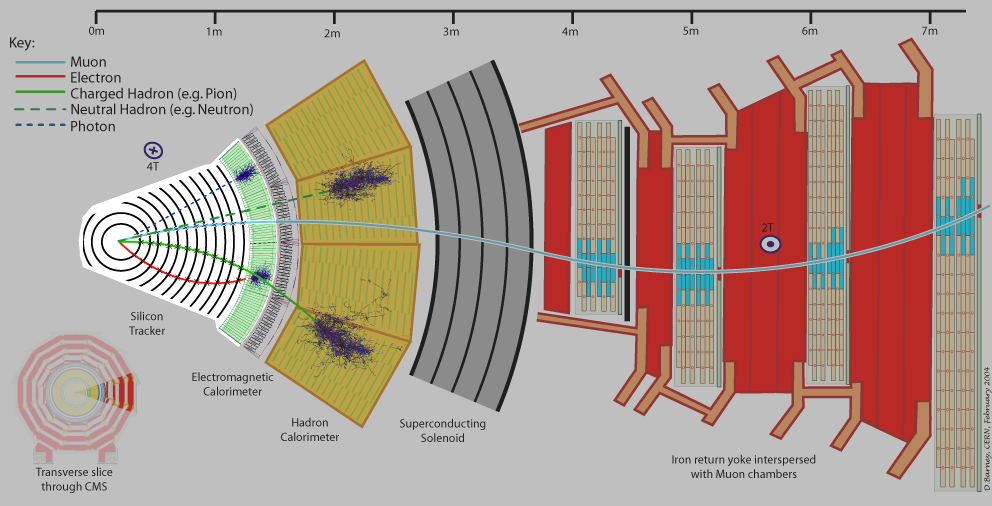
\includegraphics[width=0.75\textwidth]{figures/flowOfParticlesThroughCMS.png}
	\caption{Typical trajectories of particles travelling through CMS, from CERN.}
	\label{fig:particleTrajectories}
\end{figure}


\section{Track Reconstruction}
\label{sec:trkReco}
Muons and charged hadrons are reconstructed as helical tracks from signals measured in the silicon tracker.  An iterative algorithm 
starts by reconstructing tracks from signals in the inner pixel tracker, which are characterized by the highest energies or smallest 
distances from the IP.  The algorithm iterates to outer pixel and strip layers, and extends tracks by including new signals.  
Signals in successive layers are linked into continuous tracks using a Kalman filter that requires each signal to have 
$\chi^{2} <$ 30 \cite{trackerPerformanceInCollisions}.  Each time a new signal is added to a track, an analytic function 
extrapolates the track trajectory to the next layer assuming energy is lost only through ionization in the silicon.  Hits in 
the next layer are searched for in the region identified by the analytic extrapolation, and this procedure repeats 
until signals are included from the outermost silicon strip tracker layer.  Then, the signals linked into tracks are removed 
from the list of track candidates, and the algorithm restarts using signals measured in the inner pixel tracker characterized 
by lower energies or larger distances from the IP.  Using this algorithm, isolated muons with $\pt > 0.9$ $\GeV$ and $|\eta| < 2.4$ 
were reconstructed as tracks with essentially 100\% efficiency \cite{trackerPerformanceInCollisions}.  After reconstructing 
all tracks in an event, each point where two or more tracks originate is identified as an interaction vertex.  Each vertex is 
required to have at least two reconstructed track origins within 2 mm of the vertex position, and the vertex position is measured 
relative to the IP.  The positions of vertices that have muon tracks with $|\eta| < 1.4$ and $\pt = 100$ $\GeV$ 
were measured with 10 and 30 $\mu$m resolutions in the transverse (r-$\phi$) and longitudinal ($z$) directions.

Using a second track reconstruction algorithm, electrons are reconstructed as helical tracks from signals measured in the silicon 
tracker.  A second algorithm is used because the tracker contains 1 to 2 radiation lengths of material, which cause electrons to 
shower and lose energy through bremsstrahlung.  Due to the tracker material, $\sim$35\% of electrons that traverse the tracker lose 
more than 70\% of their initial energies through bremsstrahlung \cite{trackerPerformanceInCollisions}, and this energy cannot be 
measured by the tracker.  The electron track reconstruction algorithm uses the same iterative track reconstruction procedure described 
previously, but extrapolates each track's trajectory to the next silicon layer assuming the track loses energy through bremsstrahlung 
that is described by a sum of six Gaussians \cite{gsfFunction}.  The Gaussian widths can be any positive value, but their total width 
must minimize the difference in the cumulative probability function of the predicted energy loss between the Bethe-Heitler formula 
and the 6-Gaussian approximation.  Also, the Kalman filter used to link signals in successive layers requires that new signals 
have $\chi^{2} <$ 2000.  Using the electron track reconstruction algorithm, electrons that had $\pt > 20$ $\GeV$ and $|\eta| < 2.5$ 
were reconstructed as tracks with an efficiency $\geq$ 97\% \cite{gsfPerformanceInCollisions}.

\subsection{Muon Reconstruction}
\label{sec:muReco}
Muons are reconstructed as tracks from signals measured in individual muon chambers.  In each DT chamber\footnote{The 3 innermost radial 
layers of DTs use DT chambers that have 8 layers of r-$\phi$ measurement planes and 4 layers of r-z measurement planes.}, first the start 
and end points of track segments are identified as pairs of signals measured in the same plane (r-$\phi$ or r-z) but in different layers.  
Then, straight lines are drawn between the signal pairs, and a signal pair is ignored if its line does not point toward the IP.  The 
remaining signals that overlap with any of these straight lines are built into track segments 
that are measured in at least 3 layers.  In each plane the track segment that has signals in the largest number of layers ($N_{lay}$), at 
least 3, and the lowest $\chi^{2}/nDOF$ ($\chi^{2}_{min}$), less than 20, is used to build a 3D track.  If there are two or more track 
segments in one plane with the same $N_{lay}$ and $\chi^{2}_{min}$, then all combinations of r-$\phi$ and r-z track segments are 
used to build several 3D tracks.  In practice, more than one 3D track is reconstructed in a DT chamber in less than 1\% of events 
\cite{cmsTdrPhysPerformance}.  The same 
track segment reconstruction algorithm is used in each 6 layer, single plane CSC.  There, the final track segment must have signals 
in at least 4 layers.  In the barrel-endcap transition region ($1.3 < |\eta| < 1.6$) where the DT chambers stop and the CSCs begin, RPCs 
are used to improve the muon reconstruction efficiency and the precision of arrival time measurements.  Each RPC contains two parallel 
plates divided into many thin strips, and strips that measure a signal are grouped into clusters.  Each reconstructed cluster represents 
a hit whose position is the center of gravity of all the strips in the cluster.

Individual chamber tracks are connected to reconstruct muon trajectories over several meters.  
A Kalman filter algorithm starts with tracks in the chambers closest to the IP, and predicts the track positions in chambers in the next 
radial station with the effects of an inhomogeneous magnetic field and material losses taken into account \cite{muonRecoFirstCollisions}.  
Track segments in outer chambers are added to existing tracks subject to a $\chi^{2}$ requirement, and existing tracks are propagated to 
the next radial station even if no matching track segment is found in the current station.  Once the outermost station is included, a 
reverse Kalman filter is applied to reconstructed tracks from the outermost to the innermost station.  The reverse Kalman filter finalizes 
the track parameters, then these tracks are compared to silicon tracker tracks to identify muons.

Muons are identified using tracks reconstructed in the silicon tracker and muon detectors.  Tracks from the muon detectors are 
extrapolated to the outermost silicon strip tracker layer, where their $(\eta,\phi)$ positions are compared to those of silicon tracker 
tracks.  In the local coordinate plane of the silicon strip layer, each silicon tracker track that passes within 3 cm of a muon detector 
track is identified as a muon.  If an extrapolated muon detector track has multiple silicon tracker track candidates within 3 cm, the 
closest match is identified as a muon.  The silicon tracker track determines the $(\eta,\phi)$ trajectory of each muon.

The momentum of each muon is determined by sampling four different muon reconstruction algorithms, and selecting the  
highest quality result.  Each algorithm fits a continuous track \cite{cmsMuonRecoRunTwo} to a unique combination of silicon tracker 
and muon detector signals to estimate a muon's trajectory through CMS, depicted in Figure \ref{fig:particleTrajectories}.  The 
quality of each continuous track is identified by a fit uncertainty $\chi^{2}/nDOF$ and momentum uncertainty $\sigma(\pt)/\pt$.  The 
track with the lowest $\chi^{2}/nDOF$ and momentum uncertainty $\sigma(\pt)/\pt < 0.3$ determines the muon's momentum.  
For muons with $\pt \lesssim 100$ $\GeV$ the highest quality result is obtained using only silicon tracker measurements.  Muons that had 
$|\eta| < 1.4$ and $\pt = 100$ $\GeV$ were measured with a $\pt$ resolution of $\sim$2.8\% \cite{trackerPerformanceInCollisions}.  
As a muon's $\pt$ increases above 100 $\GeV$ the silicon tracker $\pt$ resolution degrades faster that that of the muon 
detectors.  A significant fraction of $\WR \rightarrow \mu\mu jj$ events are expected to produce at least one muon with $\pt > 200$ $\GeV$ 
(Table \ref{tab:wrHighPtMuons}), and in this high $\pt$ region the highest quality momentum measurement comes from combining silicon 
tracker and muon detector measurements.  By combining measurements, muons with $|\eta| < 0.9$ and $200 < \pt < 400$ $\GeV$ were measured 
with a $\pt$ resolution of 3.2\%; higher $\pt$ muons were measured with a resolution better than 6\% \cite{cmsMuonRecoRunTwo}.

\begin{table}[h]
	\caption{Fraction of expected $\WR \rightarrow \mu\mu jj$ events that had at least one muon with $\pt > 200$ $\GeV$. 
	($\mnul = \frac{1}{2}\mWR$)}
	\label{tab:wrHighPtMuons}
	\centering
	\begin{tabular}{c|c}
		\mWR ($\TeV$) & Fraction of events with at least one high-$\pt$ muon (\%) \\  \hline
		1.0 &  80.  \\
		2.0 &  95.  \\ 
		3.0 &  98.  \\ \hline
	\end{tabular}
\end{table}

Muons reconstructed in simulated events have slightly different energies than muons reconstructed in data.  Energy corrections for simulated 
muons are derived using $Z \rightarrow \mu\mu$ events from simulations and data.  The di-muon mass ($M_{\mu\mu}$) distribution in 
$Z \rightarrow \mu\mu$ events is compared between data and simulations, and the energies of simulated muons are corrected so that the two 
$M_{\mu\mu}$ distributions match.  The average correction is 1\% of a muon's $\pt$.


\section{Energy Measurement}
\label{sec:enrgReco}
The energies of photons and electrons produced in pp interactions are measured in groups of ECAL crystals.  Photons and electrons 
impinging on the ECAL generate signals in the ECAL crystals that are converted into uncalibrated energies.  The most energetic crystals 
with $\Et \gtrsim 0.2$ $\GeV$ and their nearest neighbors are grouped into superclusters (SCs) that are at least 3 crystals wide in 
$\eta$.  The upstream tracker material causes $\sim$35\% of electrons and photons to shower early in the tracker 
\cite{trackerPerformanceInCollisions}, and the magnetic field spreads the shower over several crystals in $\phi$.  To capture the early 
shower energy, each SC is at least 5 crystals wide in $\phi$, and can be much larger, as in Figure \ref{fig:eleTrackAndSC}.  Once a SC 
is built, the energy of each crystal in the SC is multiplied by a laser transparency correction, and relative and absolute energy 
calibration corrections.  The sum of the calibrated crystal energies is the SC energy, and the energy weighted average $(\eta,\phi)$ 
position is the SC position.  Using only ECAL SCs, the $(\eta,\phi)$ positions of electrons in the barrel (endcap) were measured with 
a $\phi$ resolution of 0.17$^{\circ}$ (0.29$^{\circ}$), and an $\eta$ resolution of 0.001 (0.002) units.

The energies of hadrons are measured over 10 nuclear interaction lengths of material, the first of which is the lead tungstate ECAL.  
Up to 25\% of hadrons start showering in the tracker \cite{trackerPerformanceInCollisions}, so hadrons impinging on the ECAL are 
reconstructed as SCs like electrons and photons.  Hadrons impinging on the HCAL generate 
signals in the HCAL towers that are converted into uncalibrated energies.  The highest energy towers with $\Et \gtrsim 1$ $\GeV$ are 
used to seed tower clusters, which include all neighboring towers that have $\Et > 0.8$ $\GeV$ \cite{pflowEventReco}.  If one tower is 
grouped into multiple clusters, the tower's contribution to each cluster is weighted by its distance from each cluster's seed.  After 
the clusters are built, each tower's energy is multiplied by a laser transparency correction, and relative and absolute energy calibration 
corrections.  The sum of the calibrated tower energies is the cluster energy, and the energy weighted average $(\eta,\phi)$ position is 
the cluster position.  Combining ECAL and HCAL energy measurements, hadrons that have $\Et = 100$ $\GeV$ were measured with a $\sim$10\% 
$\Et$ resolution \cite{pflowEventReco}.

\subsection{Electron, Photon, and Hadron Reconstruction}
\label{sec:elePhoHadReco}
A track is identified as being caused by an electron using ECAL SCs.  Reconstructed tracks are extrapolated from the outermost silicon strip 
layer to the front face of the ECAL, where their $(\eta,\phi)$ positions are compared to those of ECAL SCs.  If one or more tracks match a SC's 
$(\eta,\phi)$ position within 1.0$^{\circ}$ (1 crystal wide) in $\phi$, and within 0.004 units (below $\frac{1}{2}$ a crystal wide) in $\eta$, then 
the track and ECAL SC are identified as an electron candidate.  If the ECAL SC $\Et$ and the matched track $\pt$(s) agree within the track 
$\pt$ uncertainty, then the track and SC are identified as an electron.  Using the SC energy, electrons with $\Et \approx 45$ $\GeV$ and 
$|\eta| < 0.8$ were measured with an $\Et$ resolution better than 2\%, and a resolution between 2\% and 5\% at higher $|\eta|$ 
\cite{ecalPerformanceInCollisions}.

\begin{figure}[h]
	\centering
	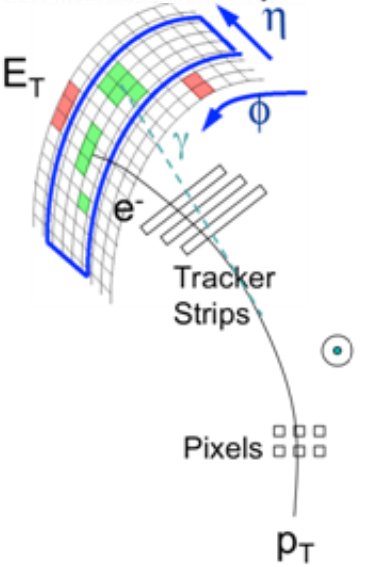
\includegraphics[width=0.3\textwidth]{figures/electronTrackAndSupercluster.png}
	\caption{The trajectory of a typical electron through the tracker and the ECAL.}
	\label{fig:eleTrackAndSC}
\end{figure}

Electrons reconstructed in simulated events have slightly different energies than electrons reconstructed in data.  Energy corrections for 
simulated electrons are derived using $Z \rightarrow ee$ events from simulations and data.  The di-electron mass ($M_{ee}$) 
distribution in $Z \rightarrow ee$ events is compared between data and simulations, and the energies of simulated electrons 
are corrected so that the two $M_{ee}$ distributions match.  The average correction is 1\% of an electron's $\Et$.

After electrons are identified, ECAL SCs are identified as being caused by photons using the remaining reconstructed tracks.  An ECAL SC that does 
not match any reconstructed track within the electron track-SC $(\eta,\phi)$ window is identified as a photon.  Alternatively, an ECAL SC that 
matches a reconstructed track within the electron track-SC $(\eta,\phi)$ window is identified as a photon if its $\Et$ does not agree with the track 
$\pt$ within the track $\pt$ uncertainty.

A reconstructed track is identified as being caused by a charged hadron using the calorimeter energy clusters.  A track that is not 
identified as an electron is extrapolated from the outermost silicon strip layer to the HCAL front face, and its $(\eta,\phi)$ position is 
compared to that of the HCAL clusters.  If a track intersects with any portion of an HCAL cluster, and the cluster $\Et$ and track $\pt$ agree 
within the cluster $\Et$ uncertainty, then the track is identified as a charged hadron.  The track $\pt$ and $(\eta,\phi)$ characterize the charged 
hadron kinematics.
%If an ECAL SC that is not associated with an electron overlaps with any portion of the HCAL cluster, then the ECAL SC can 
%be incorporated into the charged hadron.  The ECAL SC is incorporated into the charged hadron if the ECAL $\plus$ HCAL $\Et$ is 
%consistent within its uncertainty with the matching track $\pt$.

After all charged tracks are identified as leptons or hadrons, an HCAL cluster that is not intersected by a track is identified as a 
neutral hadron.  Also, an HCAL cluster that is intersected by a track is identified as a neutral hadron if its $\Et$ does not agree with 
the track $\pt$ within the $\Et$ uncertainty.  If an ECAL SC (energy $E_{ECAL}$, uncertainty $\delta E_{ECAL}$) 
overlaps with any portion of an HCAL cluster (energy $E_{HCAL}$, uncertainty $\delta E_{HCAL}$) identified as a neutral hadron, then the 
SC can be identified as a neutral hadron.  The ECAL SC is identified as a neutral hadron if $E_{ECAL}$ and $E_{HCAL}$ agree within the larger 
of the two uncertainties $\delta E_{ECAL}$ and $\delta E_{HCAL}$.  The $\Et$ and $(\eta,\phi)$ trajectory of each neutral hadron is determined 
by the calorimeter $\Et$s, and the $\Et$-weighted average cluster position relative to the IP.


\subsection{Jet Reconstruction}
\label{sec:jetReco}
Quarks and gluons emitted from pp interactions produced jets of photons, hadrons and leptons.  On average, 85\% of a jet's 
energy is carried by charged particles and photons \cite{pflowJetRecoInCollisions}, so during jet reconstruction these particles are 
reconstructed first.  The particle flow jet reconstruction algorithm \cite{pflowEventReco} identifies $(\eta,\phi)$ regions with one or 
more silicon tracker or muon detector tracks, one or more HCAL clusters, and any number of ECAL SCs.  In these regions, algorithms 
described previously are used to reconstruct muons first, followed by electrons and photons and charged hadrons, then neutral hadrons.  
After all tracks and energy clusters in a region are identified as specific particles, a jet, represented by the cone in Figure 
\ref{fig:jetClustering}, is clustered from those particles.

Due to the high instantaneous collision luminosity, each pp bunch crossing delivered by the LHC produces multiple pp interactions, 
or pileup (PU) interactions, that make jet clustering more challenging.  In every unit of $\eta$, each PU interaction adds 
$\sim$11 charged particle tracks with $\pt \approx 0.5$ $\GeV$ to the event \cite{chgdHdrMultInData}.  These tracks are primarily 
charged hadrons, so before jets are clustered the charged hadrons associated with PU interaction vertices are removed from 
all jet clustering regions.  Jets are then clustered from reconstructed particles using the anti-$k_{T}$ algorithm \cite{antikt} 
with a distance parameter $R = 0.4$.  In each region the anti-$k_{T}$ algorithm starts with the highest $\pt$ hadron and adds 
other particles to the jet based on their $\pt$ and distance from the jet axis.  Using the distance parameter $R = 0.4$, 
particles located $\Delta R > 0.4$ from the jet axis are less likely to be clustered into the jet than particles located within 
$\Delta R \leq 0.4$.  Once anti-$k_{T}$ jets are clustered a second set of smaller jets are clustered to estimate the average 
increase in jet energy due to neutral particles produced in PU interactions.  The second set of jets are clustered from 
reconstructed particles using the $k_{T}$ algorithm \cite{ktAlgoOne,ktAlgoTwo,ktAlgoThree} with distance parameter $R = 0.3$.  
Then each $k_{T}$ jet's $\pt$ is divided by its area ($\pt_{j} / A_{j}$), and the median value $\rho$ is the average neutral 
particle energy density in the event \cite{pileup1,pileup2}.  Each PU interaction increases $\rho$ by about 0.5 $\GeV$ 
\cite{jetResolutionInCollisions}.  Using the hybrid jet area subtraction technique described in \cite{pflowJetRecoInCollisions}, 
the photon and neutral hadron energies in each anti-$k_{T}$ jet are reduced by multiplying $\rho$ by the jet's area and and $\eta$ 
dependent factor.  After the area based subtraction, jet energies are calibrated to correct for known $\eta$ and $\pt$ variations 
of the detector's response to jets.  After calibrations, particle flow jets with $\pt > 40$ $\GeV$ and $|\eta| < 1.3$ were 
measured with a $\pt$ resolution of 16\% or better \cite{jetResolutionInCollisions}.

\begin{figure}[h]
	\centering
	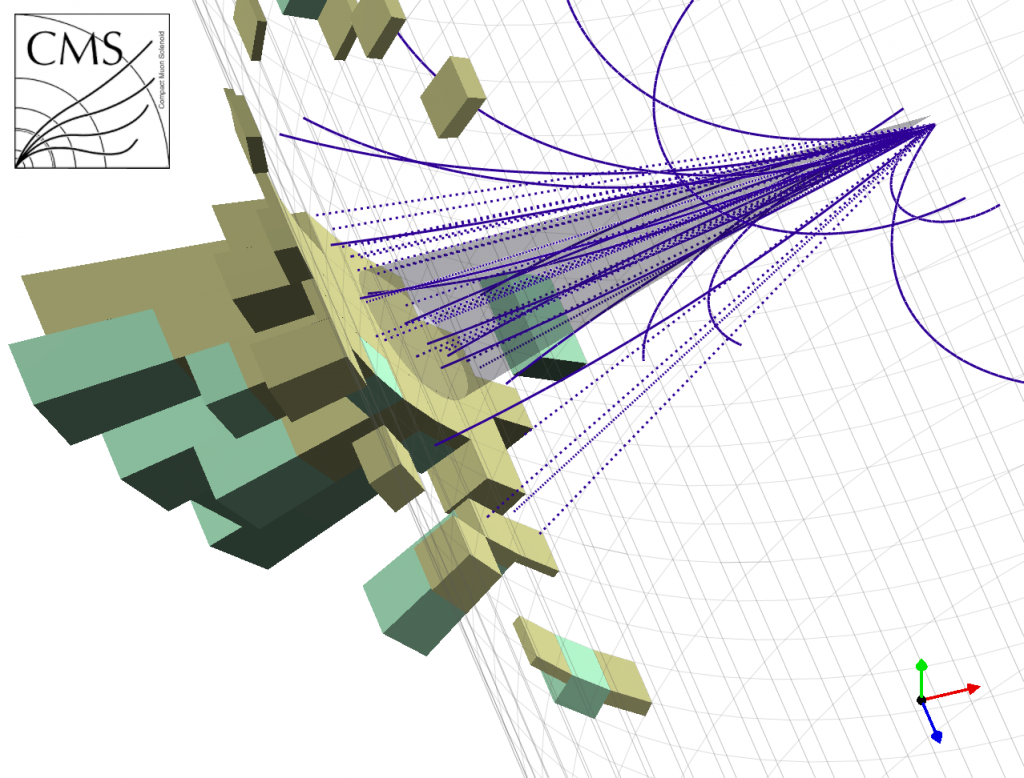
\includegraphics[width=0.45\textwidth]{figures/jetClusteringInCMS.png}
	\caption{A cone of reconstructed particles clustered into a jet, with the reconstructed vertex on the right.  
	From the CMS Experiment.}
	\label{fig:jetClustering}
\end{figure}

Jets reconstructed in simulated events have slightly different energies than jets reconstructed in data.  Energy corrections for 
simulated jets are derived using dijet, $Z$+jet, and $\gamma$+jet events found in simulations and data \cite{jetpaper}.  The di-jet 
mass and leading jet $\pt$ distributions found in these events are compared between data and simulations, and the energies of simulated 
jets are corrected so that the jet distributions match.  The average correction is 6\% of a jet's $\pt$.


\section{Trigger and Offline Selection Criteria}
\label{sec:onlineAndOfflineIdSel}
During collisions, the electron, muon, and HCAL cluster reconstruction algorithms are used in electron and muon triggers to select 
events with at least one lepton that is isolated from large HCAL energies.  The triggers used for the $\mu\mu$-channel and the $ee$-channel 
were chosen to maximize the \WR selection efficiency, and select a large fraction of $Z \rightarrow \ell\ell$ events to minimize the 
statistical uncertainty on the \DY background prediction discussed later.

Single muon and double-muon triggers select $\WR \rightarrow \mu\mu jj$ events with different efficiencies.  The single muon 
triggers require one track segment to be reconstructed in multiple muon detectors and have $\pt$ above some threshold $A$, while the 
double-muon triggers require two track segments that have $\pt$ above some threshold $B < A$.  In simulated $\WR \rightarrow \mu\mu jj$ 
events the highest efficiency single muon trigger selected 5\% more \WR events than the highest efficiency double muon trigger (Table 
\ref{tab:singleVsDblMuHlt}).  The double-muon trigger selected fewer \WR events because the efficiency to reconstruct a muon with 
$\pt > B$ as a track segment was below 100\% \cite{cmsMuonRecoRunTwo}.  To maximize the signal selection efficiency, a single muon 
trigger was used to select collision events with muons.

\begin{table}[h]
	\caption{The efficiency of a single and double-muon trigger in simulated $\WR \rightarrow \mu\mu jj$ events with $\mWR = 800$ $\GeV$ 
		and $\mnul = 400$ $\GeV$.}
	\label{tab:singleVsDblMuHlt}
	\centering
	\begin{tabular}{c|c|c}
		trigger type & $\pt$ criteria & efficiency (\%) \\  \hline
		single $\mu$ & $\pt >50$ $\GeV$ & 98  \\ 
		double-$\mu$ & one $\pt >17$, other $\pt >8$ $\GeV$ & 93  \\
	\end{tabular}
\end{table}

During collisions, events with muons were selected using a Level-1 trigger that required one track segment with $\pt > 16$ $\GeV$.  The 
segment was required to have signals in DT or CSC chambers from at least 2 stations, and signals in at least 4 layers of each chamber.  
Then, events were required to pass the following single muon HLT selection criteria:

\begin{itemize}
	\item A track was reconstructed in the silicon tracker with $\pt > 50$ $\GeV$ and $|\eta| < 2.4$.
	\item In the plane perpendicular to the beam axis, the distance between the silicon tracker track origin and its 
		reconstructed vertex was $< 1$ mm.
	\item The muon detector track that passed the L1 trigger extrapolated back to the silicon tracker track $(\eta,\phi)$ 
		position to within 3 cm.
\end{itemize}

Muons reconstructed in simulated events passed the trigger criteria with a different efficiency than muons reconstructed in data.  This 
efficiency difference was corrected by multiplying the weight of every simulated event (default weight is 1.0) by a $\pt$,$\eta$-
dependent value between 0.95 (5\% decrease) and 1.04 (4\% increase) for the muon that fired the trigger.

In events selected by the single muon trigger, tracks in the muon detectors and silicon tracker were identified as being caused by muons 
using algorithms described previously.  Then, the following identification criteria were applied to select promptly produced muons 
that were isolated from other particles and reconstructed in multiple muon stations:

\begin{itemize}
	\item The muon track reconstructed in the silicon tracker:
	\begin{itemize}
		\item Was reconstructed from signals in at least 1 silicon pixel detector layer, and signals in at least 
			5 layers in the entire tracker.
		\item Within a cone of radius $\Delta R = 0.3$ centered on the track, the $\sum \pt$ of all other 
			reconstructed tracks was low compared to the muon $\pt$, $\frac{\sum \pt}{muon \pt} < 0.1$.
	\end{itemize}
	\item The muon's track segment went through a muon chamber in at least 2 muon stations.  Track segments in each DT 
		chamber were required to have signals in all 4 r-$z$ layers, and at least 7 of 8 r-$\phi$ layers.  Track segments 
		in each CSC were required to have signals in all 6 layers.
	\item The origin of the muon's silicon tracker track was within 2 mm of the muon's reconstructed vertex 
		position along the $z$ axis.
\end{itemize}

Simulated muons are reconstructed and pass the offline muon identification selection criteria with a higher 
efficiency than muons produced in real collisions.  This efficiency difference was corrected by multiplying the weight of every 
simulated event by a $\pt$,$\eta$-dependent value between 0.985 and 1.0 for each offline muon selected in the event.


Similar to the muon triggers, single electron and double-electron triggers select $\WR \rightarrow eejj$ events with different efficiencies.  
The single electron triggers require that one track reconstructed in the silicon tracker extrapolates to a 5 $\times$ 5 ECAL crystal 
cluster with $\Et$ above some threshold $D$, while the double-electron triggers require two such track-ECAL cluster combinations each 
with $\Et$ above some threshold $G < D$.  In simulated $\WR \rightarrow eejj$ events the highest efficiency single and double-electron 
triggers selected similar numbers of signal events (Table \ref{tab:singleVsDblEleHlt}), so a trigger was chosen using different criteria.  To 
reduce the statistical uncertainty on the \DY background prediction, the electron trigger should select a large fraction of $Z \rightarrow ee$ 
events.  The single electron trigger required $\Et > 105$ $\GeV$, thereby excluding a significant fraction of $Z \rightarrow ee$ events.  To 
select a larger portion of $Z \rightarrow ee$ events, a double-electron trigger that required two electrons that had $\Et > 33$ $\GeV$ 
was used to select collision events with electrons.

\begin{table}[h]
	\caption{The efficiency of a single and double-electron trigger in simulated $\WR \rightarrow \mu\mu jj$ events with $\mWR = 800$ $\GeV$ 
		and $\mnul = 400$ $\GeV$.}
	\label{tab:singleVsDblEleHlt}
	\centering
	\begin{tabular}{c|c|c}
		trigger type & $\Et$ criteria & efficiency (\%) \\  \hline
		single $e$ & $\Et >105$ $\GeV$ & 94  \\ 
		double-$e$ & both $\Et >33$ $\GeV$ & 92  \\
	\end{tabular}
\end{table}

During collisions, events with electrons were selected using single and double-electron Level-1 triggers.  These triggers required 
one 5 $\times$ 5 ECAL crystal cluster that had $\Et > 40$ $\GeV$, or two 5 $\times$ 5 ECAL clusters that had 
$\Et > 22$ $\GeV$ and $\Et > 10$ $\GeV$.  Then, events were required to pass the following double-electron HLT selection criteria:

\begin{itemize}
	\item Two 5 $\times$ 5 ECAL crystal clusters separated by $\Delta R > 0.1$ were required to have $\Et > 33$ $\GeV$.
	\item For each ECAL cluster (energy E):
	\begin{itemize}
		\item The hadronic energy behind the cluster was $<$ 15\% of E in the barrel, and $<$ 10\% of E in the endcap. 
		\item Ninety percent of E was measured in an area that was two crystals wide in $\eta$.
		\item If the cluster was in the barrel, a reconstructed track with signals in at least two pixel tracker layers 
			extrapolated close to the cluster position.  The track extrapolated from the pixel tracker to within $2.3$ cm 
			of the cluster $z$ position, and to within 1 ECAL crystal area of the cluster $(\eta,\phi)$ position.
	\end{itemize}
\end{itemize}

Electrons reconstructed in simulations passed the trigger criteria with the same efficiency as electrons that were reconstructed in data, 
so no electron trigger efficiency correction was applied to simulated events.

In events selected by the double-electron trigger, reconstructed tracks and ECAL SCs were identified as being caused by electrons using 
algorithms described previously.  Then, the following identification criteria were applied to select the promptly produced electrons, 
excluding electrons within a jet, or in the ECAL transition region $1.44 < |\eta| < 1.57$:

\begin{itemize}
	\item The electron $\Et$ is the calibrated ECAL SC energy $E_{SC}$.
	\item For a SC in the barrel, at least 94\% of $E_{SC}$ was measured in an area that was 2 crystals wide in $\eta$.
	\item The hadronic energy (H) behind the SC was $\frac{H}{E_{SC}}< 0.05 +\thickspace \frac{1 \GeV}{E_{SC}}$ 
		in the barrel, and $\frac{H}{E_{SC}}< 0.05 +\thickspace \frac{5 \GeV}{E_{SC}}$ in the endcap.
	\item In a $\Delta R =$ 0.3 radius cone centered on the electron's $(\eta, \phi)$ trajectory:
	\begin{itemize}
		\item The $\sum \pt$ of all tracks excluding the electron's track was low, $\sum \pt < 5$ $\GeV$.
		\item The total calorimeter energy $E_{ECAL + HCAL}$ not associated with the electron was 
			$E_{ECAL + HCAL} < 2 + 0.03\alpha + 0.28\rho$.  $\rho$ is the neutral particle energy per unit $\eta,\phi$ area, 
			$\alpha$ in the barrel is $E_{SC}$, and $\alpha$ in the endcap is $E_{SC} - 50$.
	\end{itemize}
	\item For a SC in the endcap, the electron track extrapolated from the outermost silicon tracker measurement to the SC 
		seed crystal position to within $\sim$3 crystal widths in $\phi$.
	\item The electron track was reconstructed from signals in every silicon pixel and inner strip detector layers, or all but 1 layer.
	\item The electron track's origin was separated from its vertex by a small distance $\Delta_{xy}$ in the $x-y$ 
		plane: $\Delta_{xy} < 0.2$ mm in the tracker barrel, and $\Delta_{xy} < 0.5$ mm in the tracker endcap.
\end{itemize}

Simulated electrons are reconstructed and pass the offline electron identification selection criteria with a higher efficiency than 
electrons that were reconstructed in data.  This efficiency difference was corrected by multiplying the weight of every 
simulated event by 0.982, the reconstruction efficiency correction, and by 0.989, the ID efficiency correction, for each offline electron 
selected in the event.

In events selected by the lepton triggers, jets were reconstructed offline from tracks and calorimeter energy clusters using the 
algorithms described previously.  Then, the following identification criteria were applied to select jets that contained at least one 
charged hadron, and whose energies were not dominated by electron or photon SCs:

\begin{itemize}
	\item The jet had at least 2 constituents.
	\item The jet had at least 1 charged hadron constituent.
	\item More than 0\% of the total jet energy came from charged hadrons.
	\item Less than 90\% of the total jet energy came from neutral hadrons.
	\item Less than 90\% of the total jet energy came from photons.
	\item Less than 99\% of the total jet energy came from electrons.
\end{itemize}

The efficiency with which jets are reconstructed and selected using the jet ID criteria is identical in data and simulations, so 
no jet efficiency corrections were applied in simulations.


\section{\WR Kinematics and Offline Kinematic Selection Criteria}
\label{sec:signalAndBkgnds}
The offline identification selection criteria were used to select events where an interaction produced two real leptons and jets, 
and their signals in the detector were correctly reconstructed as two leptons and jets.  These selection criteria were used in other 
searches for heavy particles that decay to leptons and jets \cite{exoLeptJetResults}, and were not optimized based on the kinematics of 
the \WR progeny.

The heavy \WR decays through a lighter \nul to two leptons and two jets according to the following decay chain:

\begin{equation}
	\WR \rightarrow \nul \plus \ell ; \quad \nul \rightarrow \ell jj
\end{equation}
%\begin{tikzpicture}[grow=right]
%	\node (Wr) at (0,0) {$\WR \thickspace \rightarrow \thickspace \nul + \ell$};
%	\node (Ar) at (0.75,-0.4) {$\searrow$};
%	\node (Nl) at (1.25,-0.75) {$\ell jj$};
%\end{tikzpicture} $\newline$
Since the \WR and \nul are assumed to couple to leptons and quarks with the same strengths as the $W$, the \WR and \nul lifetimes are 
shorter than the $W$ lifetime.  Therefore, the \WR and \nul decay promptly to leptons, and quarks that hadronize into jets.

The kinematics of leptons and jets produced in \WR decays are governed by \mWR and the ratio $\mnul/\mWR$.  Since \mWR is expected to be 
several $\TeV$ the \WR has low net momentum, so in the lab frame the \WR progeny \nul and $\ell$ are emitted isotropically.  In addition, 
the leptons and jets have high $\pt$ (Figure \ref{fig:wrLeptJetPts}), and are emitted at low $|\eta|$ 
(Figure \ref{fig:wrLeptJetEtas}).  At a specific \mWR, the ratio $\mnul/\mWR$ affects how the total energy \mWR is split amongst the leptons 
and jets, and their $(\eta,\phi)$ trajectories.  As $\mnul/\mWR$ approaches 1 the average energy of the $\ell_{1}$, from 
$\WR \rightarrow \ell_{1}\nul$, decreases, and the average \nul energy increases.  In general as $\mnul/\mWR$ increases, the transverse 
energies of the jets and one lepton increase, at the cost of the other lepton's energy (Figure \ref{fig:wrLeptQrkPtsVarMNu}).  For $\mnul \sim \mWR$ 
the decay $\nul \rightarrow \ell_{2}jj$ exemplifies the decay of a slow moving heavy particle into lighter particles: in the lab 
frame the $\ell_{2}$ and both jets are emitted isotropically.  Conversely, as $\mnul/\mWR$ approaches 0 the average $\ell_{1}$ energy 
increases, the average \nul energy decreases, but the average \nul momentum increases (Figure \ref{fig:hvyNuMomentumVarMNu}).  Here the decay 
$\nul \rightarrow \ell_{2}jj$ exemplifies the decay of a fast moving particle: in the lab frame the \nul progeny are boosted in the 
\nul momentum direction, and the $\Delta R(\ell,j)$ separation decreases (Figure \ref{fig:wrDrLeptQrkVarMNu}).  The \nul and $\ell_{1}$ 
recoil against each other, and the boost at low $\mnul/\mWR$ increases the angle between $\ell_{1}$ and $\ell_{2}$ (Figure 
\ref{fig:wrLeptAngleSepVarMNu}).  As a result, the di-lepton invariant mass ($\Mll$), proportional to the angle between the leptons, 
increases as $\mnul/\mWR$ approaches 0 (Figure \ref{fig:wrMllVarMNu}).

%to draw a plot of the angle between the two leptons use this argument in TTree Draw within quotes, and multiplied by 180/3.1416
% TMath::ACos(1-( (TMath::CosH(etaEle[0]-etaEle[1]) - TMath::Cos(phiEle[0]-phiEle[1]))/(TMath::CosH(etaEle[0])*TMath::CosH(etaEle[1]))  ))

\clearpage

\begin{figure}
	\centering
	\begin{subfigure}[t]{2.4in}
		\centering
		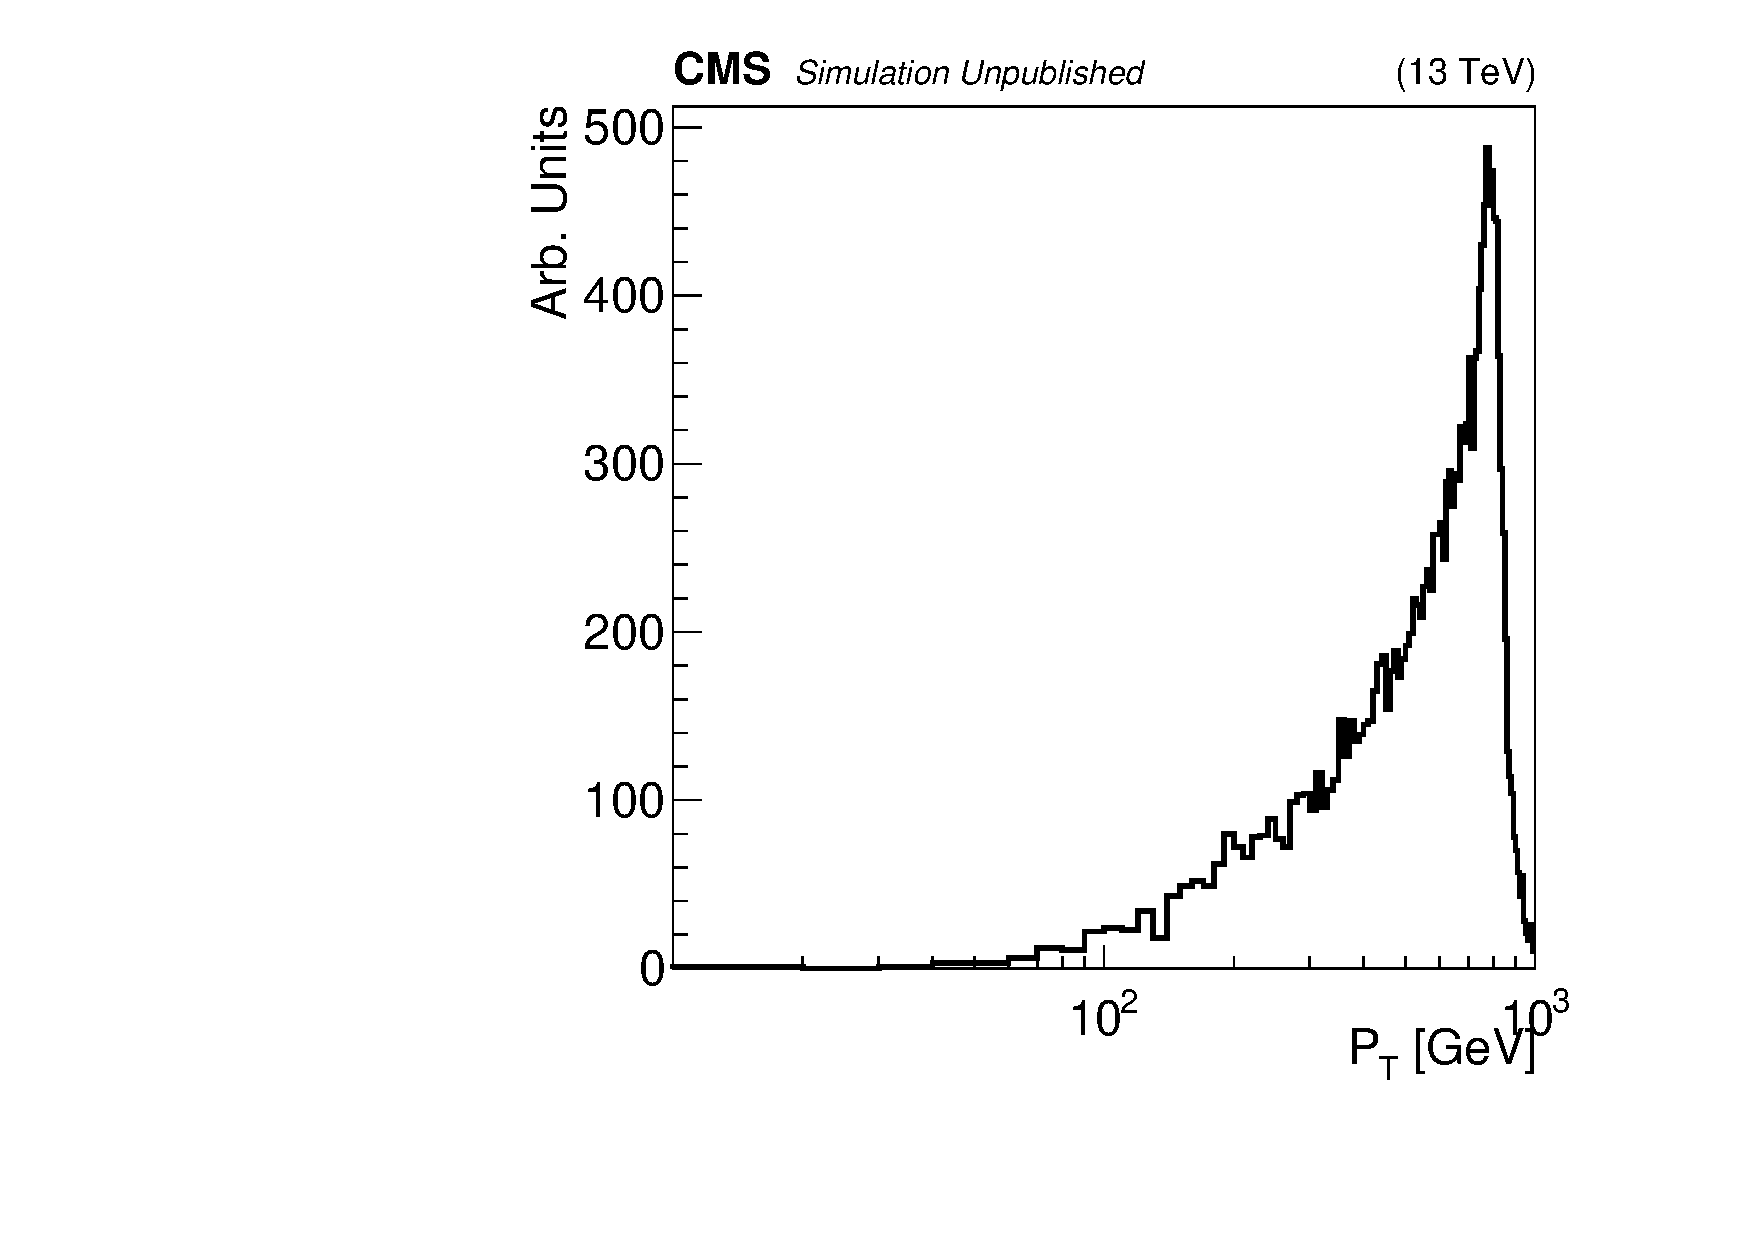
\includegraphics[width=2.4in]{figures/ptMatchedRecoEleFromWr_mwr2200_mnu1100.pdf}
		\caption{$\ell$ from $\WR \rightarrow \ell\nul$}\label{fig:wrLeptJetPtsa}
	\end{subfigure}
	\thickspace
	\begin{subfigure}[t]{2.4in}
		\centering
		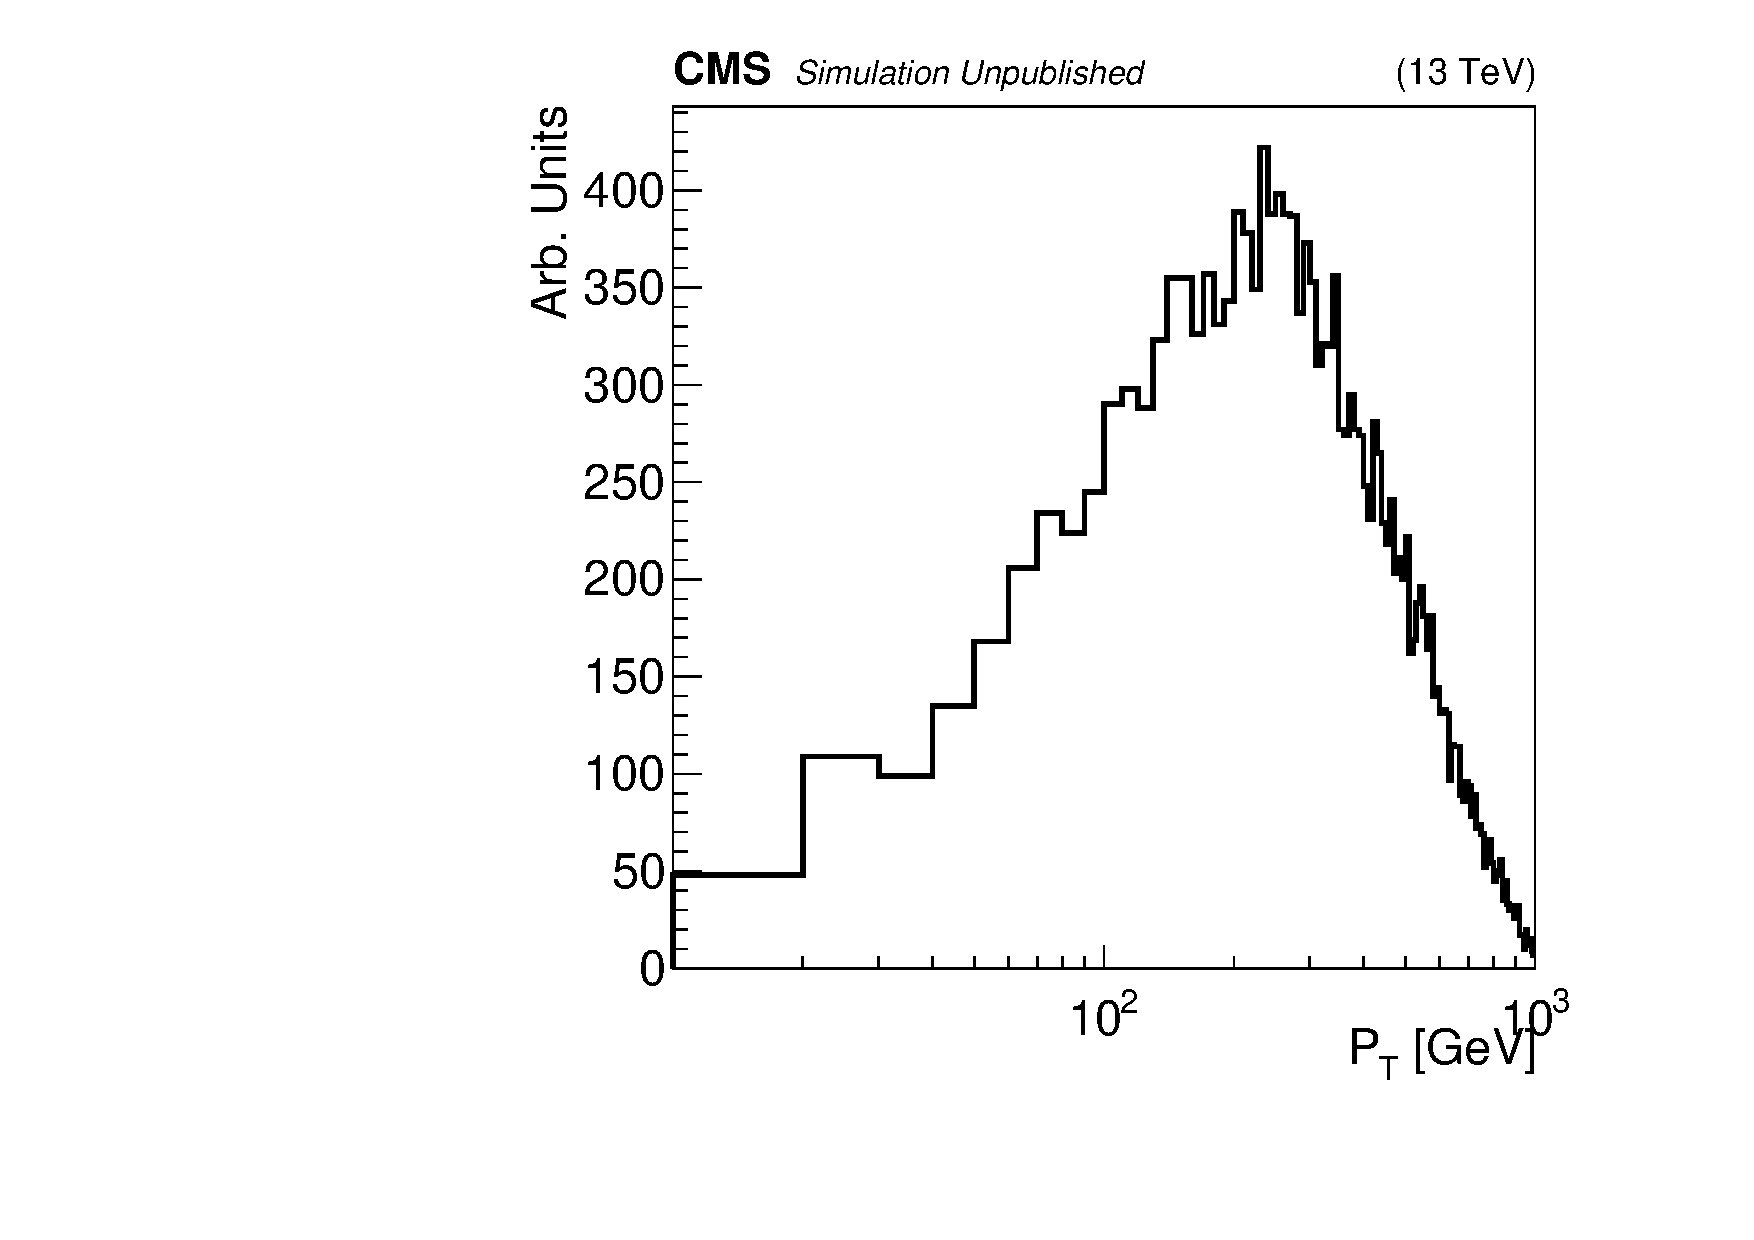
\includegraphics[width=2.4in]{figures/ptMatchedRecoEleFromNu_mwr2200_mnu1100.pdf}
		\caption{$\ell$ from $\nul \rightarrow \ell jj$}\label{fig:wrLeptJetPtsb}
	\end{subfigure}
	\newline
	\newline
	\newline
	\newline
	\begin{subfigure}[t]{2.4in}
		\centering
		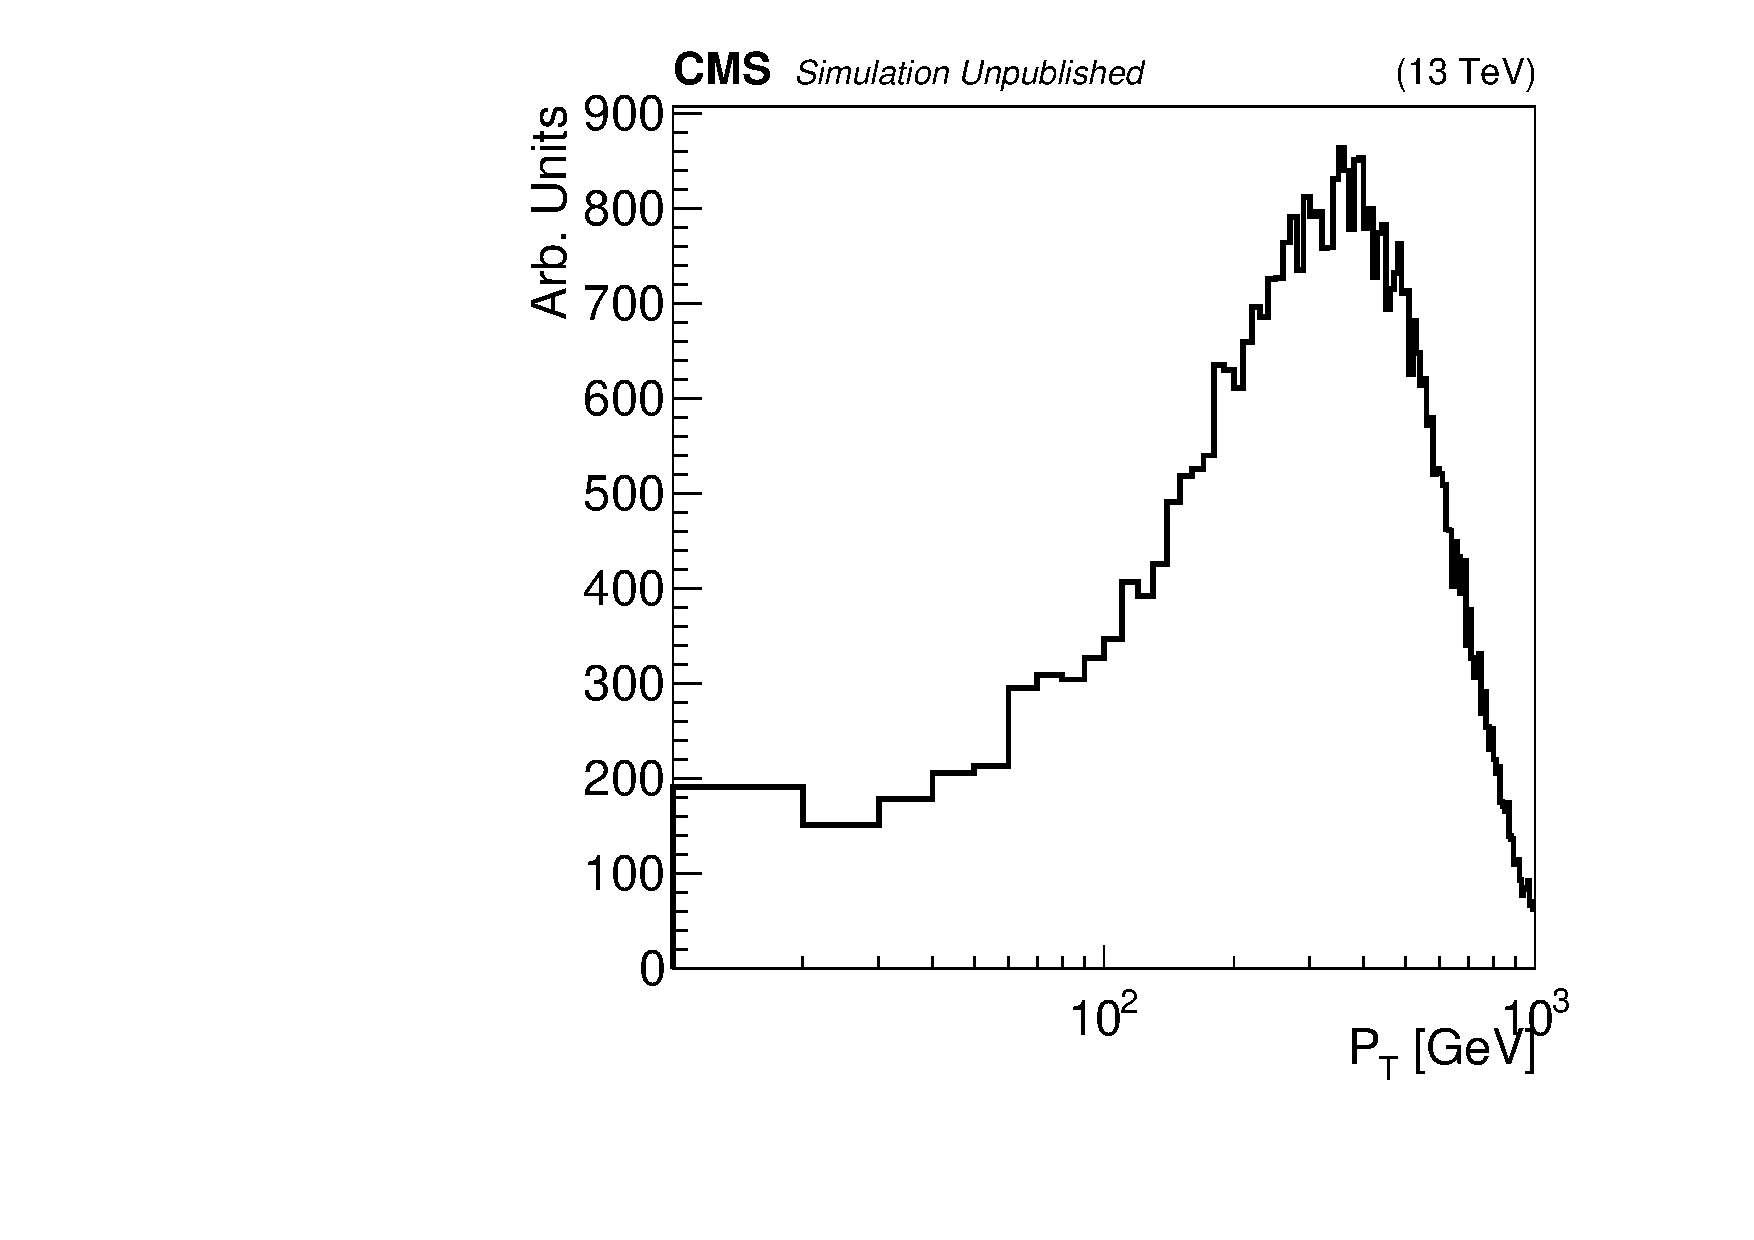
\includegraphics[width=2.4in]{figures/ptMatchedRecoJetOne_mwr2200_mnu1100.pdf}
		\caption{jet from $\nul \rightarrow \ell jj$}\label{fig:wrLeptJetPtsc}
	\end{subfigure}
	\thickspace
	\begin{subfigure}[t]{2.4in}
		\centering
		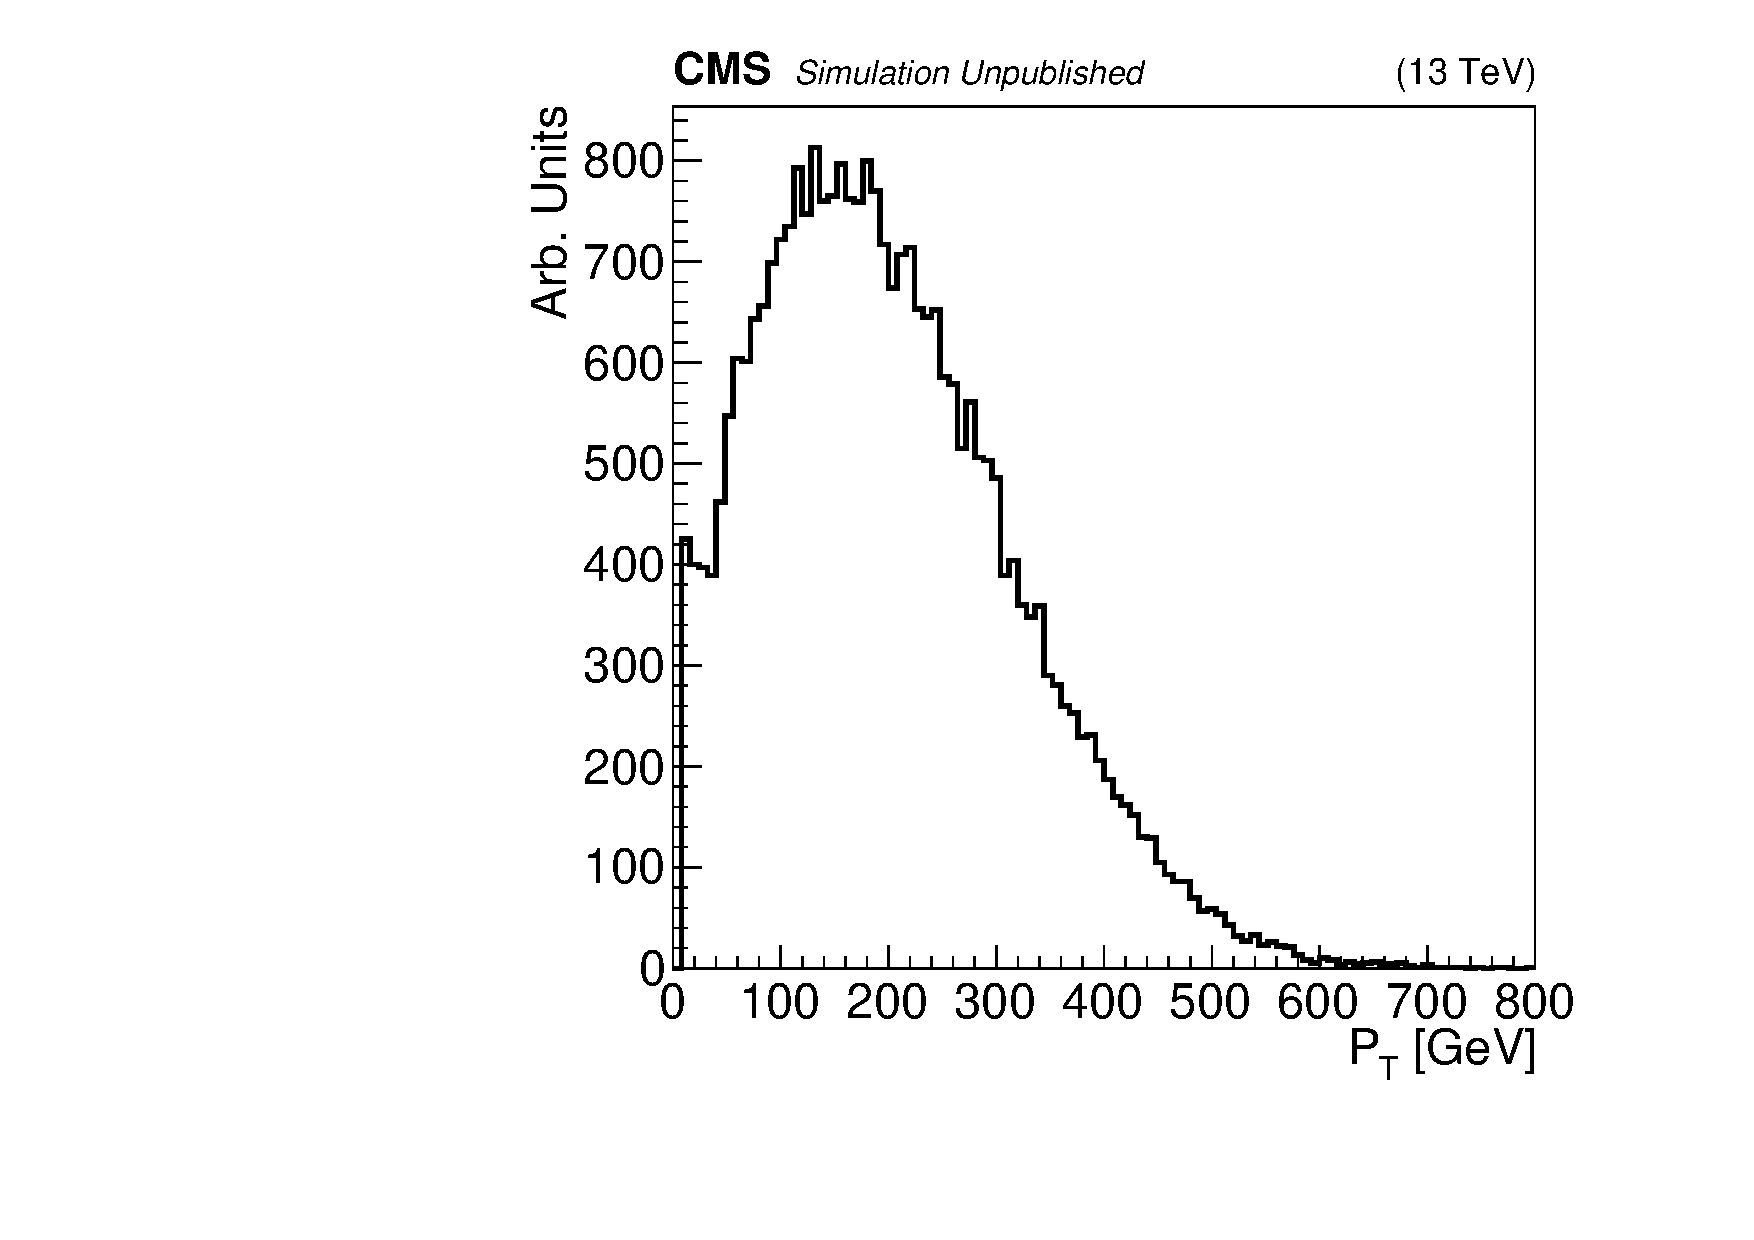
\includegraphics[width=2.4in]{figures/ptMatchedRecoJetTwo_mwr2200_mnu1100.pdf}
		\caption{jet from $\nul \rightarrow \ell jj$}\label{fig:wrLeptJetPtsd}
	\end{subfigure}
	\caption{The $\pt$ distributions of leptons and jets reconstructed in $\WR \rightarrow \ell\ell jj$ events with $\mWR = 2.2$ $\TeV$ 
		and $\mnul = \frac{1}{2}\mWR$.}\label{fig:wrLeptJetPts}
\end{figure}

\begin{figure}
	\centering
	\begin{subfigure}[t]{2.4in}
		\centering
		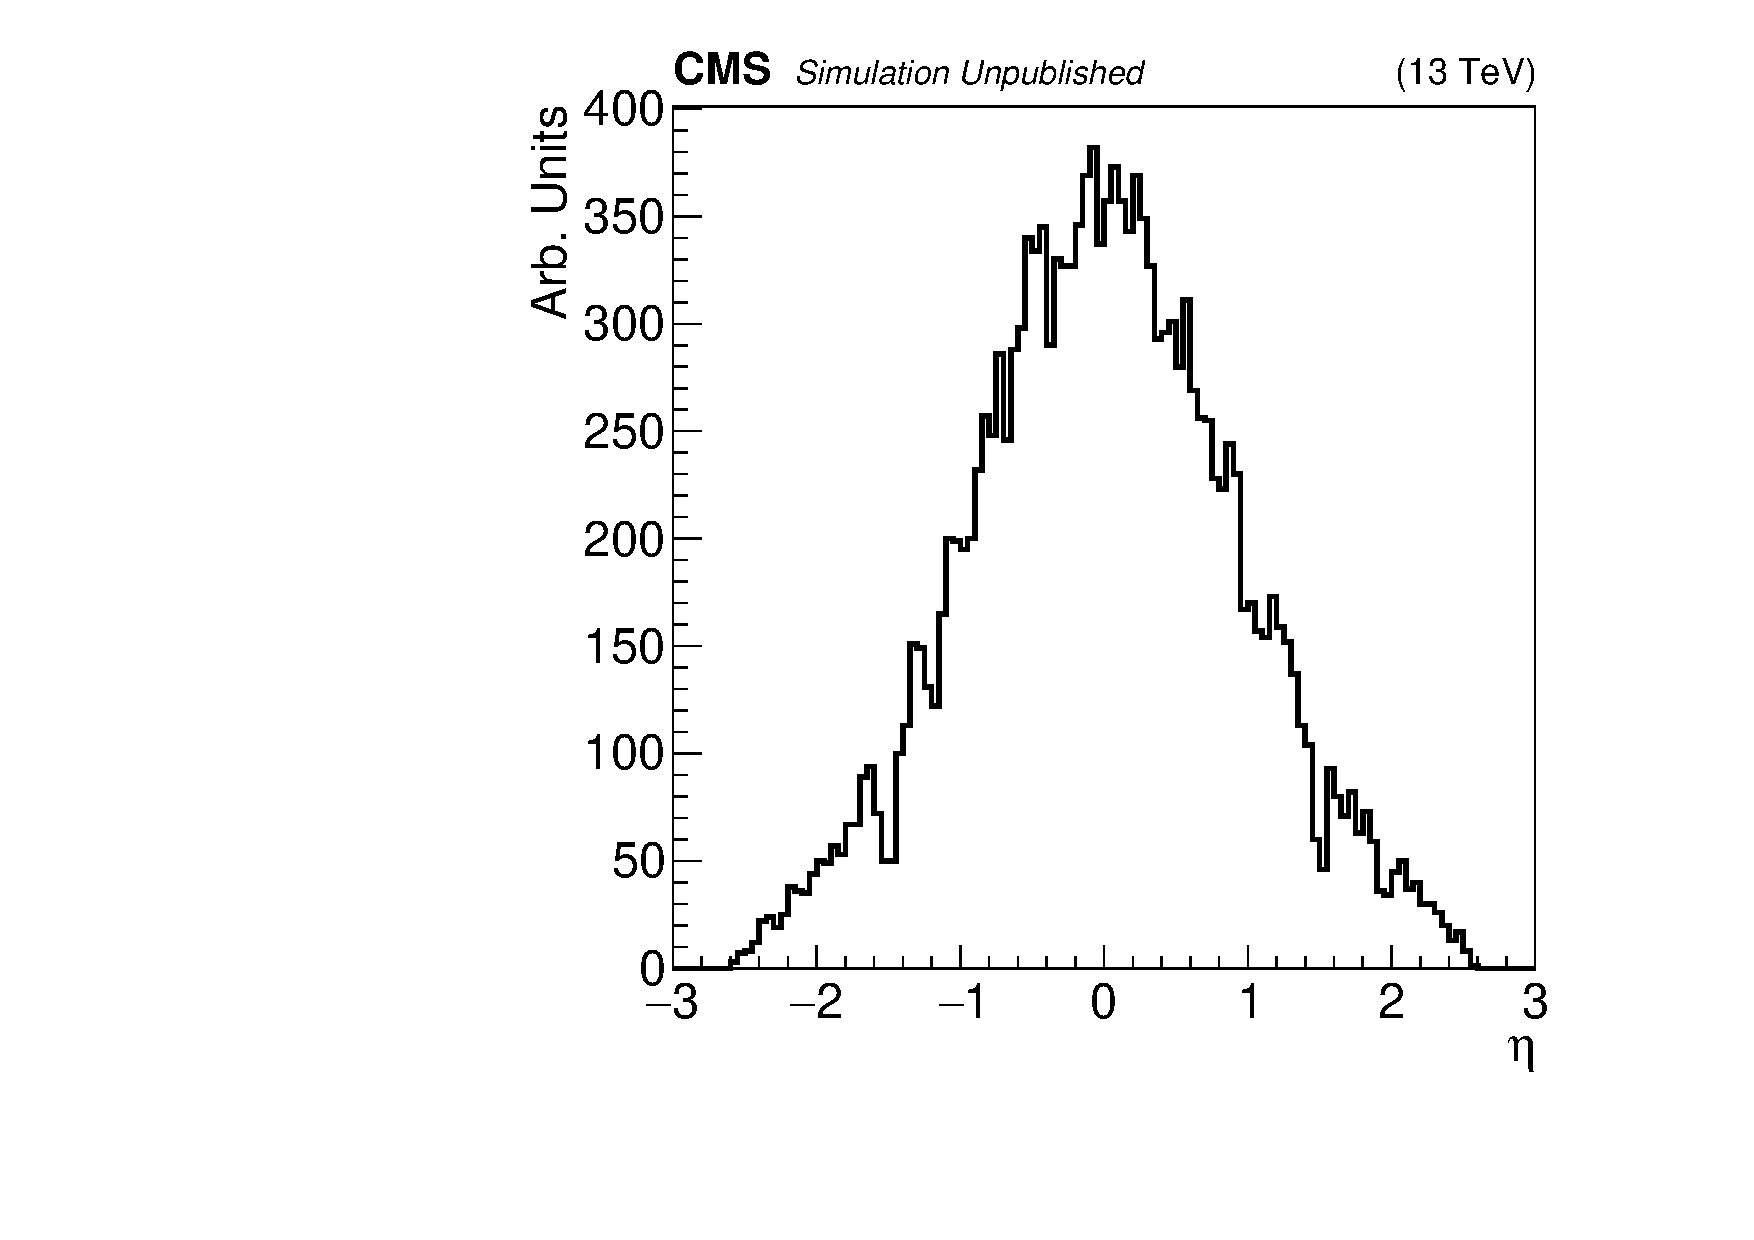
\includegraphics[width=2.4in]{figures/etaMatchedRecoEleFromWr_mwr2200_mnu1100.pdf}
		\caption{$\ell$ from $\WR \rightarrow \ell\nul$}\label{fig:wrLeptJetEtasa}
	\end{subfigure}
	\thickspace
	\begin{subfigure}[t]{2.4in}
		\centering
		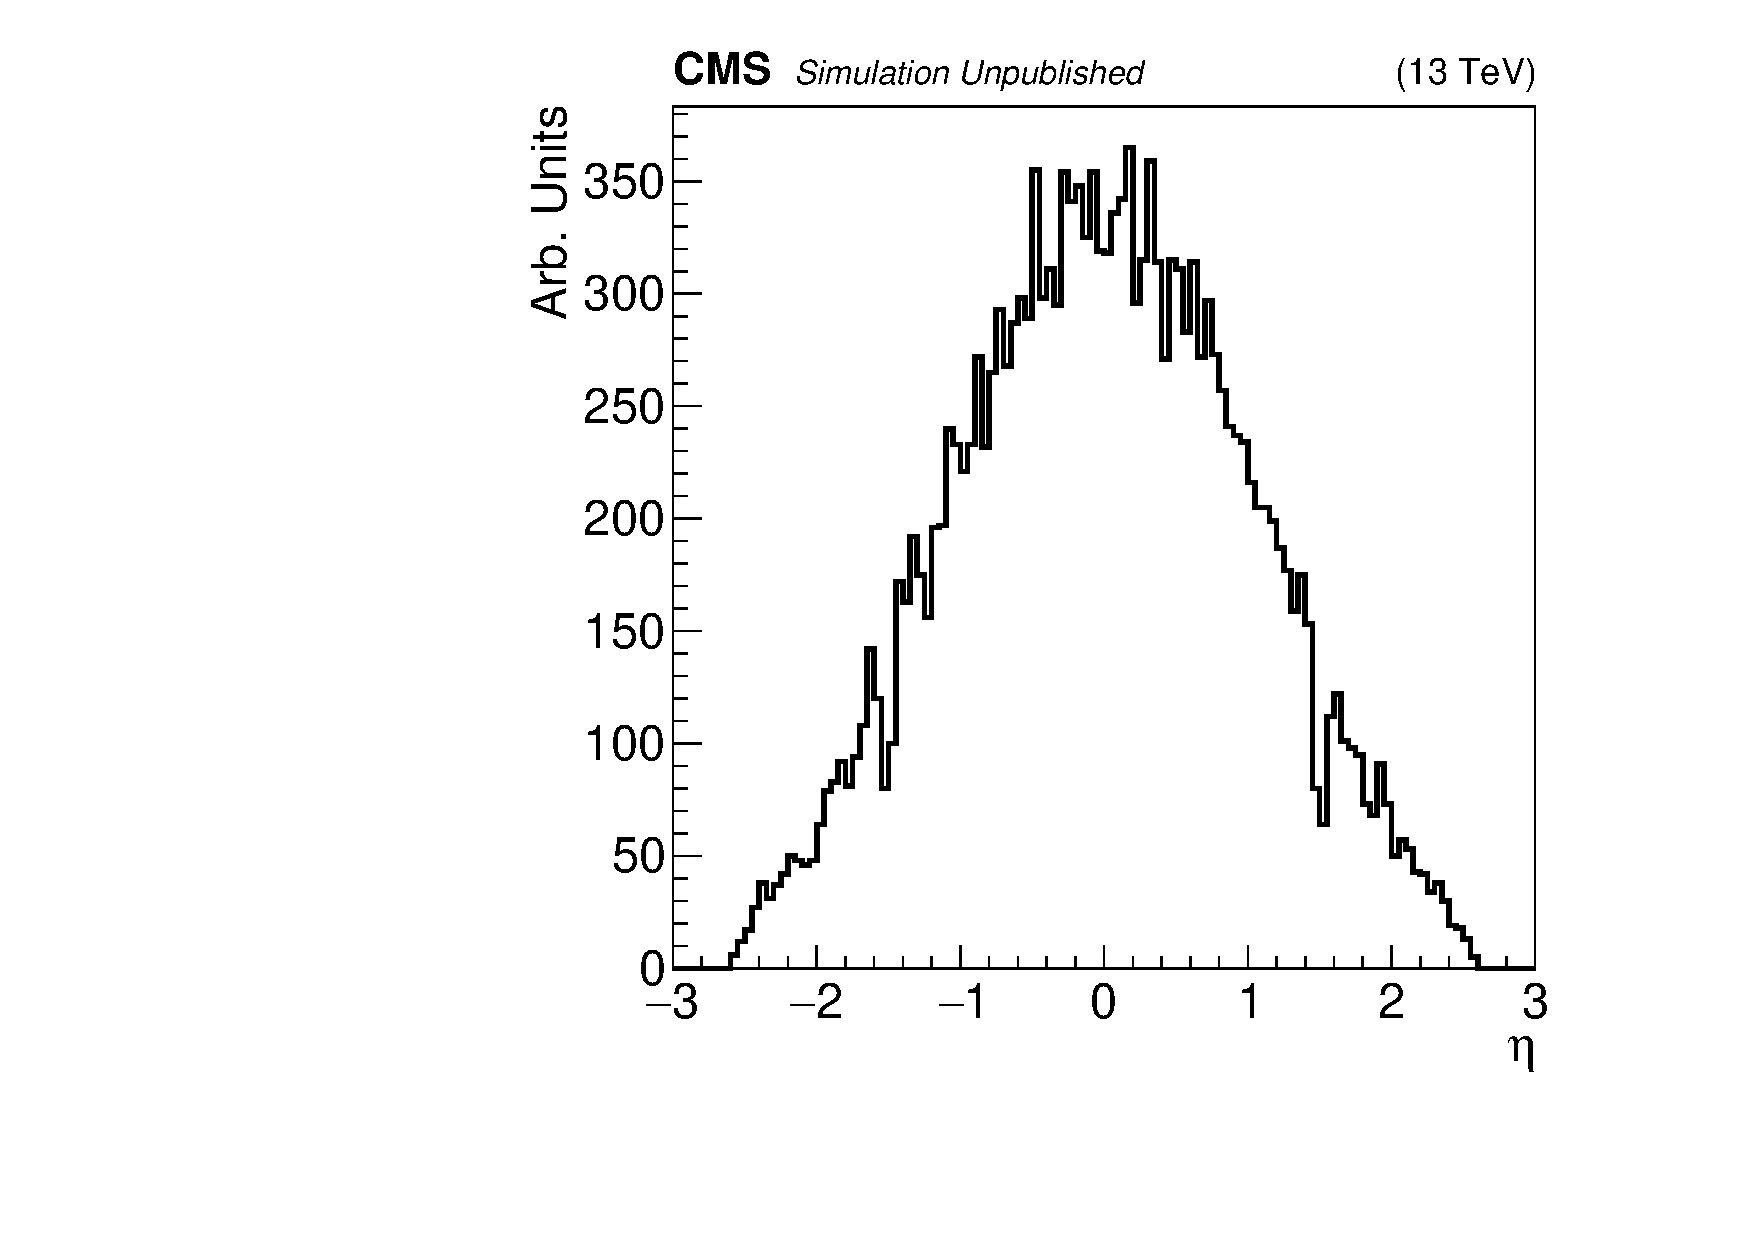
\includegraphics[width=2.4in]{figures/etaMatchedRecoEleFromNu_mwr2200_mnu1100.pdf}
		\caption{$\ell$ from $\nul \rightarrow \ell jj$}\label{fig:wrLeptJetEtasb}
	\end{subfigure}
	\newline
	\newline
	\newline
	\newline
	\begin{subfigure}[t]{2.4in}
		\centering
		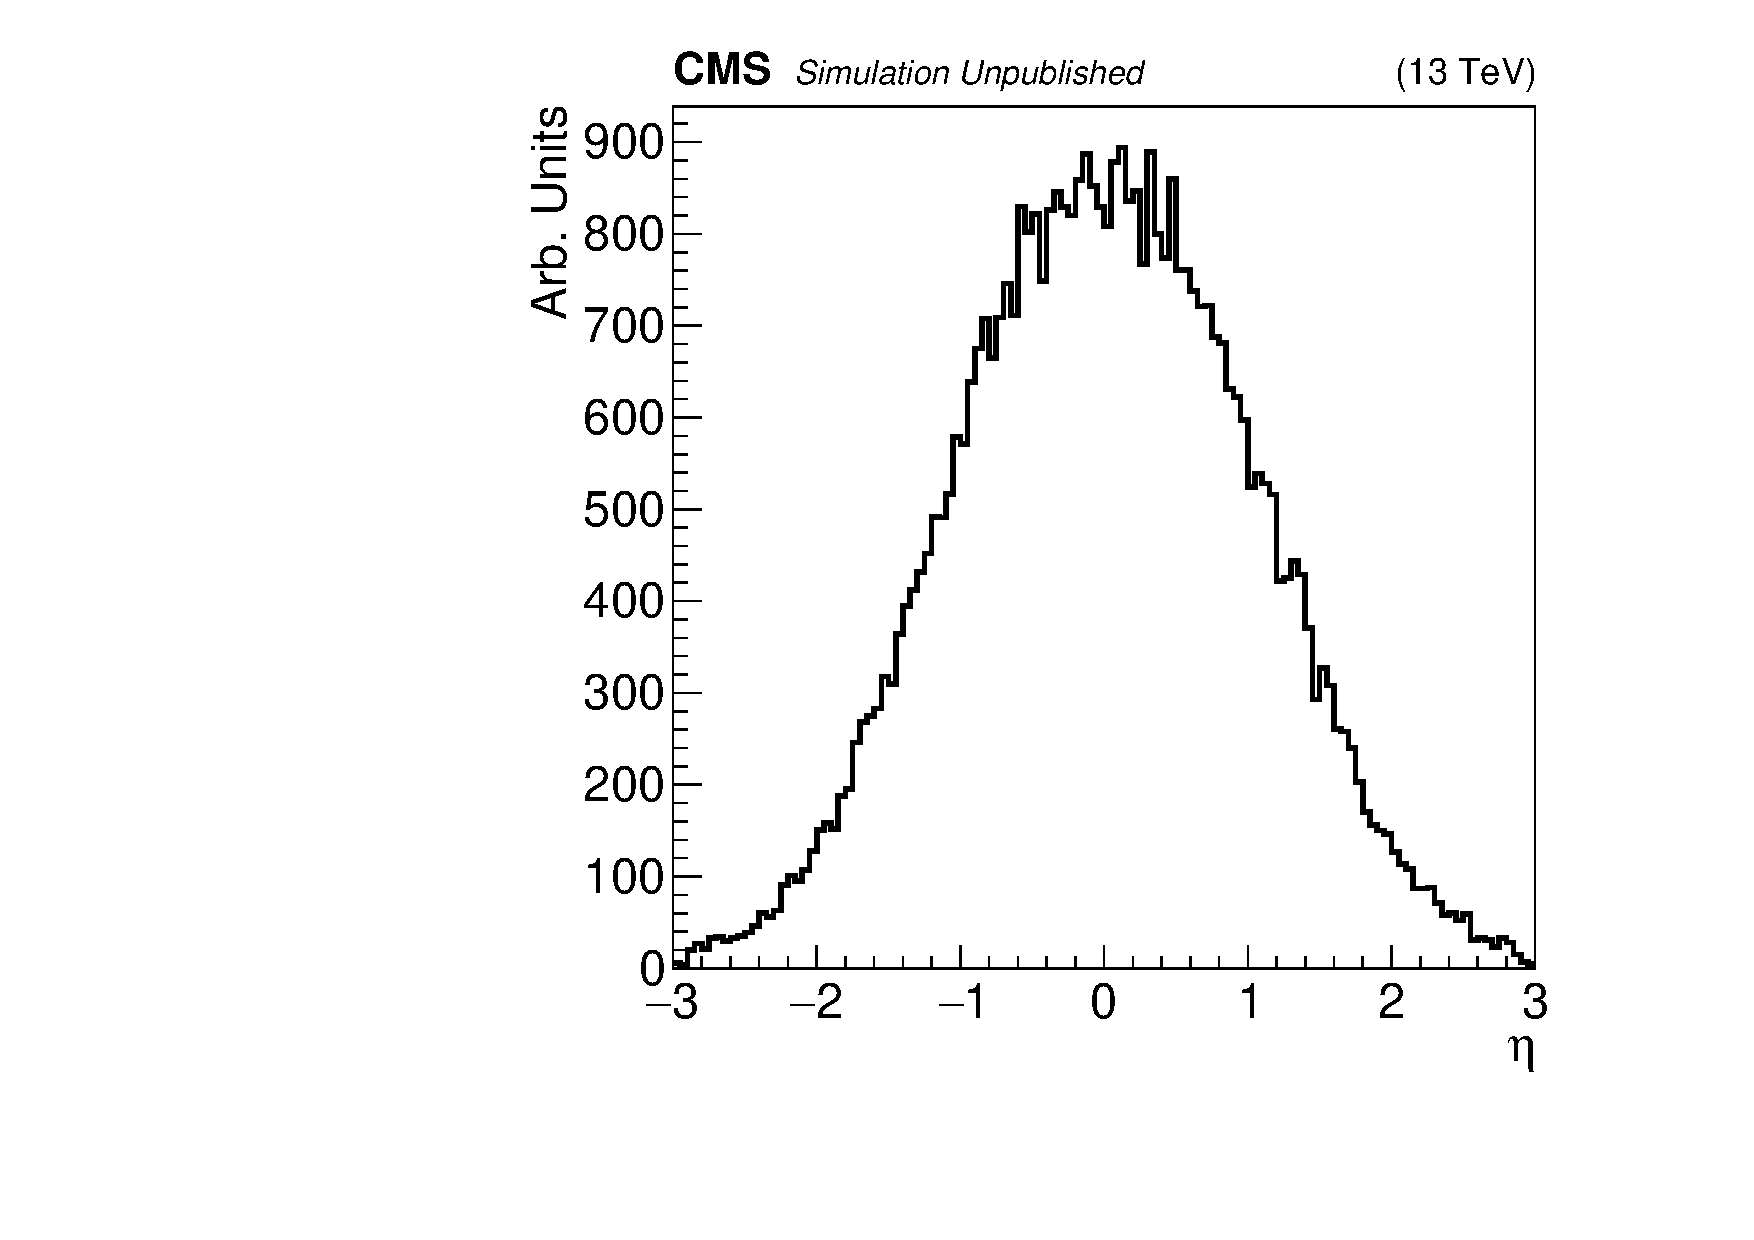
\includegraphics[width=2.4in]{figures/etaMatchedRecoJetOne_mwr2200_mnu1100.pdf}
		\caption{jet from $\nul \rightarrow \ell jj$}\label{fig:wrLeptJetEtasc}
	\end{subfigure}
	\thickspace
	\begin{subfigure}[t]{2.4in}
		\centering
		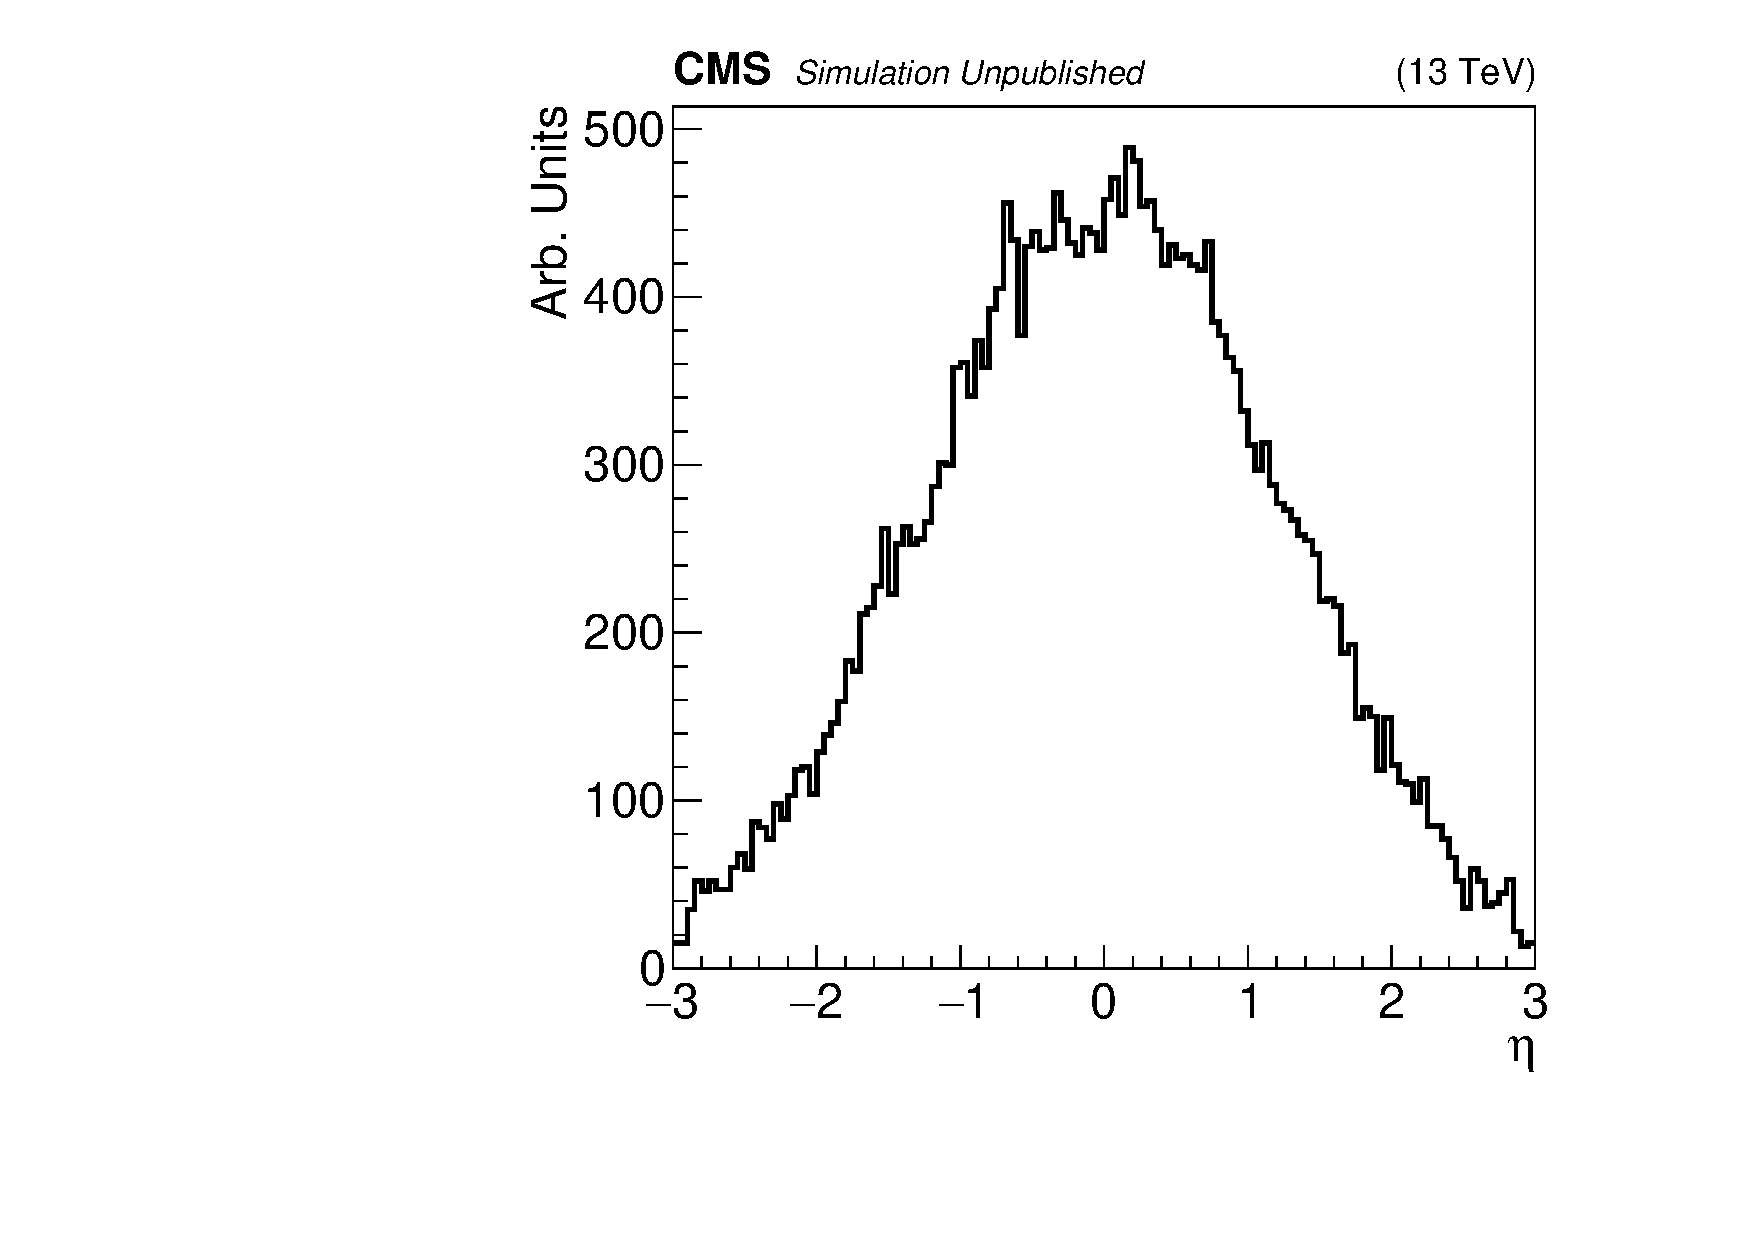
\includegraphics[width=2.4in]{figures/etaMatchedRecoJetTwo_mwr2200_mnu1100.pdf}
		\caption{jet from $\nul \rightarrow \ell jj$}\label{fig:wrLeptJetEtasd}
	\end{subfigure}
	\caption{The $\eta$ distributions of leptons and jets reconstructed in $\WR \rightarrow \ell\ell jj$ events with $\mWR = 2.2$ $\TeV$ 
		and $\mnul = \frac{1}{2}\mWR$.}\label{fig:wrLeptJetEtas}
\end{figure}

\begin{figure}
	\centering
	\begin{subfigure}[t]{2.4in}
		\centering
		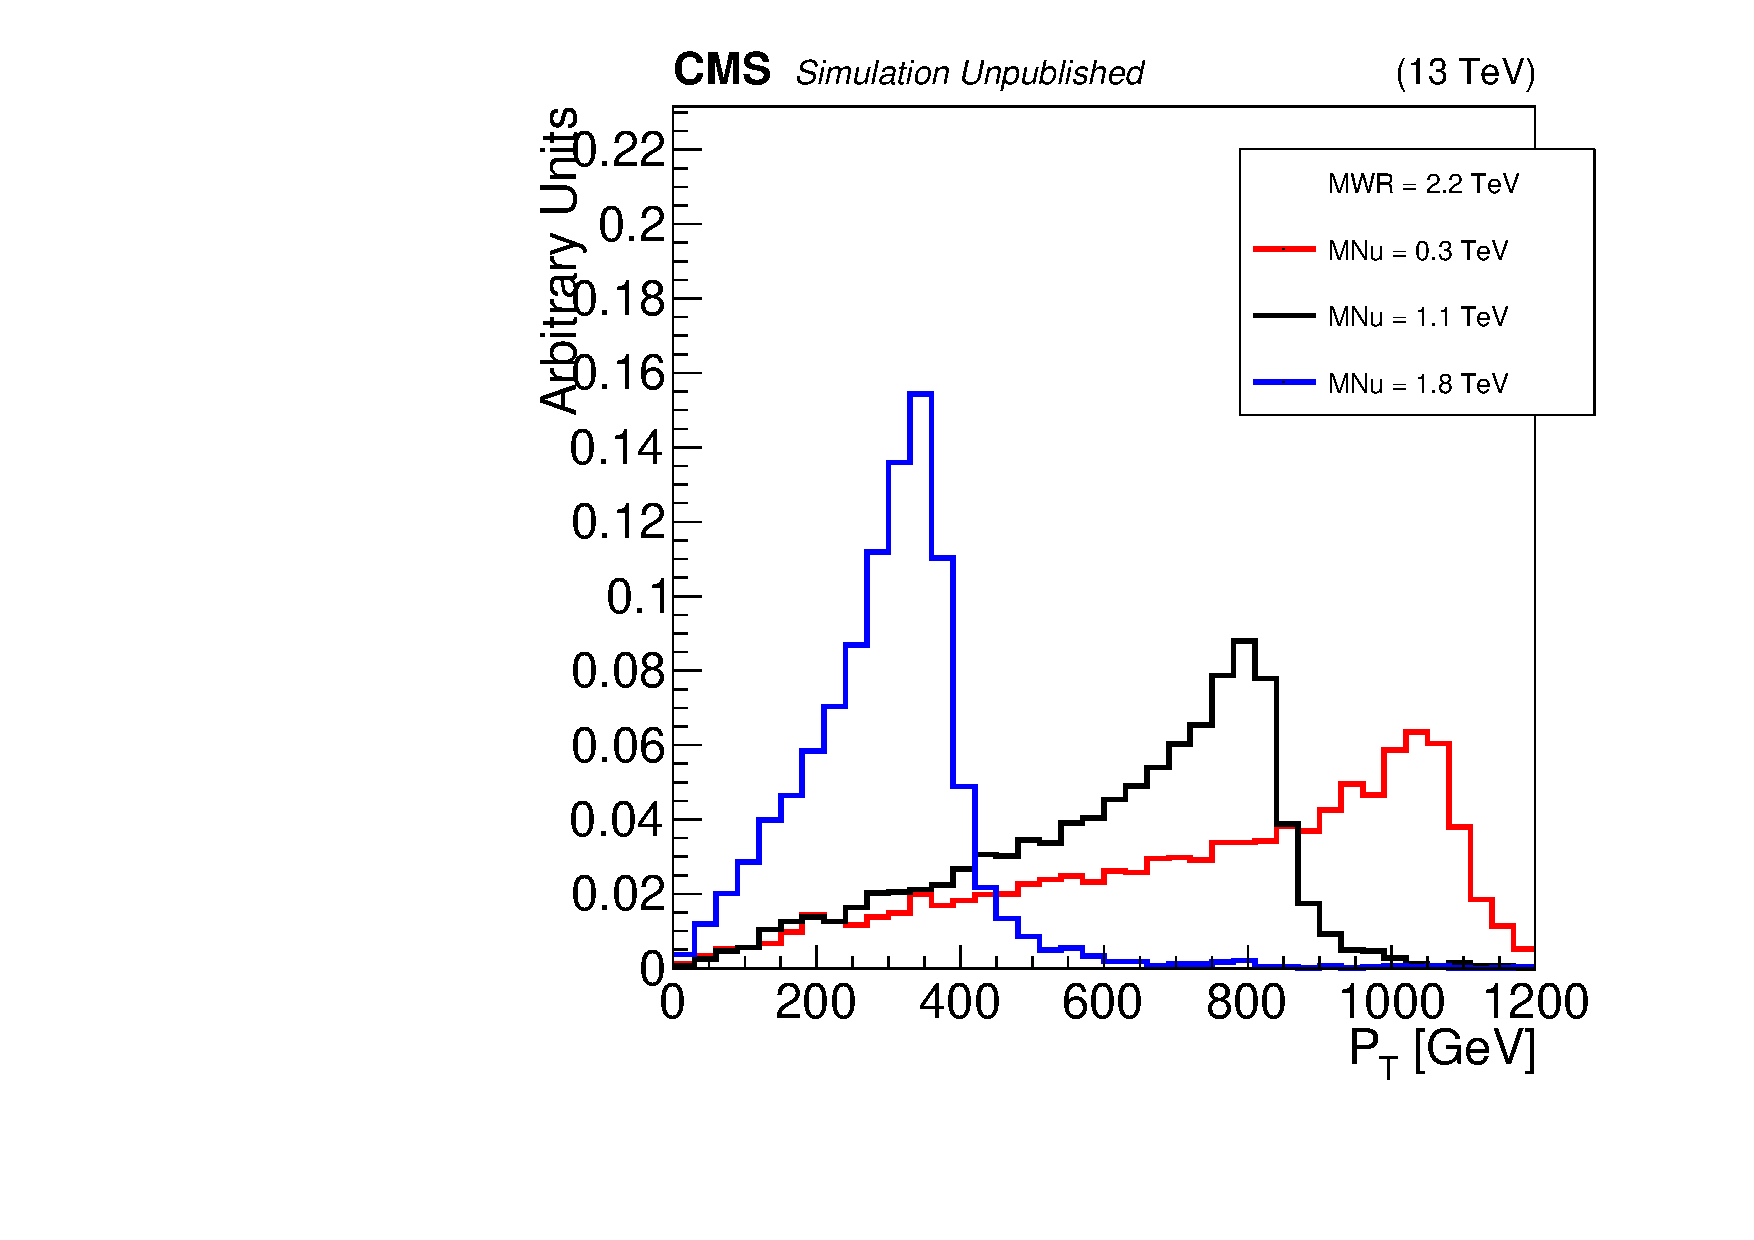
\includegraphics[width=2.4in]{figures/ptGenLeptFromFstHvyPtcl_MWR_2200_several_MNu_private.pdf}
		\caption{$\ell$ from $\WR \rightarrow \ell\nul$}\label{fig:wrLeptQrkPtsVarMNua}
	\end{subfigure}
	\thickspace
	\begin{subfigure}[t]{2.4in}
		\centering
		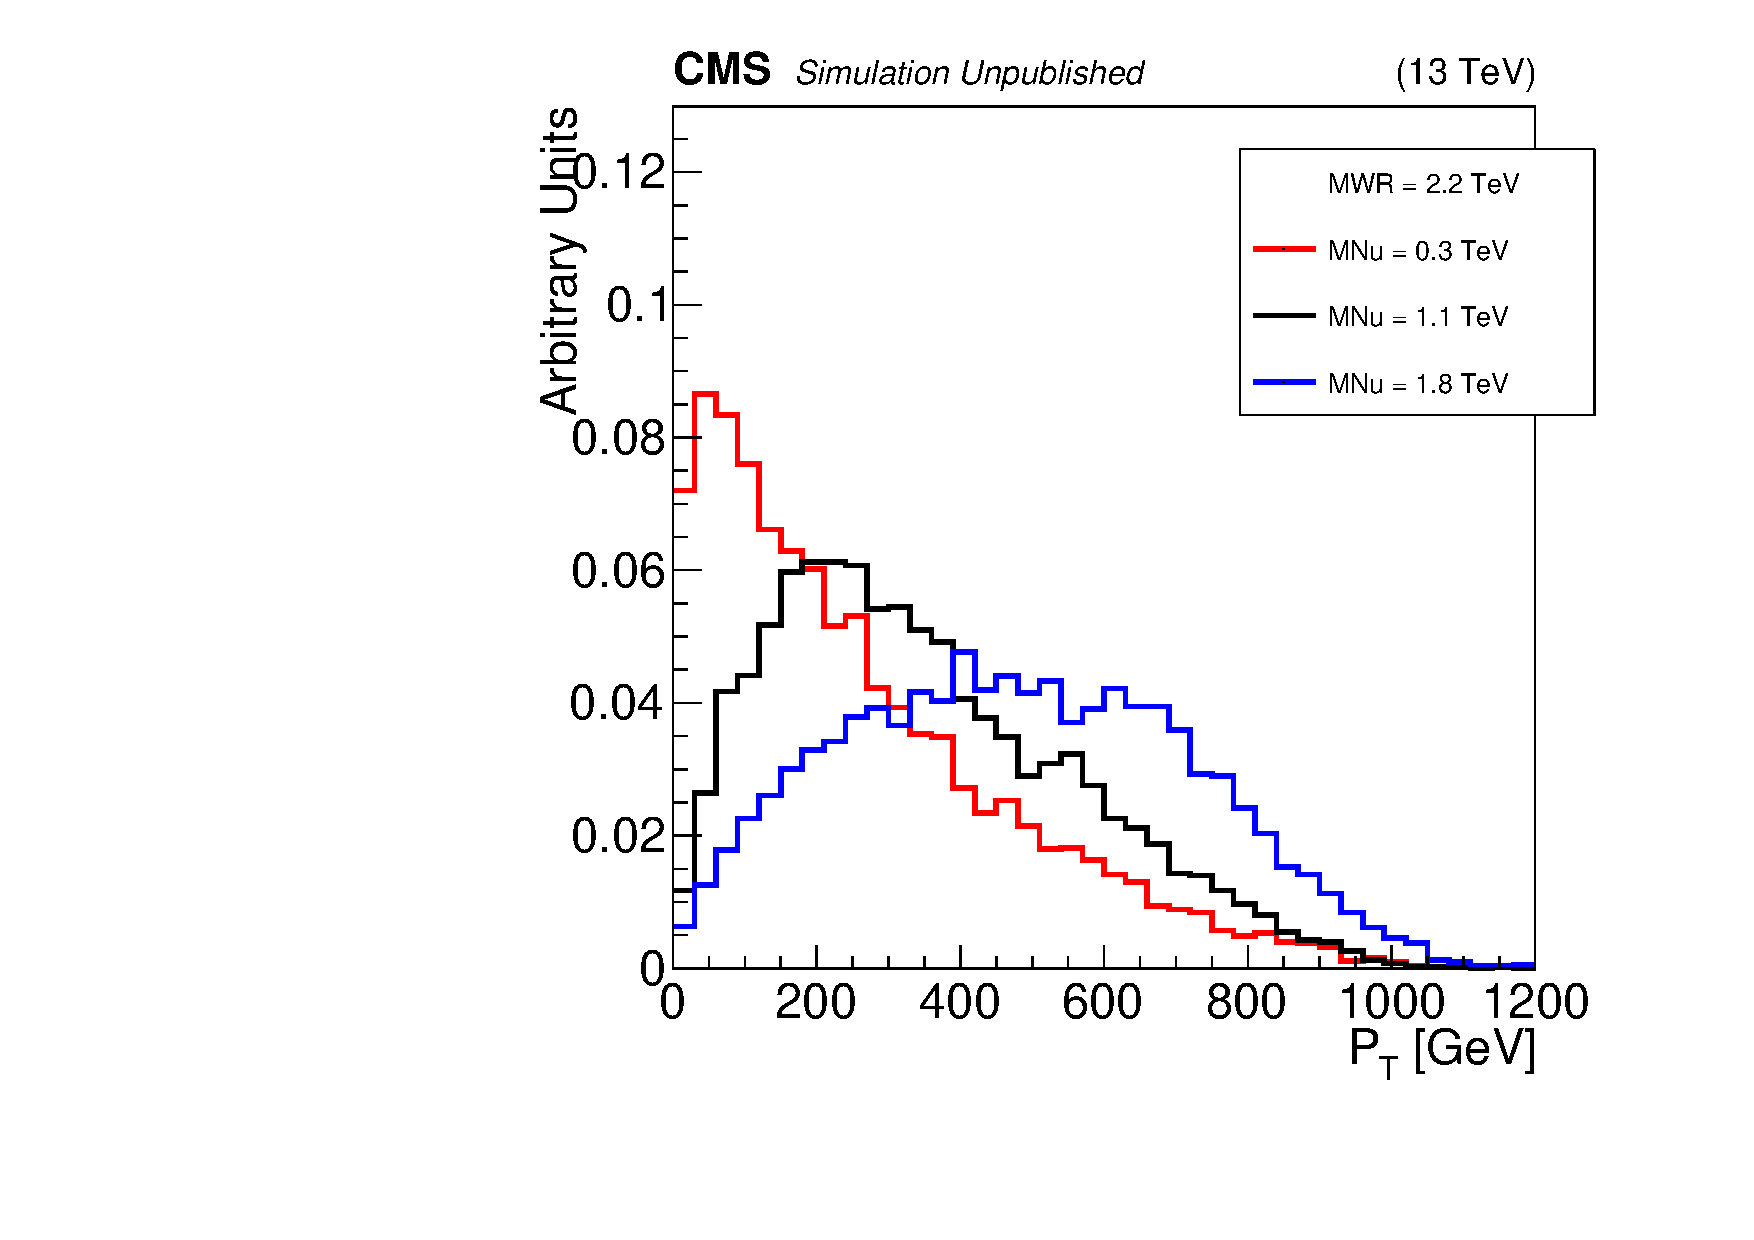
\includegraphics[width=2.4in]{figures/ptGenLeptFromScdHvyPtcl_MWR_2200_several_MNu_private.pdf}
		\caption{$\ell$ from $\nul \rightarrow \ell qq$}\label{fig:wrLeptQrkPtsVarMNub}
	\end{subfigure}
	\newline
	\newline
	\newline
	\newline
	\begin{subfigure}[t]{2.4in}
		\centering
		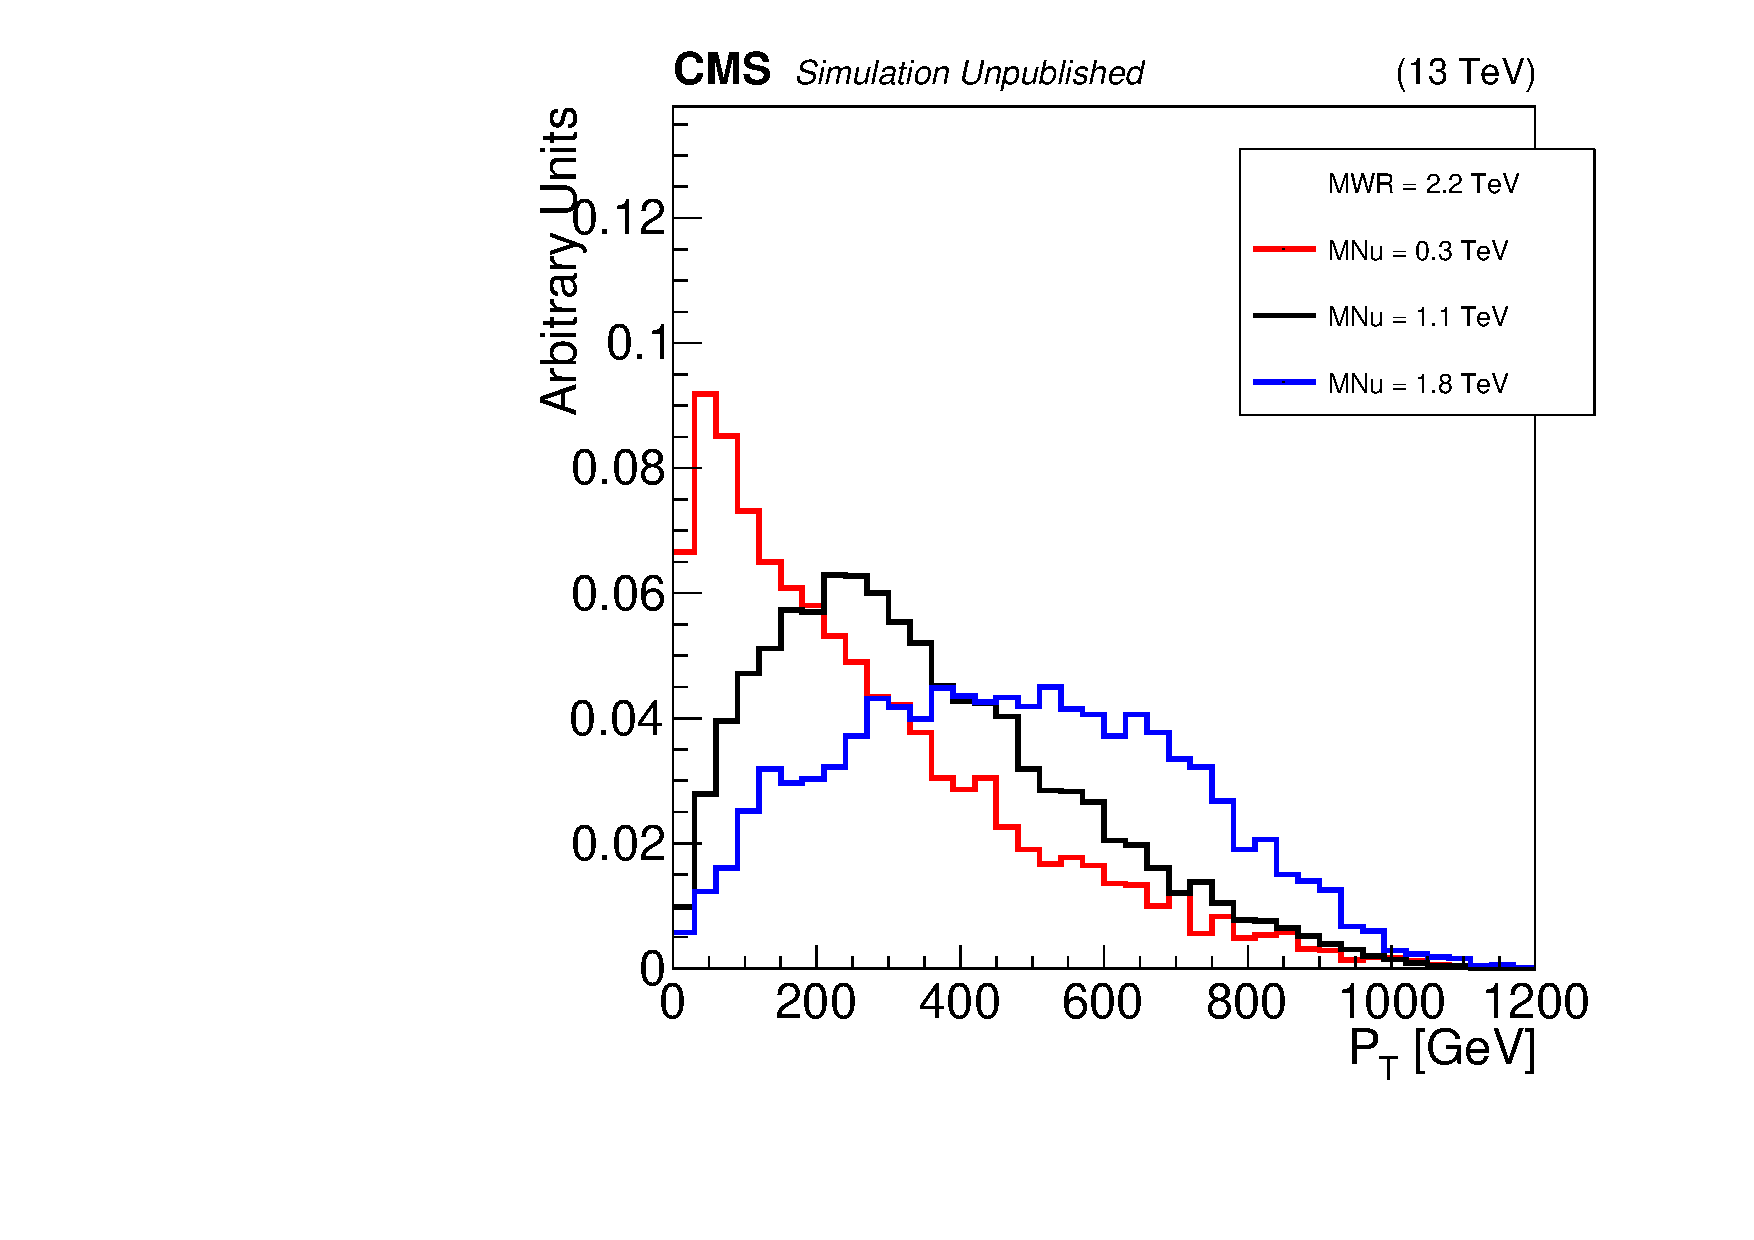
\includegraphics[width=2.4in]{figures/ptGenQuarkOneFromScdHvyPtcl_MWR_2200_several_MNu_private.pdf}
		\caption{quark from $\nul \rightarrow \ell qq$}\label{fig:wrLeptQrkPtsVarMNuc}
	\end{subfigure}
	\thickspace
	\begin{subfigure}[t]{2.4in}
		\centering
		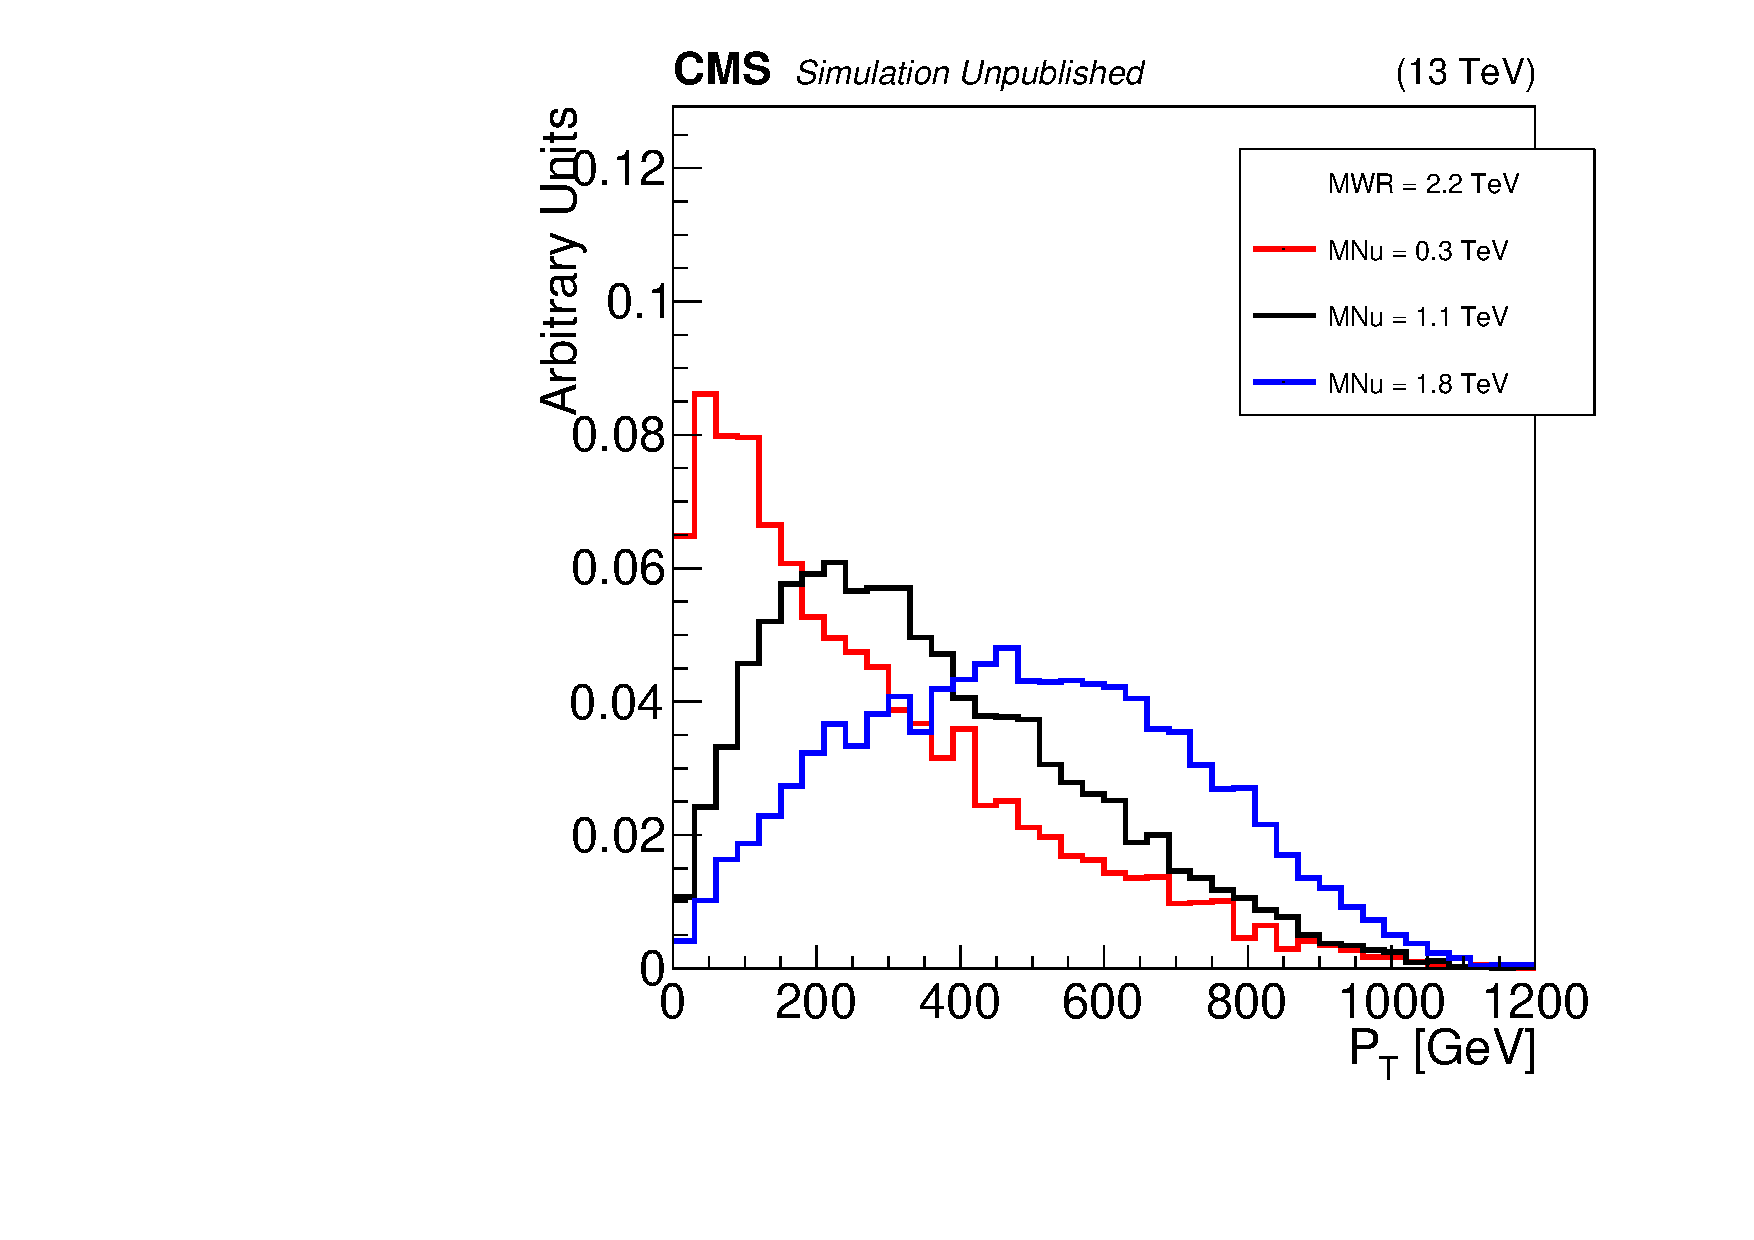
\includegraphics[width=2.4in]{figures/ptGenQuarkTwoFromScdHvyPtcl_MWR_2200_several_MNu_private.pdf}
		\caption{quark from $\nul \rightarrow \ell qq$}\label{fig:wrLeptQrkPtsVarMNud}
	\end{subfigure}
	\caption{The $\pt$ distributions of leptons and quarks produced in $\WR \rightarrow \ell\ell qq$ events with $\mWR = 2.2$ $\TeV$ 
		and different \mnul.}\label{fig:wrLeptQrkPtsVarMNu}
\end{figure}

\begin{figure}[h]
	\centering
	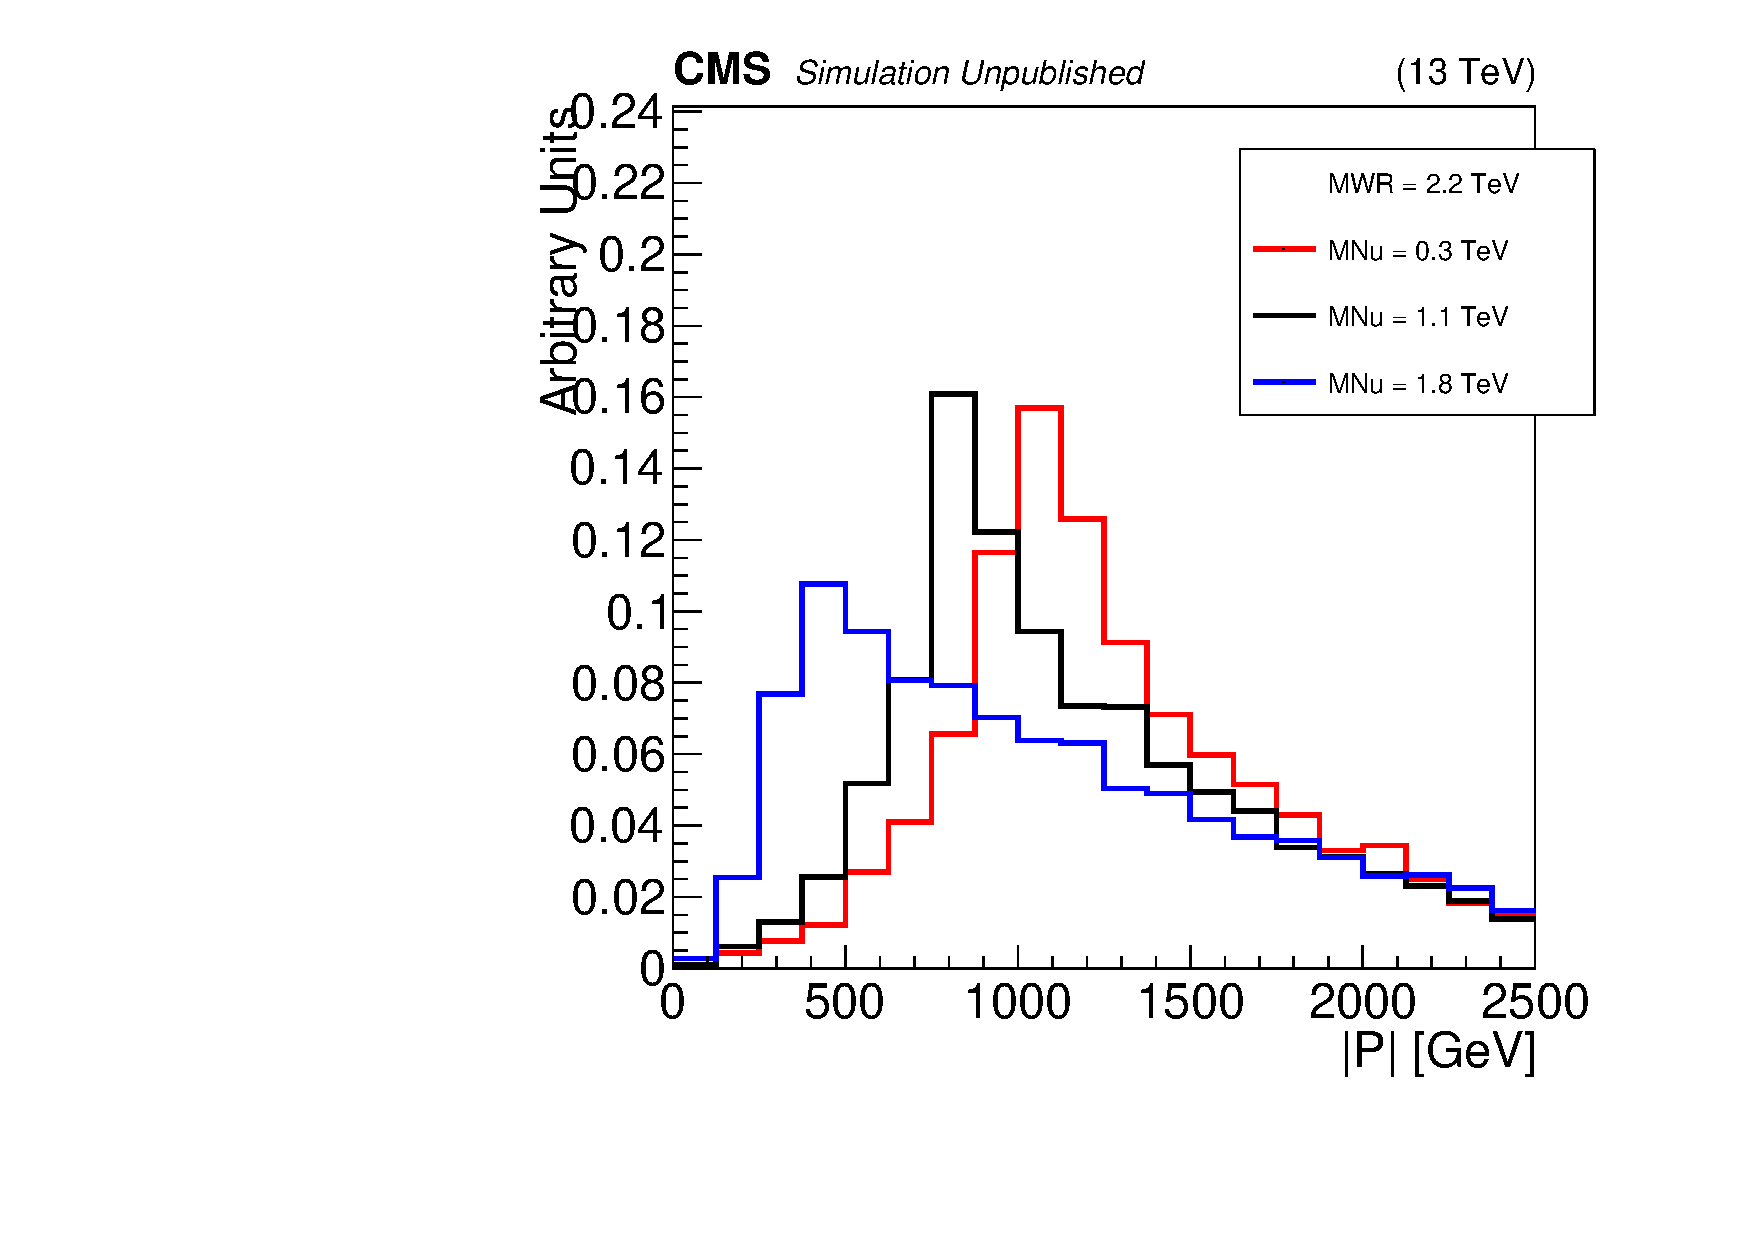
\includegraphics[width=0.5\textwidth]{figures/genNuMomMag_MWR_2200_several_MNu_private.pdf}
	\caption{The $|p|$ distribution of the \nul produced in $\WR \rightarrow \ell\nul$ events with $\mWR = 2.2$ $\TeV$ and different \mnul.}
	\label{fig:hvyNuMomentumVarMNu}
\end{figure}

\begin{figure}
	\centering
	\begin{subfigure}[t]{2.4in}
		\centering
		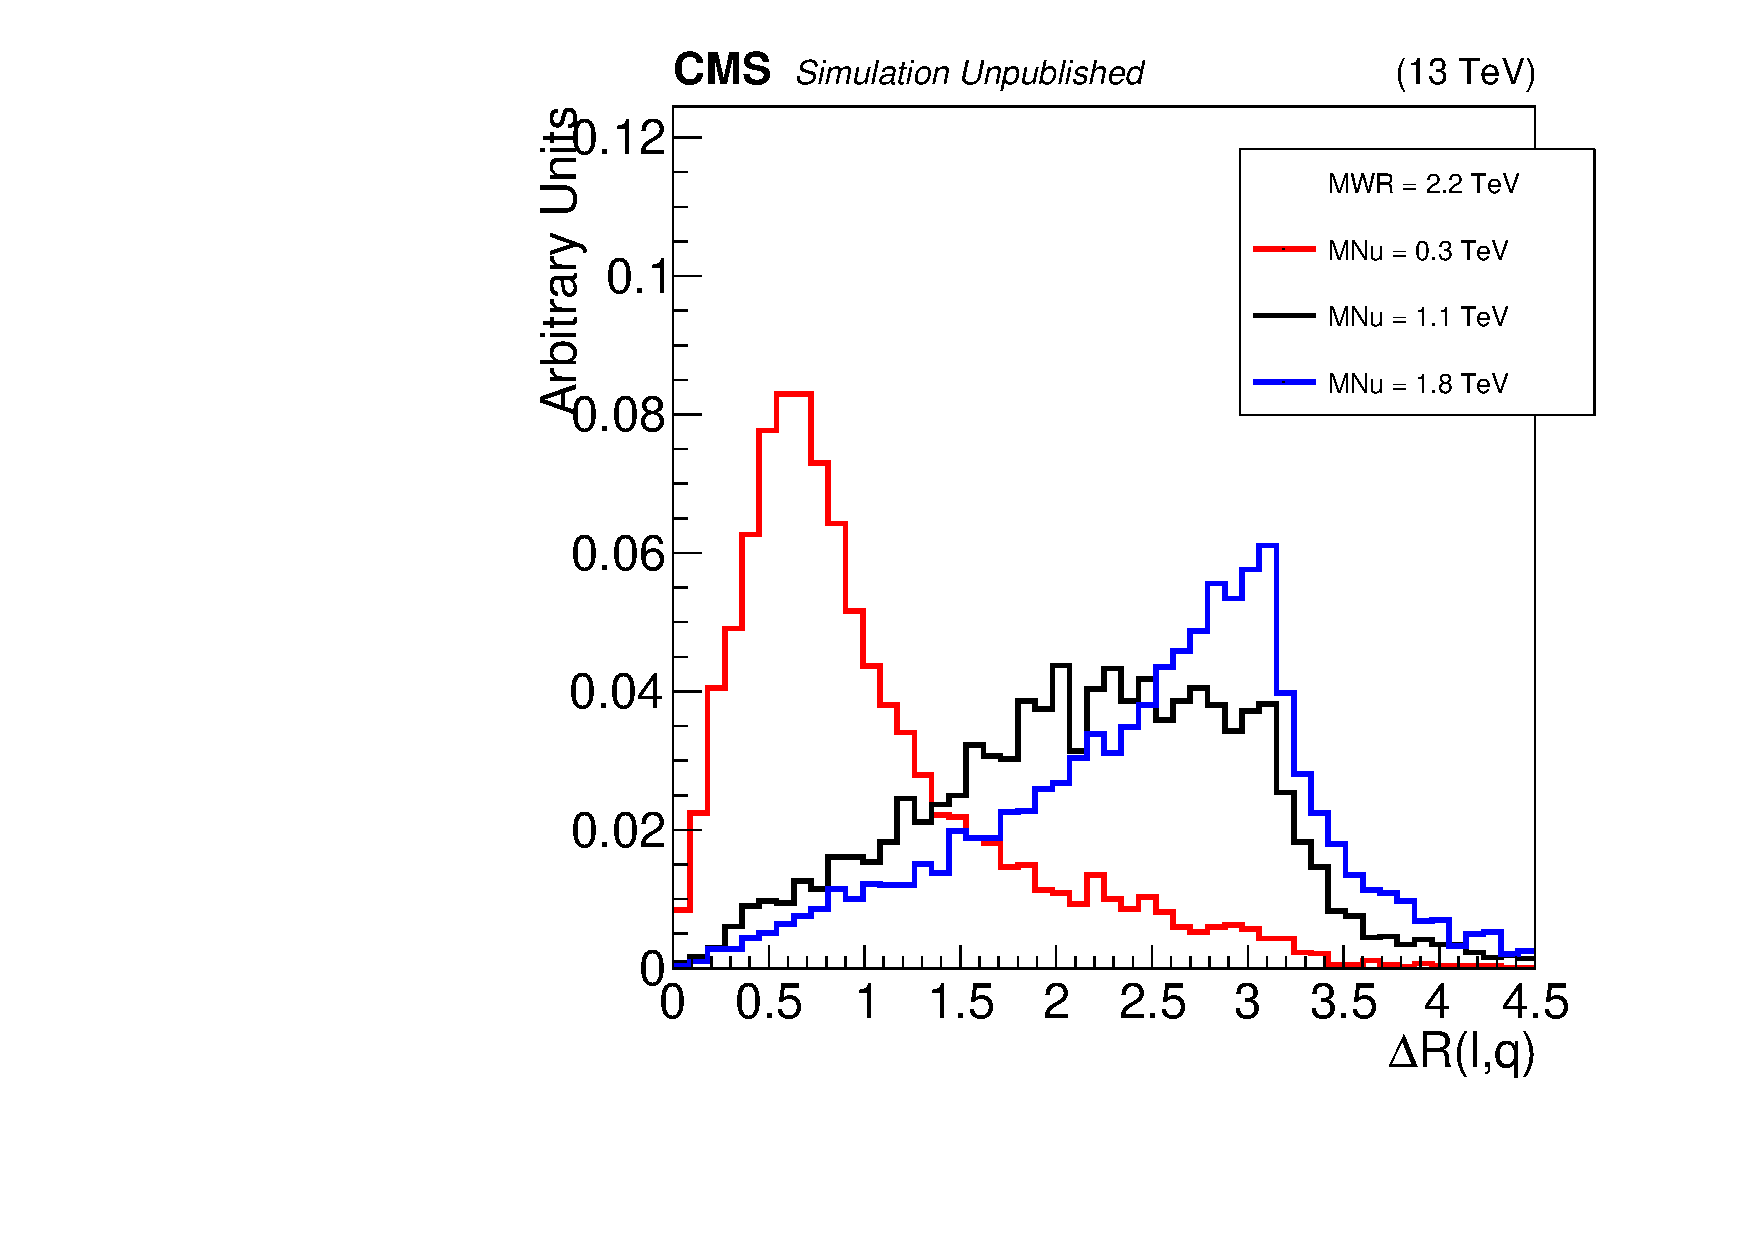
\includegraphics[width=2.4in]{figures/dRgenLeptonFromScdHvyPtclGenQuarkOneFromScdHvyPtcl_MWR_2200_several_MNu_private.pdf}
		%\caption{ }\label{fig:wrDrLeptQrkVarMNua}
	\end{subfigure}
	\thickspace
	\begin{subfigure}[t]{2.4in}
		\centering
		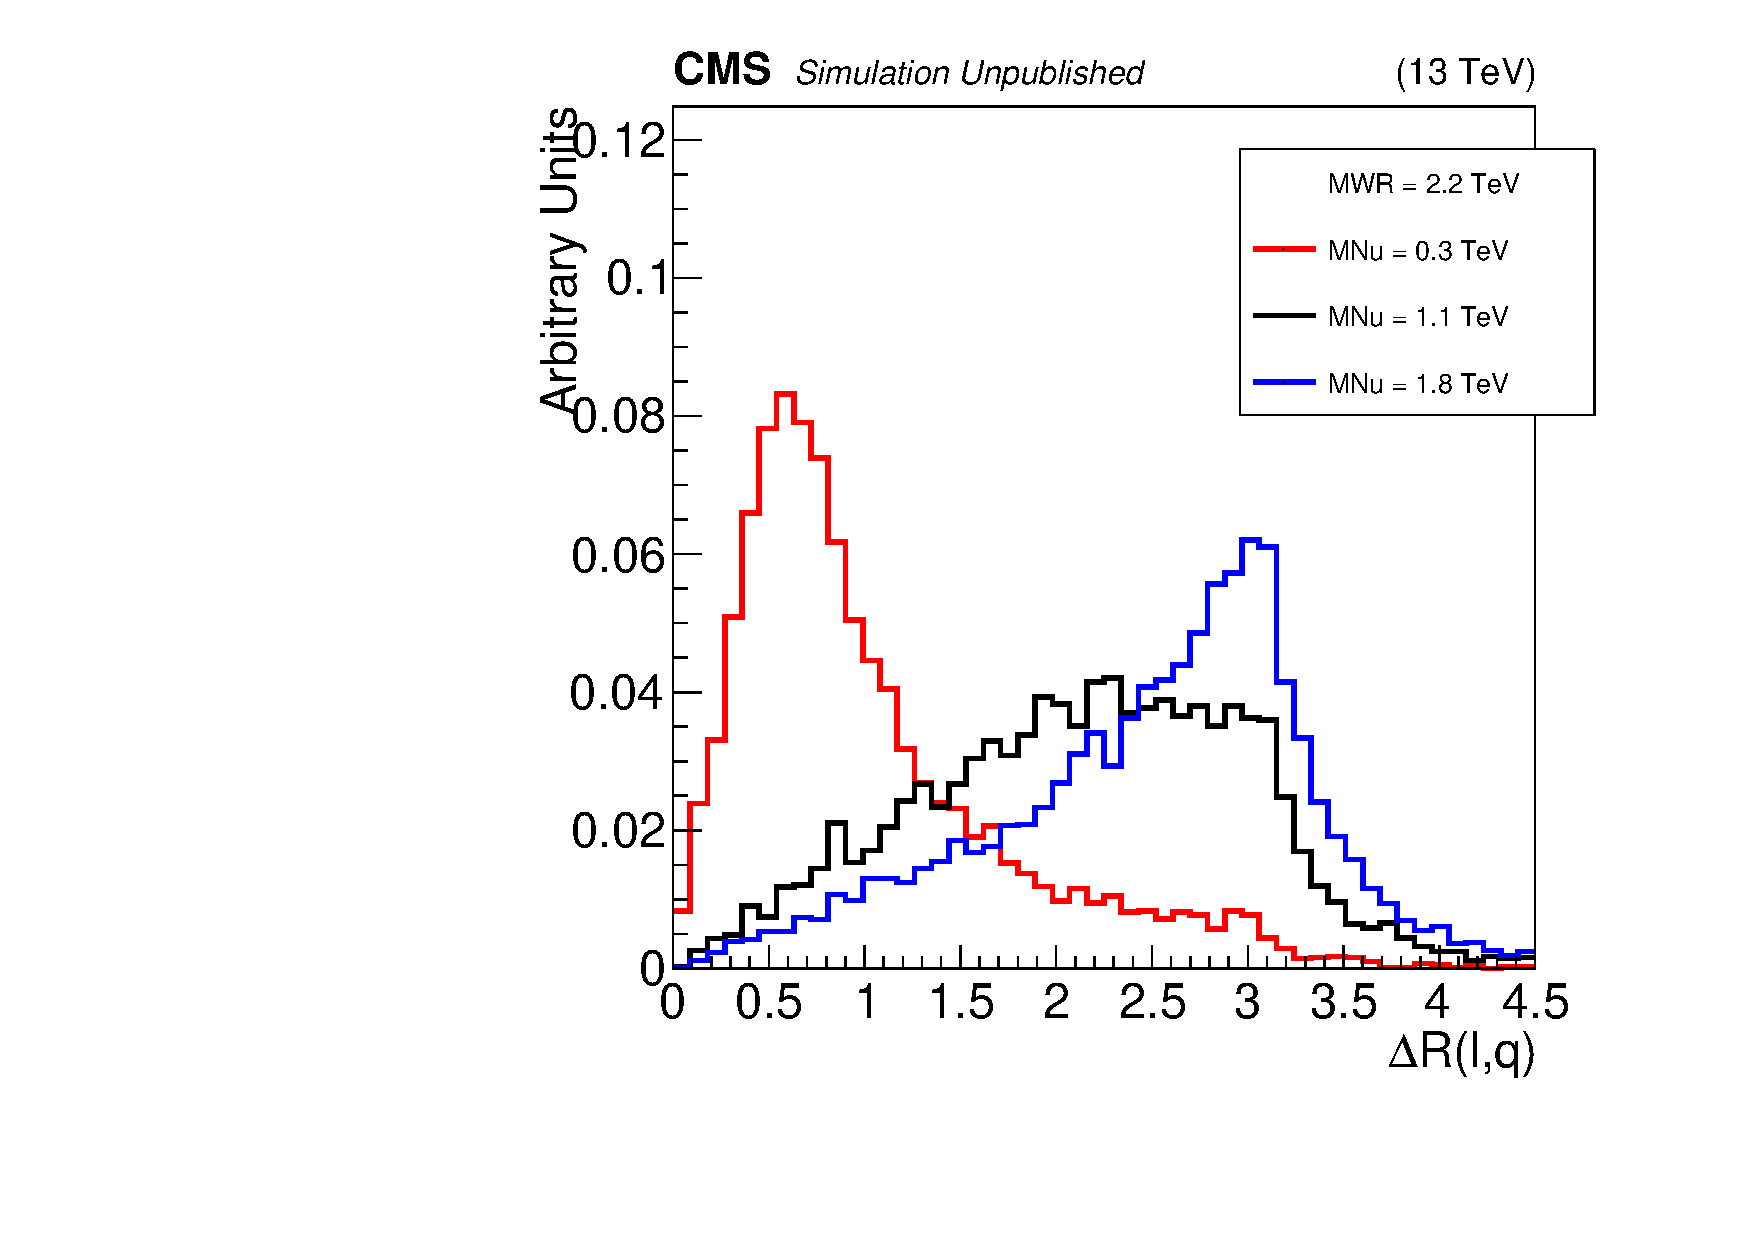
\includegraphics[width=2.4in]{figures/dRgenLeptonFromScdHvyPtclGenQuarkTwoFromScdHvyPtcl_MWR_2200_several_MNu_private.pdf}
		%\caption{ }\label{fig:wrDrLeptQrkVarMNub}
	\end{subfigure}
	\caption{The $\Delta R(\ell,q)$ separation distributions between the $\ell$ and both quarks produced in $\nul \rightarrow \ell qq$ 
		in $\WR \rightarrow \ell\ell qq$ events with $\mWR = 2.2$ $\TeV$ and different \mnul.}\label{fig:wrDrLeptQrkVarMNu}
\end{figure}

\begin{figure}[h]
	\centering
	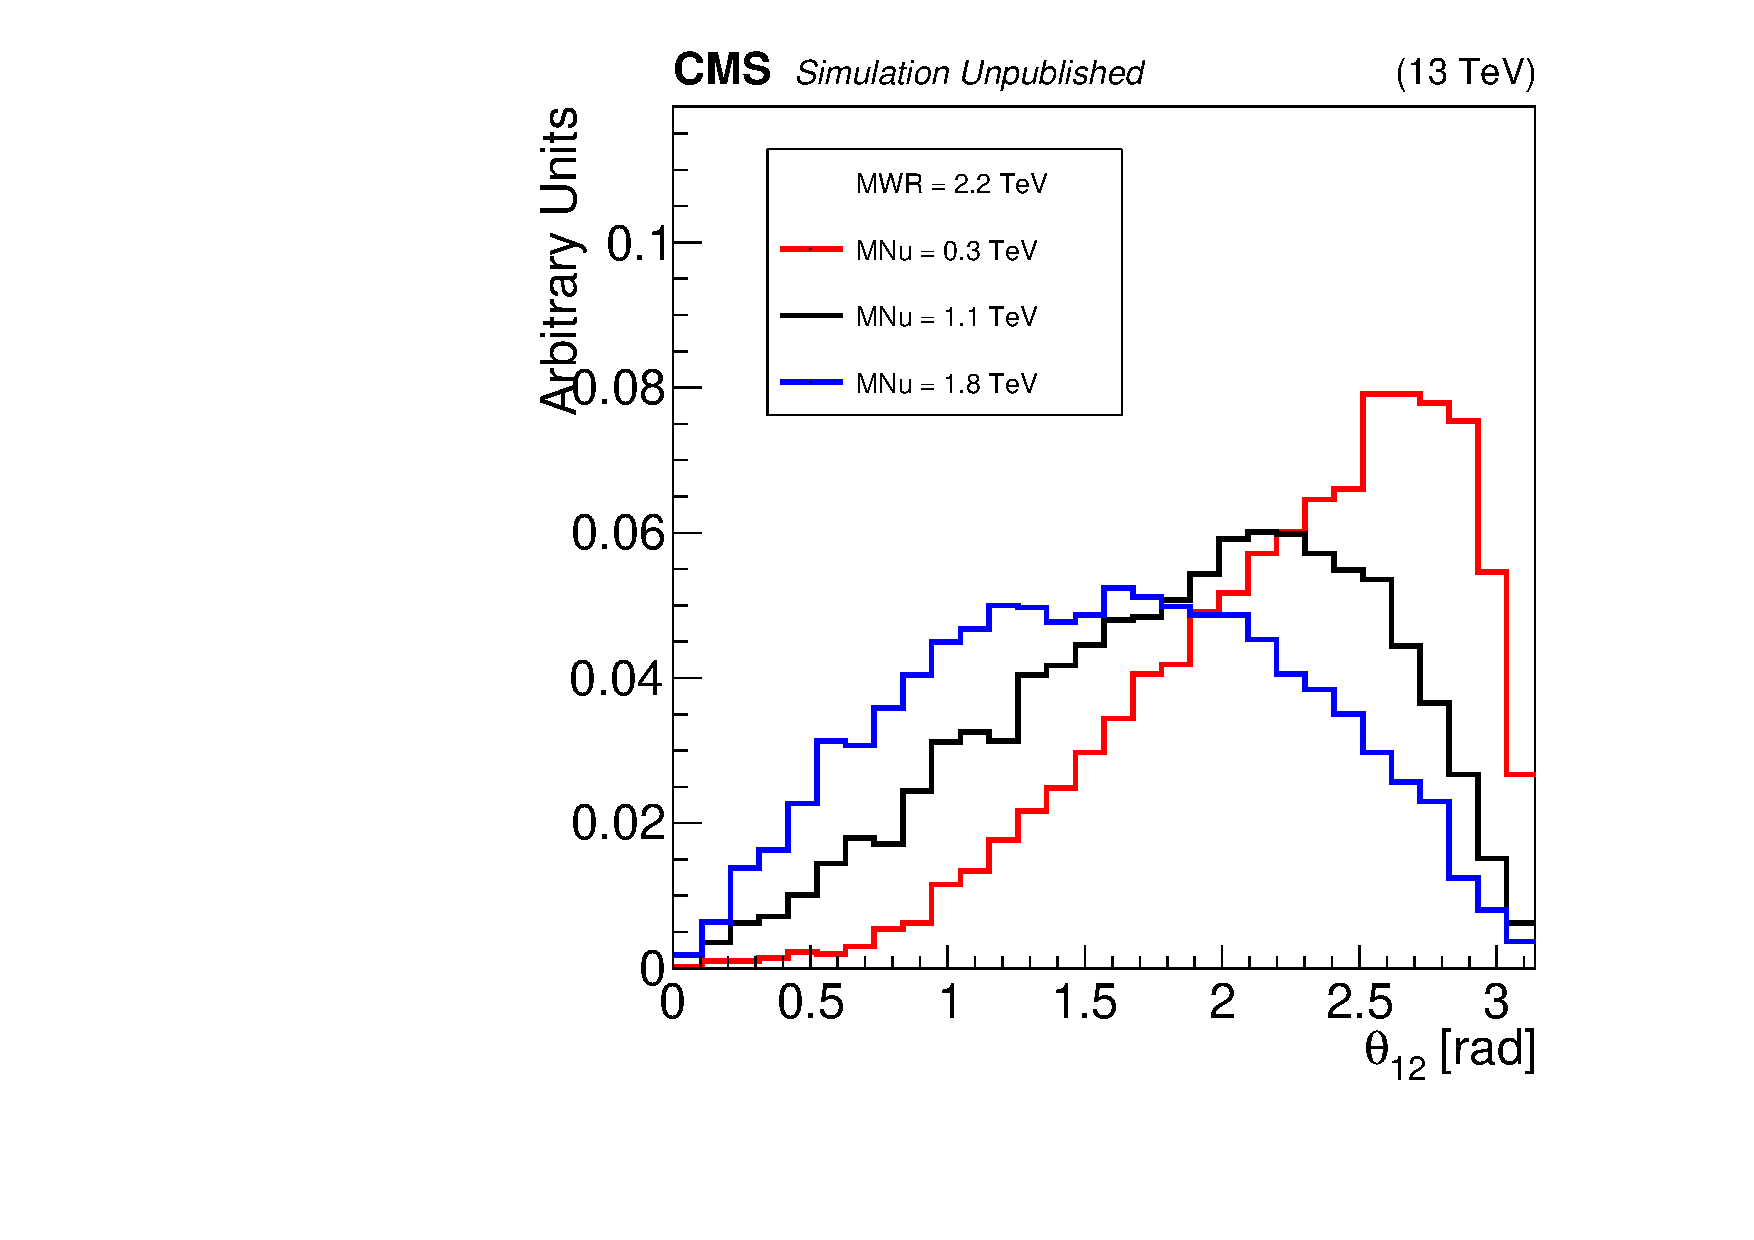
\includegraphics[width=0.5\textwidth]{figures/angleBtwnGenLepts_MWR_2200_several_MNu_private.pdf}
	\caption{The distribution of the angle $\theta_{12}$ between the two leptons produced in $\WR \rightarrow \ell_{1}\ell_{2} qq$ events with 
		$\mWR = 2.2$ $\TeV$ and different \mnul.}
	\label{fig:wrLeptAngleSepVarMNu}
\end{figure}

\begin{figure}[h]
	\centering
	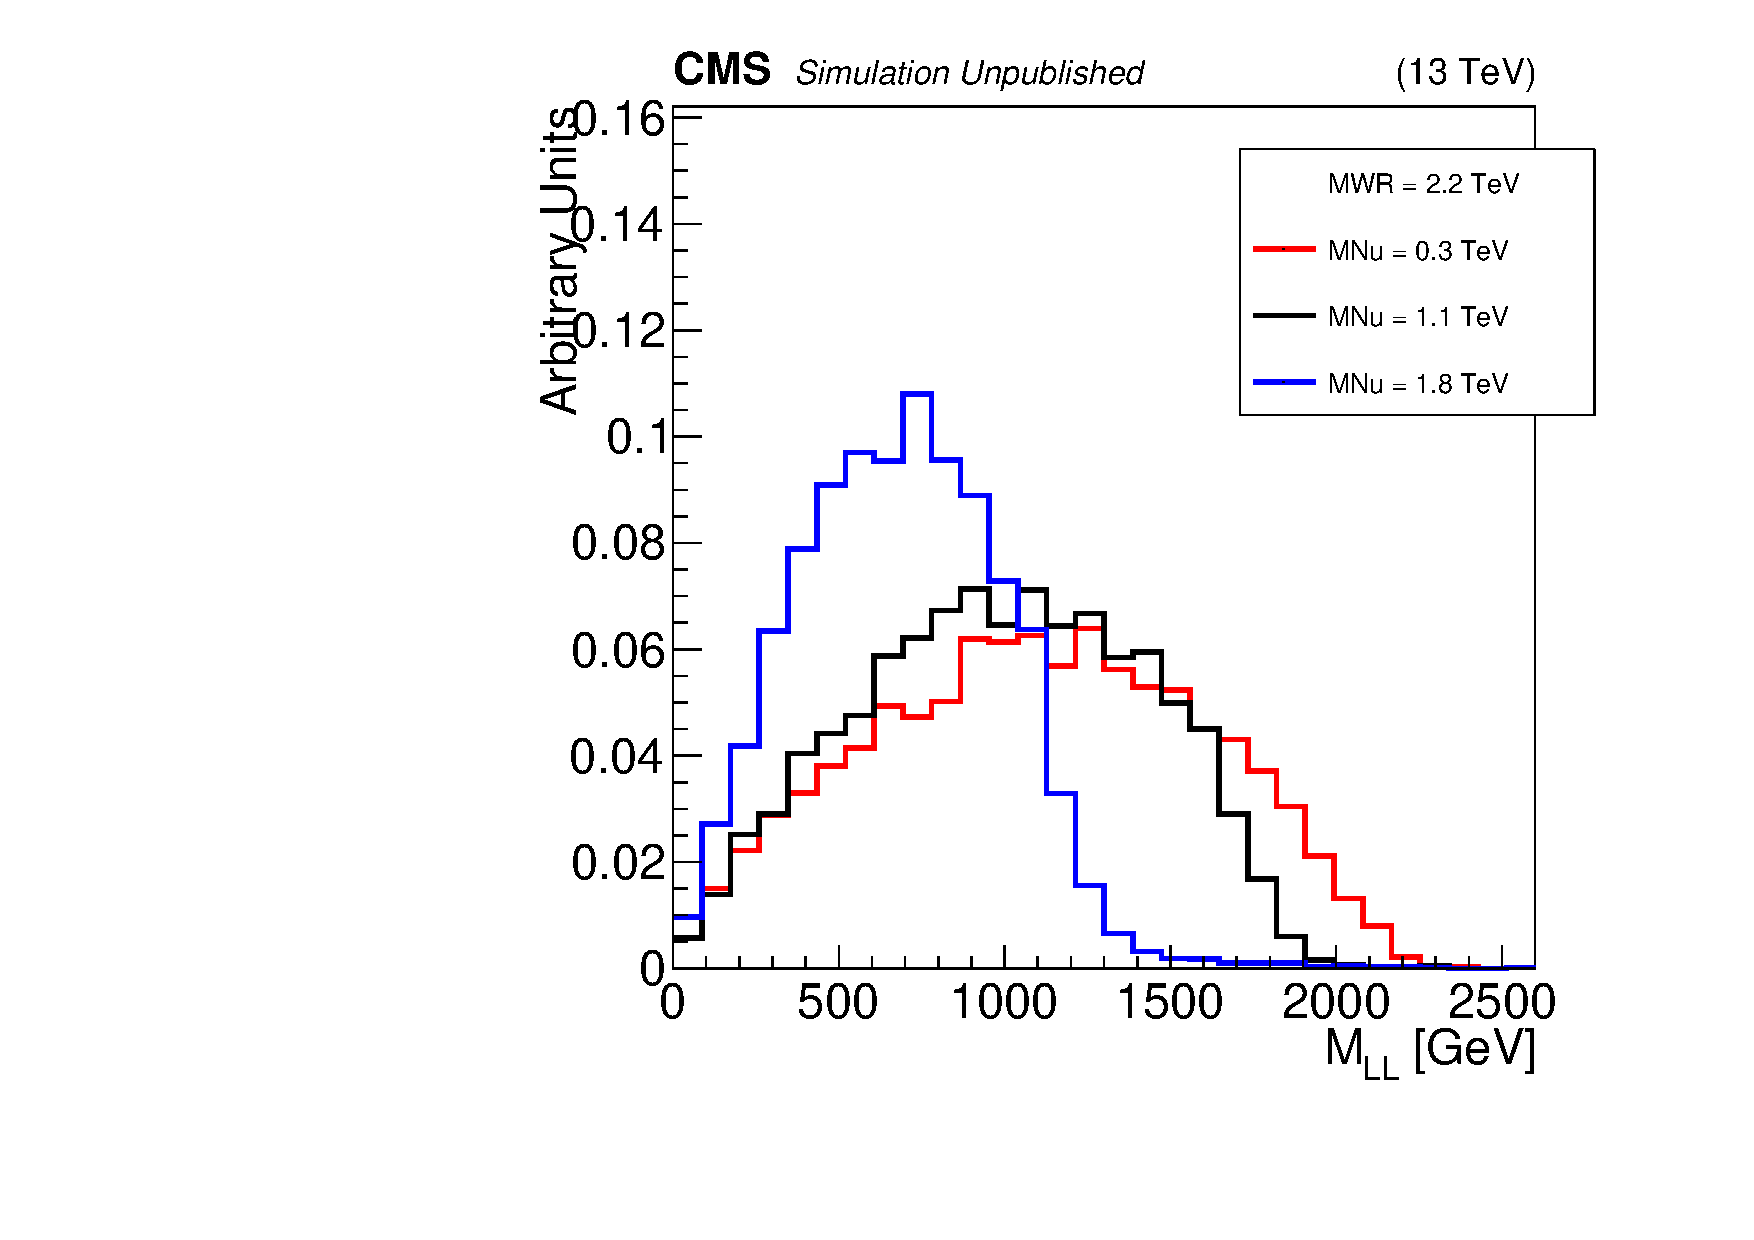
\includegraphics[width=0.5\textwidth]{figures/dileptonMassFromGenLeptonsFromFstAndScdHvyPtcl_MWR_2200_several_MNu_private.pdf}
	\caption{The $\Mll$ distribution of the two leptons produced in $\WR \rightarrow \ell\ell qq$ events with $\mWR = 2.2$ $\TeV$ and 
	different \mnul.}
	\label{fig:wrMllVarMNu}
\end{figure}

\clearpage

%\begin{figure}
%	\centering
%	\begin{subfigure}[t]{2.4in}
%		\centering
%		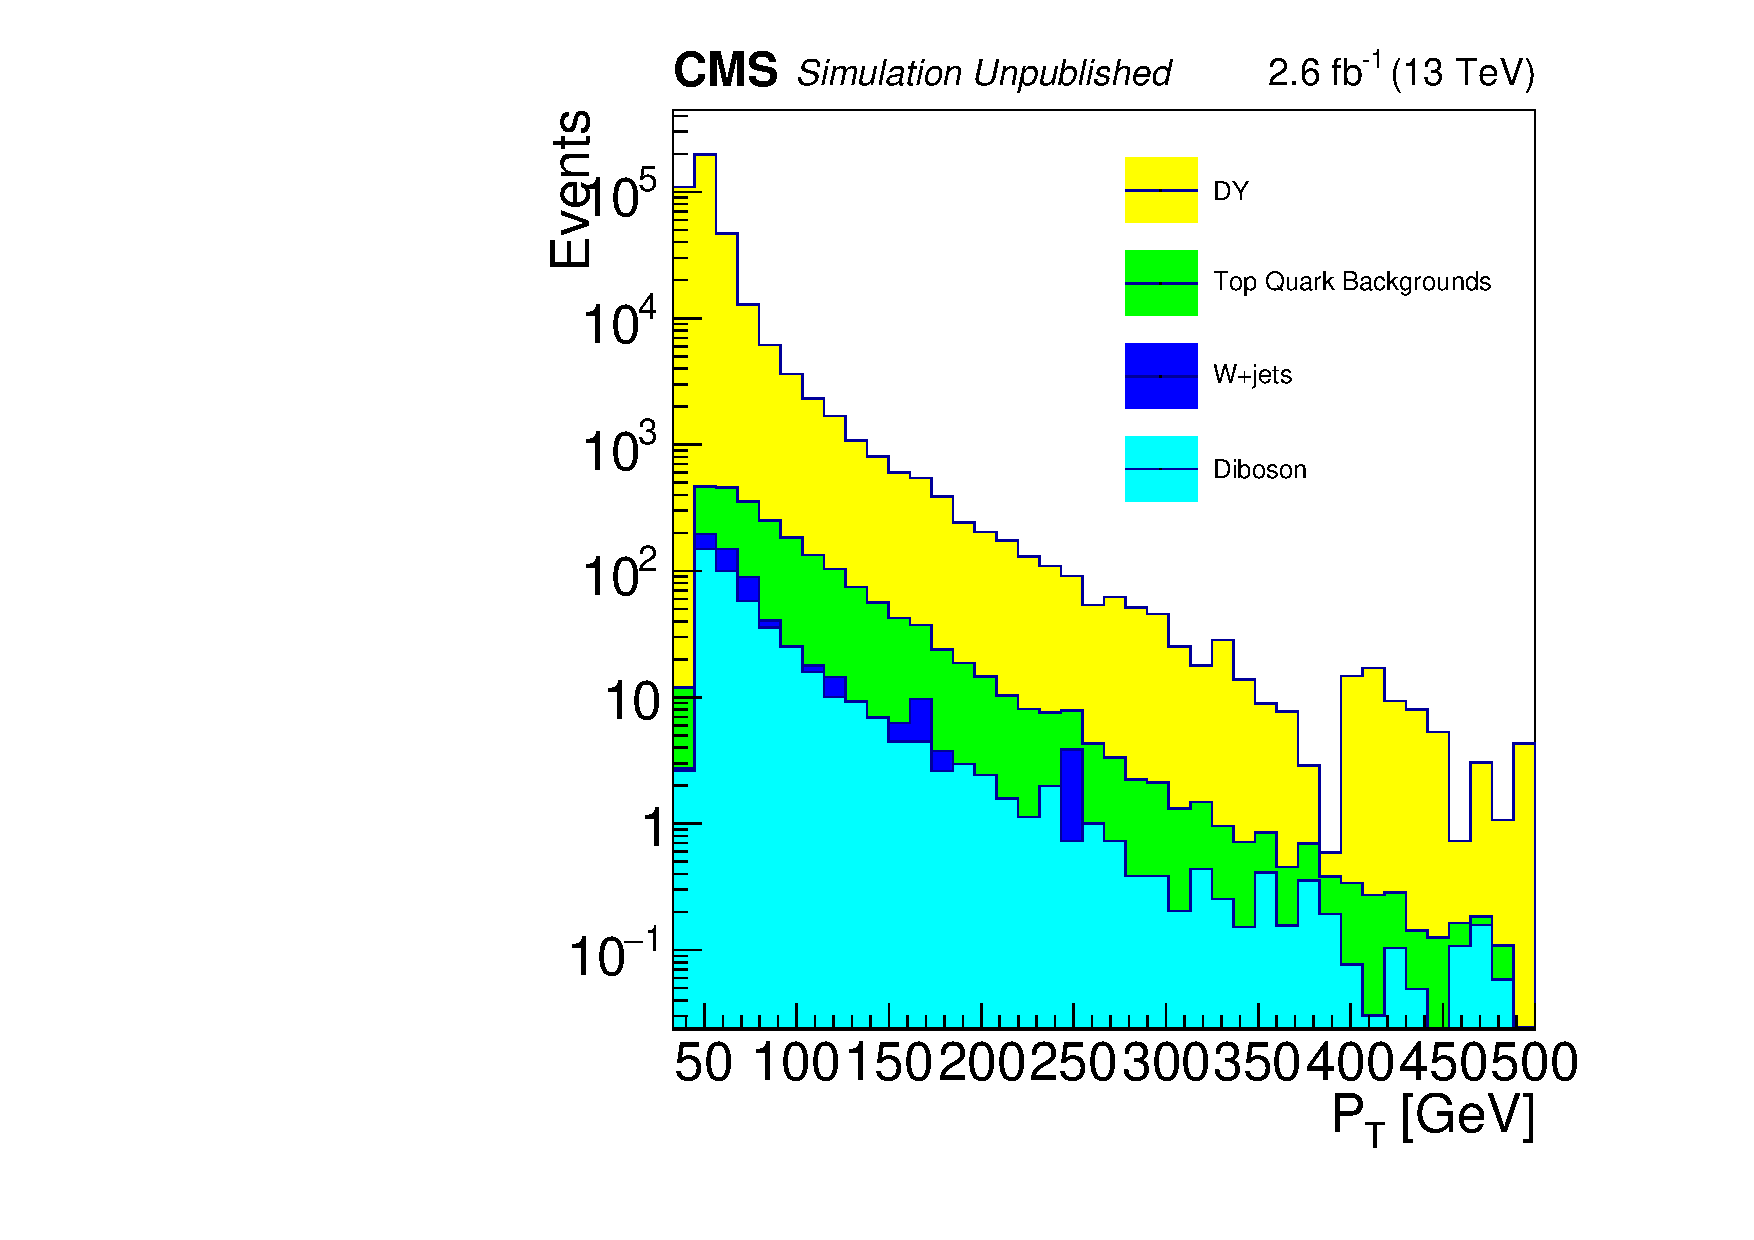
\includegraphics[width=2.4in]{figures/l1_pt_LooseSelection_TwoLeptsAndJets_EEChannelBkgndMC_log.pdf}
%		\caption{leading $\pt$ electron}\label{fig:bkgLeptJetPtsa}
%	\end{subfigure}
%	\thickspace
%	\begin{subfigure}[t]{2.4in}
%		\centering
%		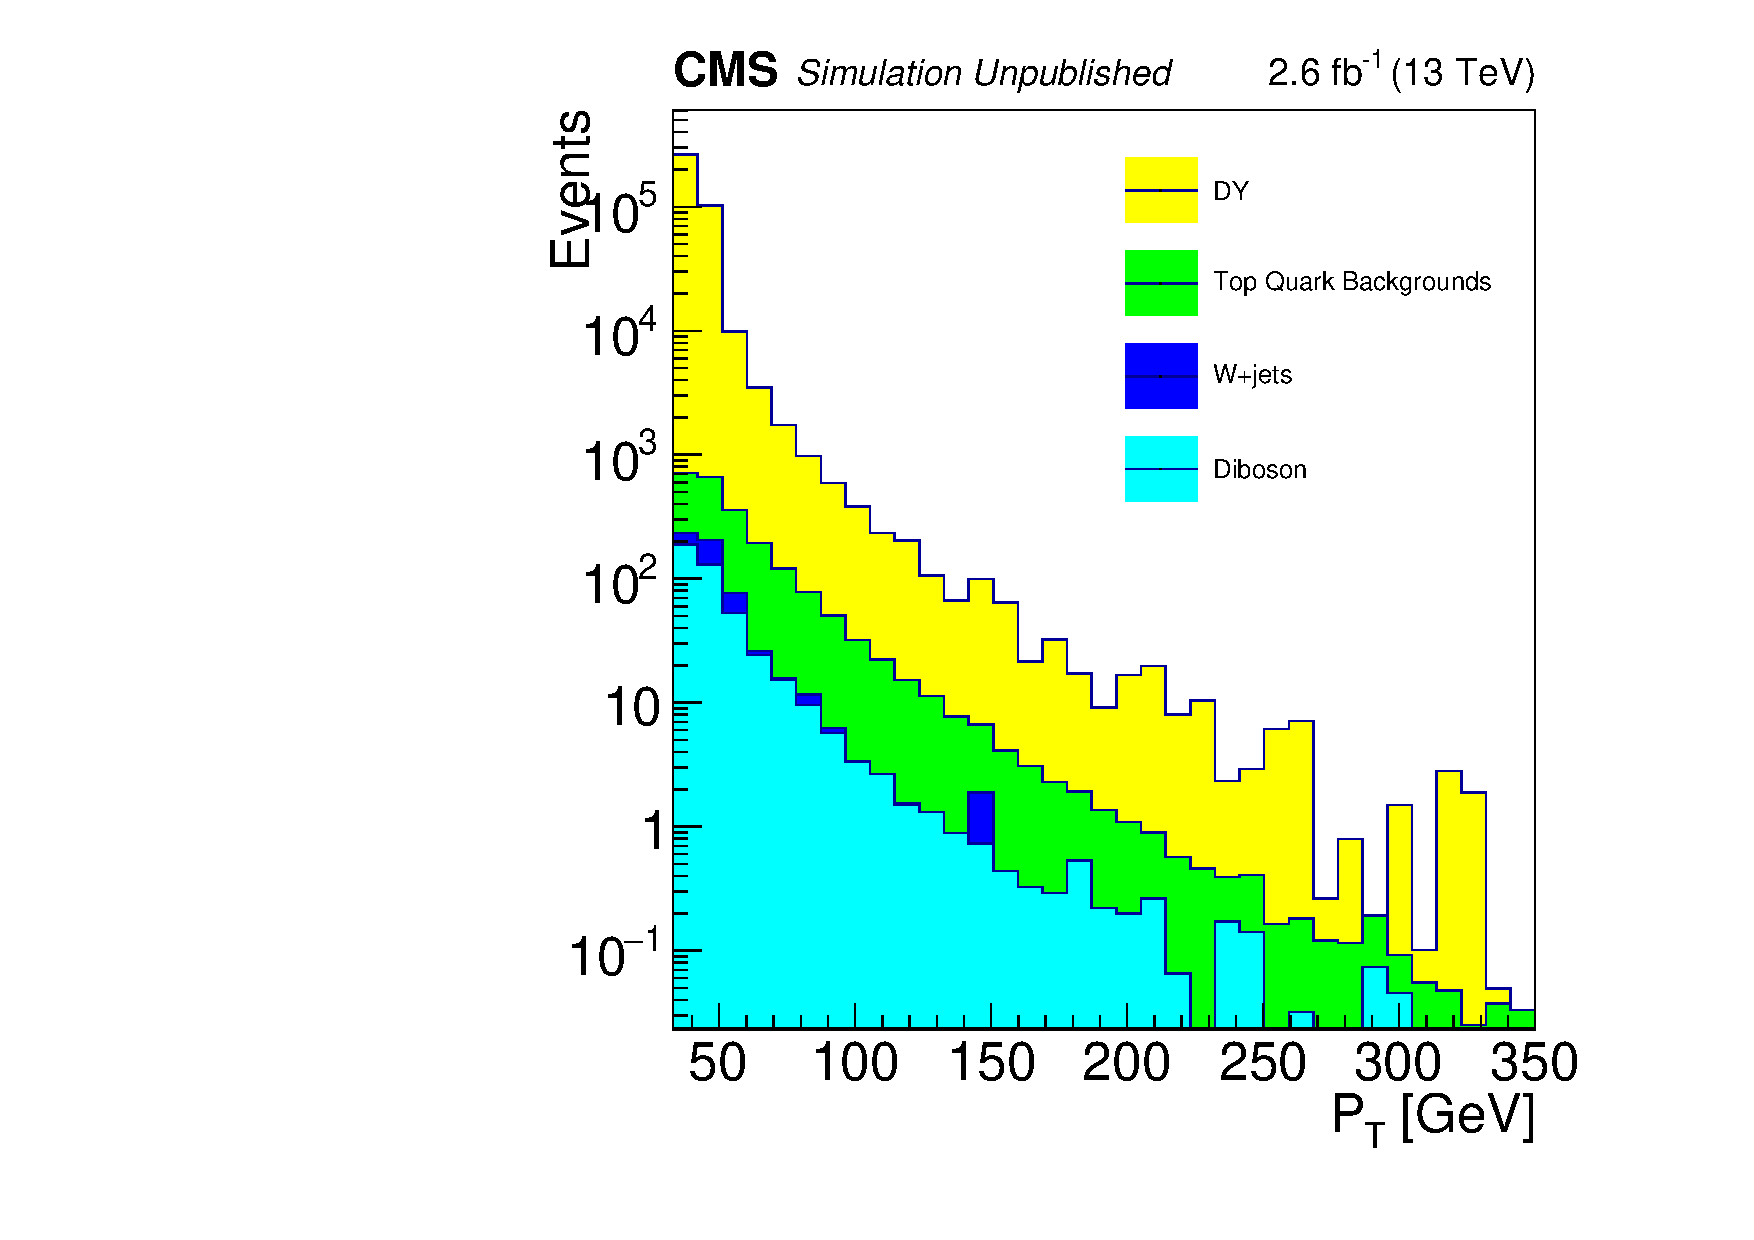
\includegraphics[width=2.4in]{figures/l2_pt_LooseSelection_TwoLeptsAndJets_EEChannelBkgndMC_log.pdf}
%		\caption{subleading $\pt$ electron}\label{fig:bkgLeptJetPtsb}
%	\end{subfigure}
%	\newline
%	\newline
%	\newline
%	\newline
%	\begin{subfigure}[t]{2.4in}
%		\centering
%		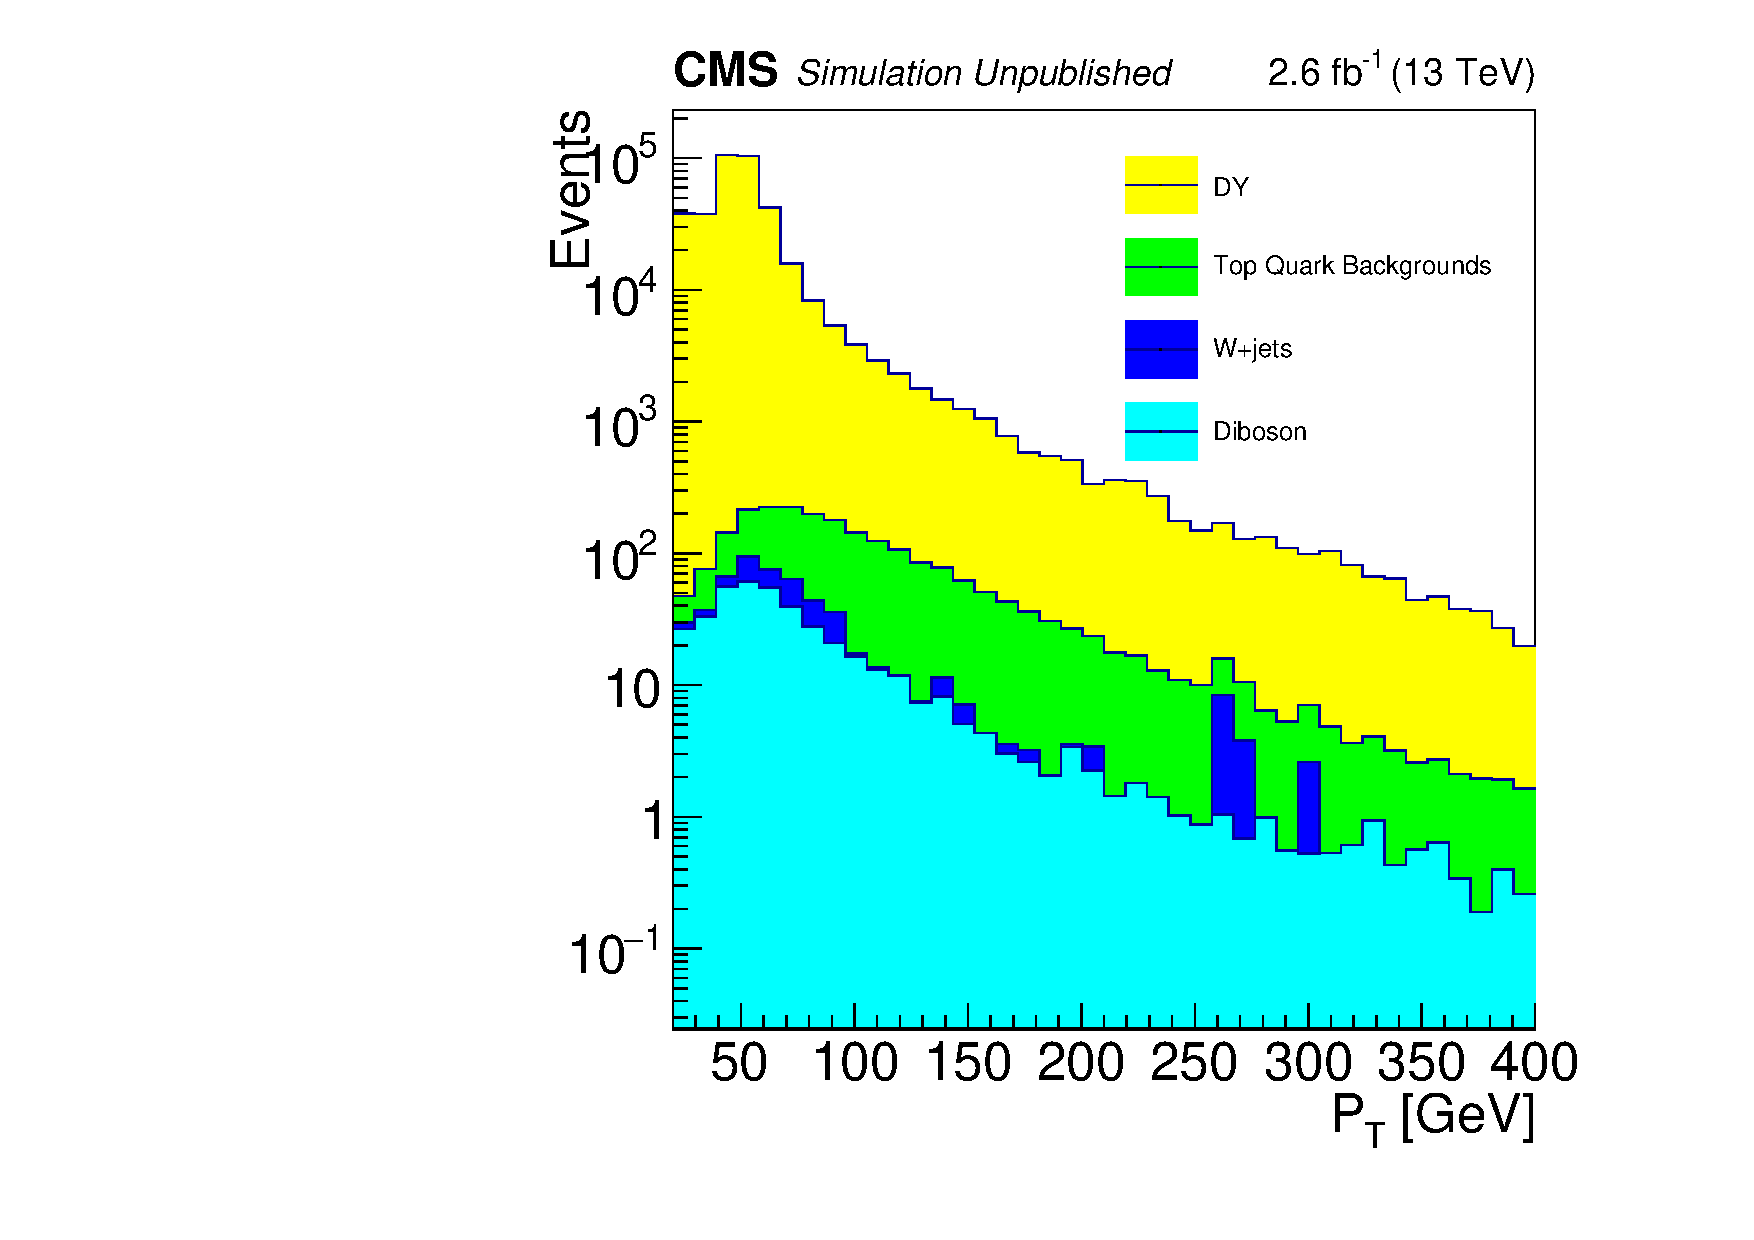
\includegraphics[width=2.4in]{figures/j1_pt_LooseSelection_TwoLeptsAndJets_EEChannelBkgndMC_log.pdf}
%		\caption{leading $\pt$ jet}\label{fig:bkgLeptJetPtsc}
%	\end{subfigure}
%	\thickspace
%	\begin{subfigure}[t]{2.4in}
%		\centering
%		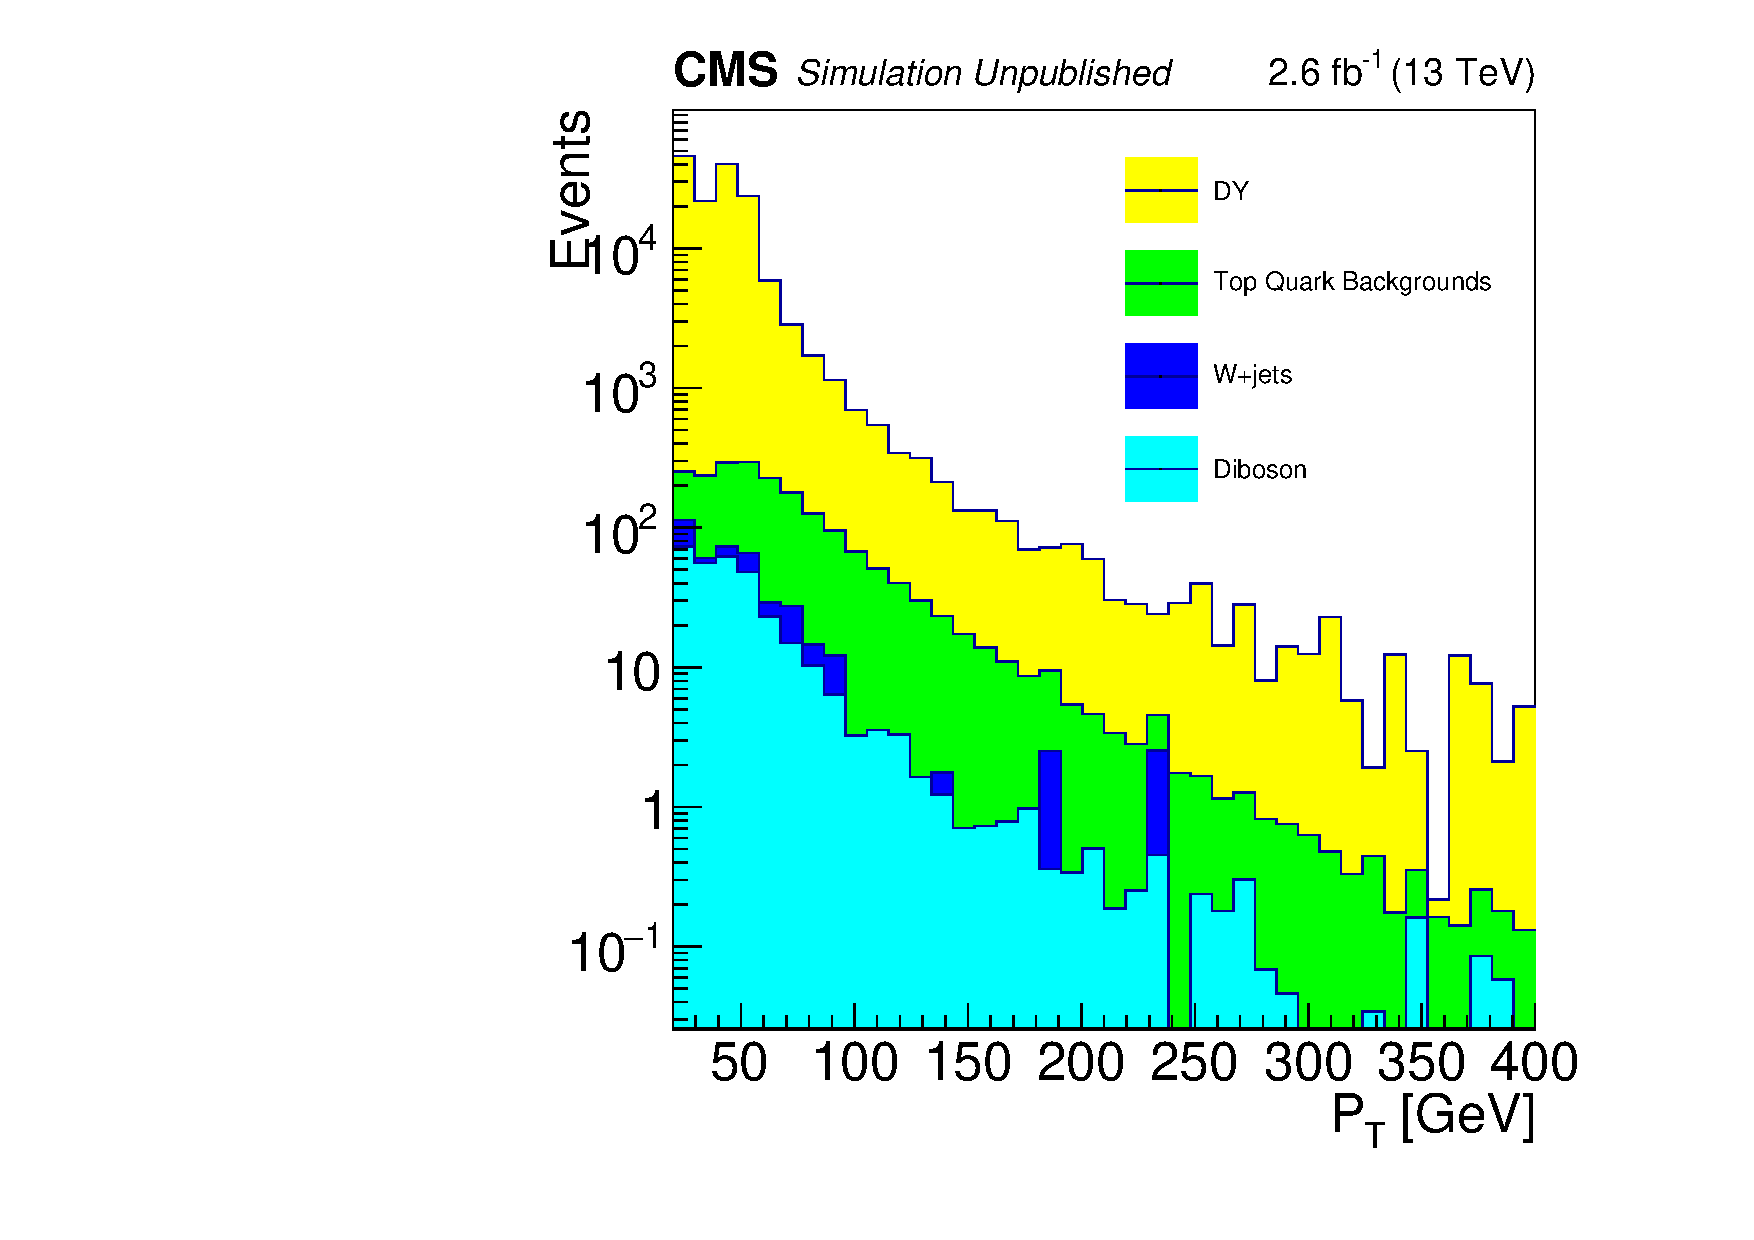
\includegraphics[width=2.4in]{figures/j2_pt_LooseSelection_TwoLeptsAndJets_EEChannelBkgndMC_log.pdf}
%		\caption{subleading $\pt$ jet}\label{fig:bkgLeptJetPtsd}
%	\end{subfigure}
%	\caption{The $\pt$ of electrons and jets reconstructed in simulated background events that passed the $ee$-channel offline ID and 
%	full online selection criteria.}\label{fig:bkgLeptJetPts}
%\end{figure}


\subsection{Offline Kinematic Selection Criteria}
\label{sec:offlineKinemSelCrit}
The kinematics of leptons and jets produced in \WR decays motivated the offline kinematic selection criteria.  These criteria are 
identical in the $ee$- and $\mu\mu$-channels.

The large expected \mWR and the reconstructed jet $\pt$ resolution motivated the jet $\pt$ and $\eta$ selection criteria.  The \WR decay 
produces two quarks in the central $|\eta|$ region (Figure \ref{fig:wrLeptJetEtas}), so each reconstructed event was required to have two 
jets in the region $|\eta| < 2.4$.  The $\pt$ of both jets scaled with the unknown ratio $\mnul/\mWR$, so the jet $\pt$ requirement was 
minimized to increase sensitivity to signals with low $\mnul/\mWR$.  The $\pt$ resolution of 
reconstructed jets that had $|\eta| < 1.3$ decreased rapidly below $\pt = 40$ $\GeV$: from 16\% or better resolution for $\pt > 40$ $\GeV$ to 
$\sim$21\% for $30 < \pt < 40$ $\GeV$ \cite{jetResolutionInCollisions}.  To avoid selecting low $\pt$ jets measured with poor $\pt$ 
resolution, the two jets in each event that had $|\eta| < 2.4$ were required to have $\pt > 40$ $\GeV$.  If more than two jets passed 
these criteria, the two highest $\pt$ jets were used.

The large expected \mWR and trigger selection criteria motivated the offline lepton $\pt$ and $\eta$ selection criteria.  For the same 
reason cited for the \WR quarks, the lepton progeny of the \WR are emitted in the central $|\eta|$ region (Figure \ref{fig:wrLeptJetEtas}) 
with high $\pt$ (Figure \ref{fig:wrLeptJetPts}).  Therefore, each event was required to have two leptons reconstructed with $|\eta| < 2.4$ 
and $\pt > 53$.  The 53 $\GeV$ threshold value was chosen so that leptons were selected in a $\pt$ range where the trigger efficiency was 
constant (Figure \ref{fig:trigEffs}).  In \WR decays one lepton is often produced with greater $\pt$ than the other, so at least one 
reconstructed lepton was required to have $\pt > 60$ $\GeV$.  This requirement increased sensitivity to a \WR signal relative to the ST 
backgrounds (Table \ref{tab:lowerLeptPtCut}).  If more than 2 leptons passed these criteria, the two highest $\pt$ leptons were used.

\begin{figure}
	\centering
	\begin{subfigure}[t]{2.4in}
		\centering
		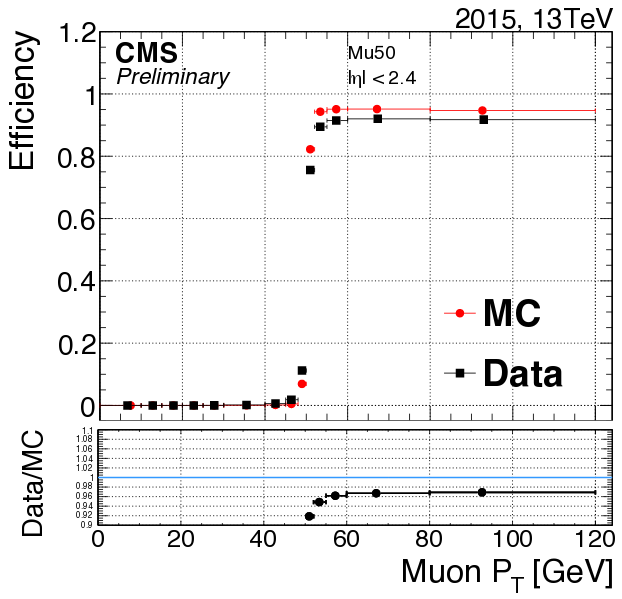
\includegraphics[width=2.4in]{figures/muonPt50TrgEffVsPt.png}
		%\caption{muon}\label{fig:trigEffsa}
	\end{subfigure}
	\newline
	\newline
	\newline
	\newline
	\begin{subfigure}[t]{2.4in}
		\centering
		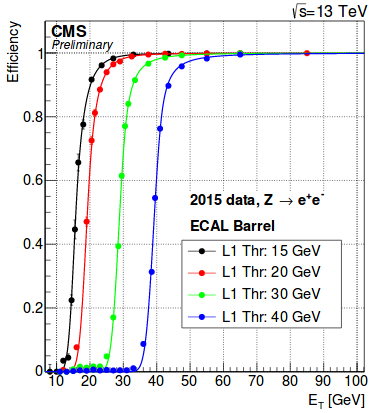
\includegraphics[width=2.4in]{figures/L1EGEfficiencyBarrel.png}
		%\caption{barrel electron}\label{fig:trigEffsb}
	\end{subfigure}
	\thickspace
	\begin{subfigure}[t]{2.4in}
		\centering
		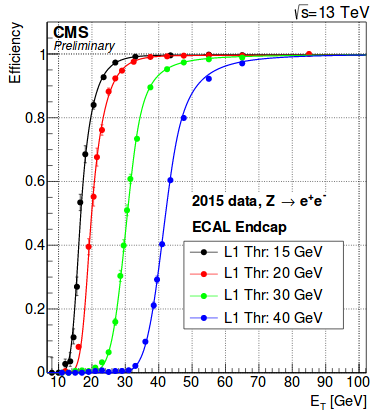
\includegraphics[width=2.4in]{figures/L1EGEfficiencyEndcap.png}
		%\caption{endcap electron}\label{fig:trigEffsc}
	\end{subfigure}
	\caption{The muon and electron trigger efficiencies versus $\pt$ or $\Et$ in $Z \rightarrow \ell\ell$ events.}\label{fig:trigEffs}
\end{figure}

\begin{table}[h]
	\caption{The signal (S) over background (B) sensitivity (S/$\sqrt{B}$) for different $\pt$ selection 
		criteria on the leading lepton.  The background is estimated using simulated \DY+jets and $t\bar{t}$ events, and the 
		signal is estimated using simulated $\WR \rightarrow \ell\ell jj$ events with $\mWR = 2.2 \TeV$ and $\mnul = 1.1 \TeV$.}
	\label{tab:lowerLeptPtCut}
	\centering
	\begin{tabular}{c|c}
		$\ell$ $\pt$ threshold ($\GeV$) & S/$\sqrt{B}$ \\  \hline
		53 &  11.7  \\
		60 &  12.6  \\ \hline
	\end{tabular}
\end{table}
\clearpage

Jets are clustered from reconstructed particles using the anti-$k_{T}$ algorithm with distance parameter $R = 0.4$.  If a particle is 
separated from a jet's axis by $\Delta R = G$, the distance parameter $R$ weights the likelihood of clustering that particle into the 
jet by $(\frac{0.4}{G})^{2}$.  The parameter $R$ constrains the maximum jet size, but it is possible for a reconstructed particle to be 
clustered into a jet and be separated from its axis by $\Delta R > 0.4$.  To avoid selecting a lepton reconstructed near a jet, each 
reconstructed lepton that passed the ID, $\pt$, and $\eta$ selection criteria was required to be separated from both selected jets by 
$\Delta R > 0.4$.

The \WR decay produces two high $\pt$ leptons whose dilepton mass $\Mll$, given by Equation \ref{eq:dileptMass}, increases as $\mnul/\mWR$ 
decreases and as \mWR increases.  Based on the high expected value of \mWR, the $\Mll$ selection requirement can safely exceed the $Z$ boson 
mass window of $60 < \Mll < 120$ $\GeV$ without adversely affecting the signal sensitivity.  However, the $\Mll$ requirement cannot be several 
hundred $\GeV$, otherwise the sensitivity to signal hypotheses with $\mnul/\mWR \sim$1 will decrease dramatically (Figure \ref{fig:wrMllVarMNu}).  
Knowing that the \DY and diboson backgrounds decrease rapidly with increasing $\Mll$, each event was required to have two leptons that had 
$\Mll > 200$ $\GeV$.  A lower threshold was not used because it would increase the background without a corresponding increase in the signal 
(Table \ref{tab:lowerMllCut}).

\begin{equation}
	\Mll = \sqrt{2|p_{1}||p_{2}|(1\thickspace - \thickspace \cos(\theta_{12}))}
	\label{eq:dileptMass}
\end{equation}

%\clearpage
%\begin{figure}[h]
%	\centering
%	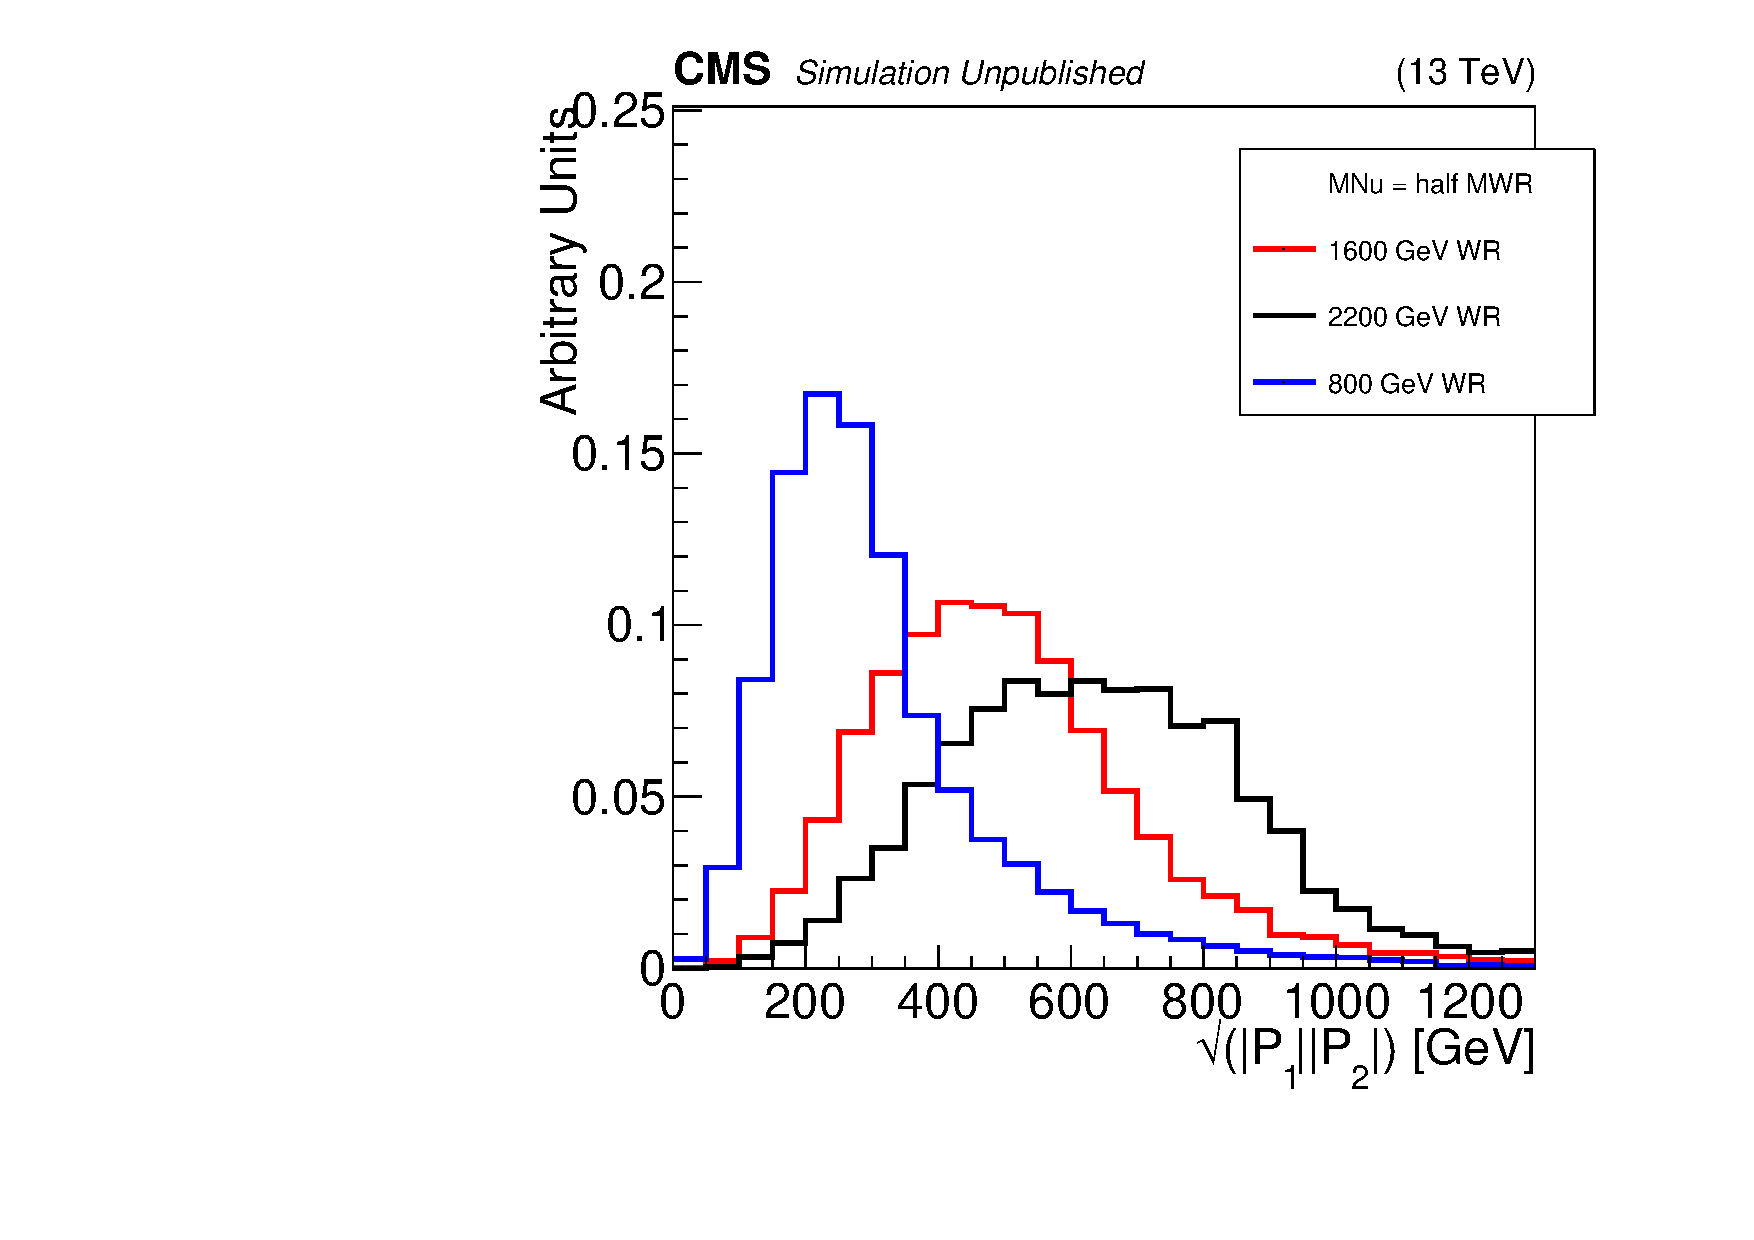
\includegraphics[width=0.5\textwidth]{figures/sqrtProdGenLeptMomentumMag_several_MWR_and_MNu_private.pdf}
%	\caption{The distribution of the square root of the product of the momentum magnitudes of the two leptons produced in $\WR \rightarrow \ell_{1}\ell_{2} qq$ 
%		events with several \mWR and $\mnul = \frac{1}{2}\mWR$.}
%	\label{fig:wrLeptSqrtMomMagVarMNu}
%\end{figure}

\begin{table}[h]
	\caption{The signal (S) over background (B) sensitivity (S/$\sqrt{B}$) for different $\Mll$ selection 
		criteria.  The background is estimated using simulated \DY+jets and $t\bar{t}$ events, and the 
		signal is estimated using simulated $\WR \rightarrow \ell\ell jj$ events with $\mWR = 2.2 \TeV$ and $\mnul = 1.1 \TeV$.}
	\label{tab:lowerMllCut}
	\centering
	\begin{tabular}{c|c}
		$\Mll$ threshold ($\GeV$) & S/$\sqrt{B}$ \\  \hline
		180 &  12.0  \\
		200 &  12.6  \\ \hline
	\end{tabular}
\end{table}
%\clearpage

Applying the previous selection criteria to simulated ST background events created a peak in the $\Mlljj$ distribution near 500 $\GeV$ 
(Figure \ref{fig:sculptedMlljj}).  To avoid this peak, each event was required to have $\Mlljj > 600$ $\GeV$.
\clearpage

\begin{figure}[h]
	\centering
	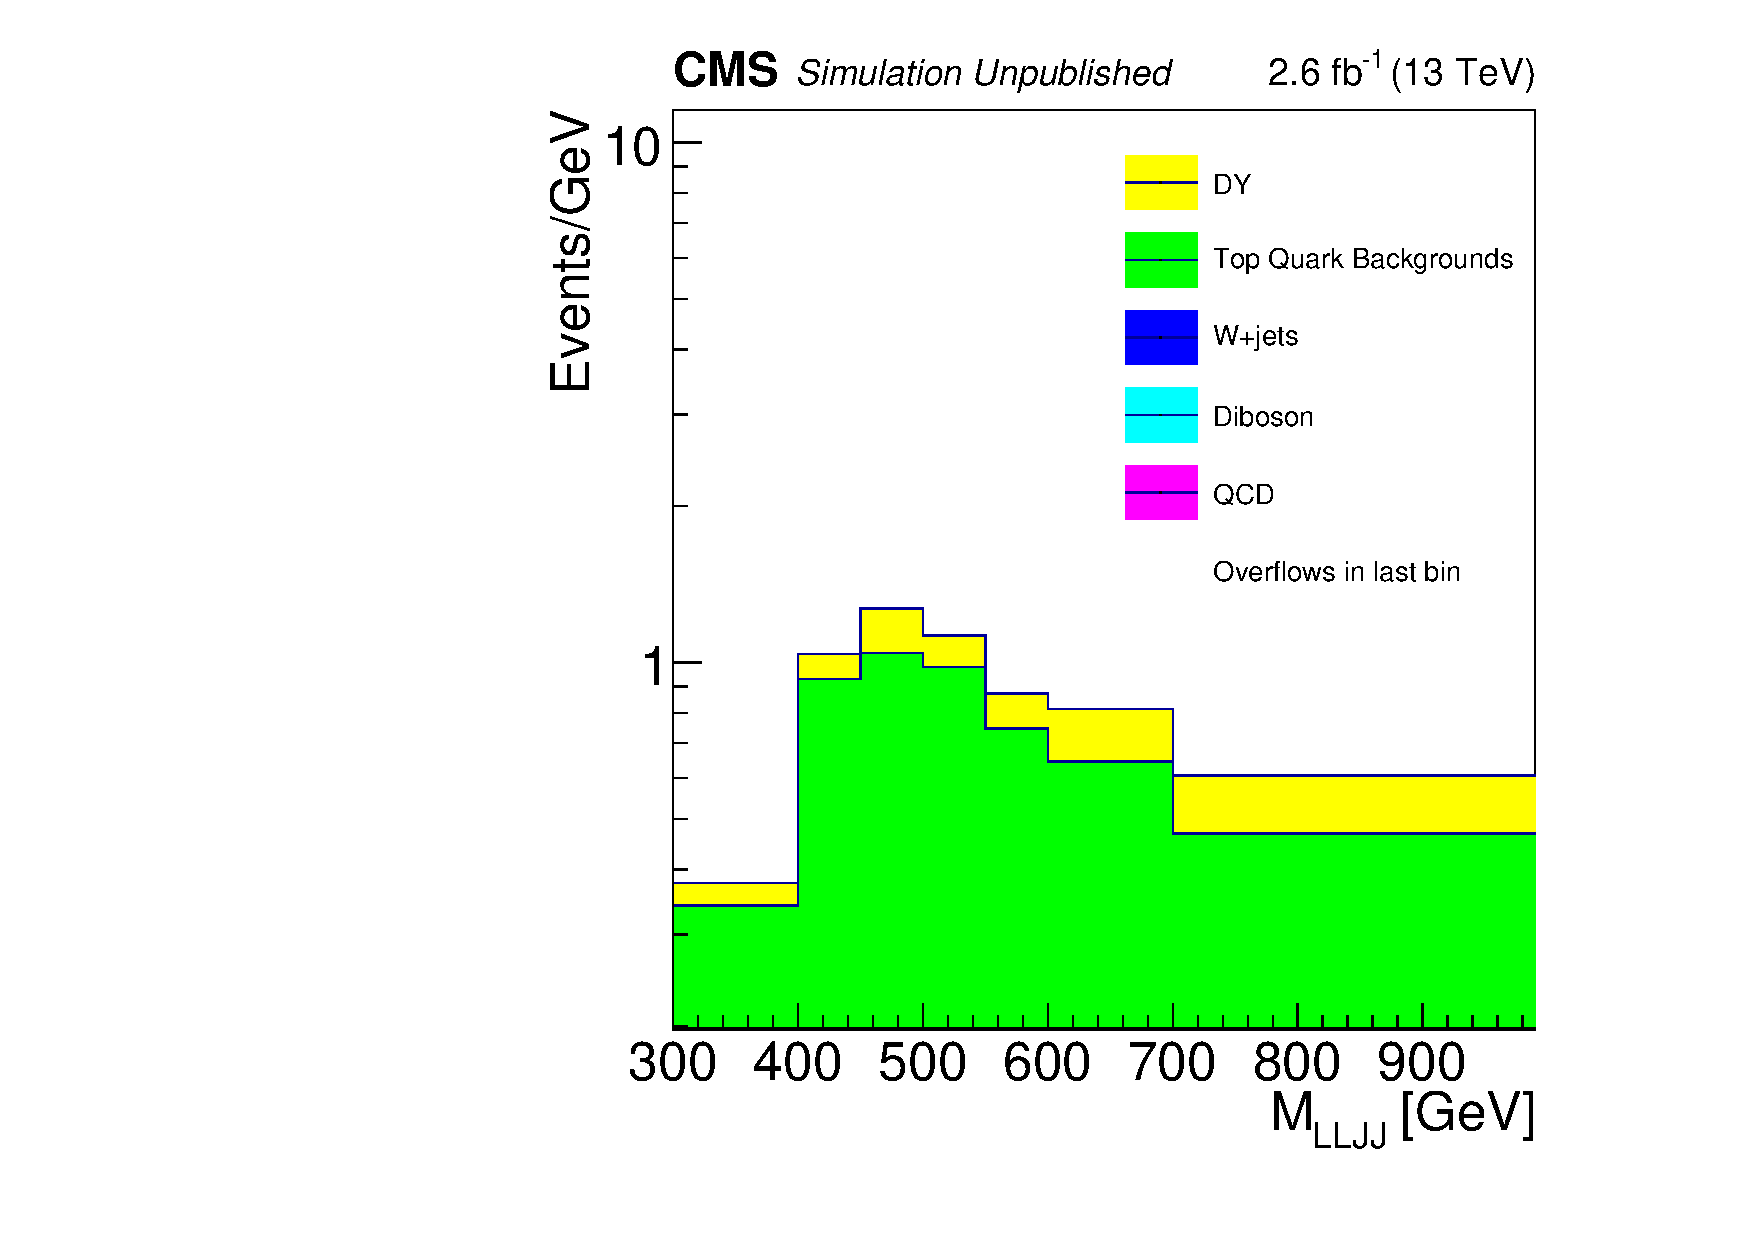
\includegraphics[width=0.45\textwidth]{figures/Mlljj_varBins_SignalRegion_EEChannelBkgndMC_DYMadHTAndIncl_TTBarFromData_log.pdf}
	\caption{The $\Mlljj$ distribution in simulated background events after applying the online criteria, and the offline ID and kinematic 
	selection criteria.}
	\label{fig:sculptedMlljj}
\end{figure}

The offline kinematic selection criteria (Table \ref{tab:offlineKinemSel}) were developed to select $\WR \rightarrow \ell\ell jj$ events 
over a large range of \mWR and \mnul values with the highest possible efficiency.  The selection efficiency of the full online and offline 
(ID and kinematic) selection criteria in signal events was estimated by simulating $pp \rightarrow \WR \rightarrow \ell\ell jj$ interactions, and 
applying the selection criteria to those events.  The \PYTHIA \MC generator implements a flexible, generic \WR signal model that captures the 
main characteristics of theoretical models discussed in the literature 
\cite{earlyLRSModel,lrsHiggsStageOne,lrsHiggsStageTwo,seeSawAndParityViolation,seeSawAndGUTs,lrsMassConstraints}, so \PYTHIA was used to 
simulate $\WR \rightarrow \ell\ell jj$ events with different \mWR and \mnul.  The trigger efficiency, offline ID and kinematic selection 
efficiency was calculated using 50000 event datasets produced with $\mnul = \frac{1}{2}\mwr$ and \mWR stepping from 0.8 to 6.0 $\TeV$ in 
increments of 0.2 $\TeV$.  At a given \mWR, only the offline kinematic selection efficiency varied by more than a few percent over the 
entire \mnul range.  The variation in the offline kinematic selection efficiency versus \mnul was calculated using 10000 event datasets 
produced with \mWR increasing from 0.8 to 4.0 $\TeV$ in increments of 0.1 $\TeV$.  Each 10000 event dataset was produced with a different \mnul 
that increased from 100 $\GeV$ to \mWR in increments of 0.1 $\TeV$ or less.  The total trigger, offline ID and kinematic selection efficiency (Figure 
\ref{fig:wrRecoSelectionEff}) exceeded 50\% in the $ee$-channel, and 70\% in the $\mu\mu$-channel.  The efficiency is lower in the $ee$-
channel due to the gap in ECAL coverage for $1.44 < |\eta| < 1.57$, and lower efficiency offline ID criteria applied to electrons 
relative to muons.  The variation in the offline kinematic selection efficiency versus \mnul (Figure \ref{fig:wrOffSelEffVarMWrMNu}) increases 
with \mWR: up to 30\% for $\mWR \leq 1.3$ $\TeV$, and up to 70\% for $\mWR \geq 2.5$ $\TeV$.  For a specific \mWR, the offline kinematic selection 
efficiency is maximized or nearly so when $\mnul = \frac{1}{2}\mWR$.

\begin{table}[h]
	\caption{The kinematic selection criteria applied to reconstructed leptons and jets that passed the offline identification 
	selection criteria.  The criteria were applied in the order that they are listed.}
	\label{tab:offlineKinemSel}
	\centering
	\begin{tabular}{c|c}
		parameter & threshold  \\  \hline
		lead jet $\pt,\eta$ & $\pt>40\GeV,|\eta|<2.4$ \\
		sublead jet $\pt,\eta$ & $\pt>40\GeV,|\eta|<2.4$ \\
		lead $\ell$ $\pt,\eta$ & $\pt>60\GeV,|\eta|<2.4$ \\
		sublead $\ell$ $\pt,\eta$ & $\pt>53\GeV,|\eta|<2.4$ \\
		$\Delta R(\ell,j)$ & $>0.4$ \\
		$\Mll$ & $>200\GeV$ \\
		$\Mlljj$ & $>600\GeV$ \\ \hline
	\end{tabular}
\end{table}

\begin{figure}[h]
	\centering
	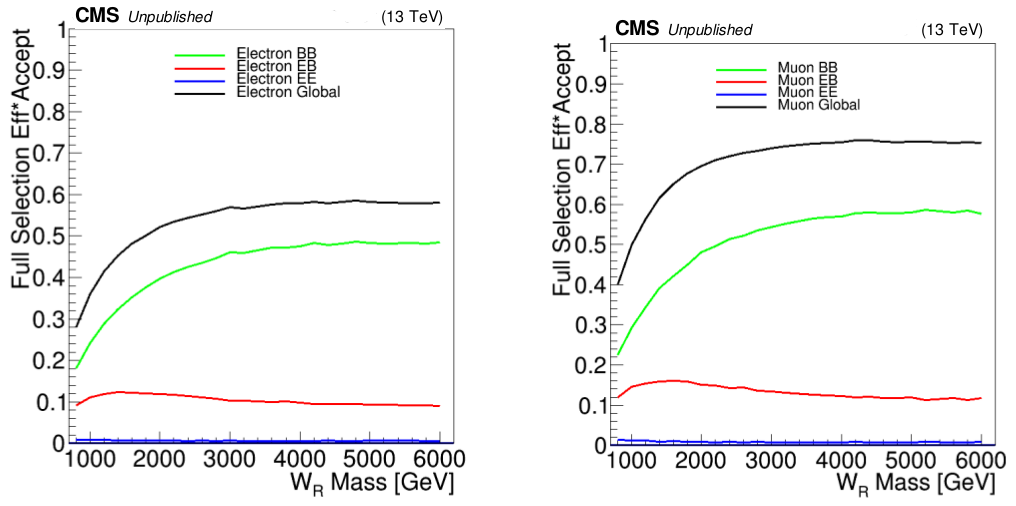
\includegraphics[width=1.0\textwidth]{figures/wrRecoSelectionEfficiency.png}
	\caption{The full selection efficiency in simulated $\WR \rightarrow \ell\ell jj$ events, in the $ee$-channel (left) and the 
		$\mu\mu$-channel (right).  Different curves represent events where both leptons are in the barrel (BB), one was in the 
	endcap (EB), or both were in the endcap (EE).}
	\label{fig:wrRecoSelectionEff}
\end{figure}
\clearpage


\begin{figure}[h]
	\centering
	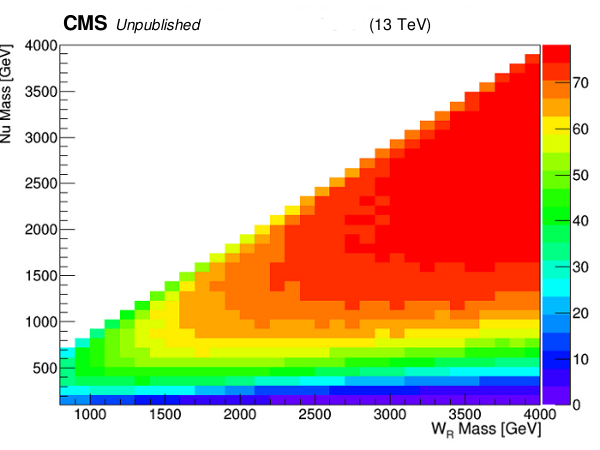
\includegraphics[width=1.0\textwidth]{figures/genWrMuMuAccEff_NoMassWindows13TeV.png}
	\caption{The offline kinematic selection efficiency (\%) in $\WR \rightarrow \ell\ell jj$ events versus \mWR and \mnul.}
	\label{fig:wrOffSelEffVarMWrMNu}
\end{figure}

\clearpage

\section{Reconstruction and Selection Summary}
\label{sec:recoConclusion}
Electrons, muons and jets expected from \WR and \nul decays are reconstructed from signals measured in CMS sub-detectors using dedicated 
reconstruction algorithms.  These algorithms reconstruct leptons, hadrons and jets with high efficiency by using minimal selection criteria, 
and occasionally ($\sim$1-3\%) reconstruct individual particles and jets incorrectly.  The contribution of incorrectly 
reconstructed particles to $\ell\ell jj$ events was reduced by requiring leptons and jets to pass identification (ID) selection criteria.  
Selected particles were then required to pass kinematic selection criteria to identify particles whose kinematics are consistent with \WR 
decay kinematics.  After applying all selection criteria to data events, the selected events were used to make a $\Mlljj$ distribution.  
The decay $\WR \rightarrow \ell\ell jj$ transfers all energy of the \WR into the invariant mass of the leptons and jets, so evidence of a 
\WR, independent of \mnul, was searched for as an excess of data events above predicted backgrounds in the $\Mlljj$ distribution.  The 
$\Mlljj$ distribution found in data due to backgrounds was predicted using data and simulated events in $\ell\ell jj$ control regions with 
no signal contamination.  The selection criteria of the control regions and the resulting background predictions are discussed in the next 
chapter.


%%%%%%%%%%%%%%%%%%%%%%%%%%%%%%%%%%%%%%%%%%%%%%%%%%%%%%%%%%%%%%%%%%%%%%%%%%%%%%%%
